%!TEX root = ../thesis.tex
%*******************************************************************************
%****************************** Fifth Chapter *********************************
%*******************************************************************************

\chapter{A comparative analysis to distinguish β-cell states and investigate shared transcriptional signatures across T2D-related stressors
}
\label{chapter3}
\newpage

\begin{Comment2}
\vspace{3mm}
\label{contr:chapter2}
\hspace{-3mm}
\textbf{Statement of Contributions} \\\\

\end{Comment2}

\clearpage

% \section{\( \mathbf{\upbeta} \)-cell heterogeneity and adaptation in response to stress}

% In any given multicellular biological system, cellular heterogeneity  can arise from developmental programs establishing cellular subtypes, from changes in cellular state due to altered environments or cell-intrinsic fluctuations, and from stochastic variation in gene expression. Cellular heterogeneity has been shown to be involved in development, adaptation to dynamic environmental conditions, repair and regeneration, as well as disease.
% While it has long been apparent that not all β-cells in adult islets are identical, recent technological advances have shed further light on β-cell heterogeneity in terms of their morphology, identity and function. Although GSIS is the key function of mature β-cells, some β-cells may also retain non-secretory roles, necessary for overall islet function \textbf{\cite{liu_all_2017}}. This heterogeneity in β-cells is driven by topography and developmental origin \textbf{\cite{puri_plasticity_2015,roscioni_impact_2016}}, maturation state \textbf{\cite{salinno_-cell_2019}}, and stress response \textbf{\cite{xin_pseudotime_2018}}. Recent advances in characterization of β-cell heterogeneity have raised several important questions about the physiological significance of the prevalence of different β-cell sub-populations, , their role in diabetes pathogenesis, and the plasticity of individual β-cells.

% \subsection{Previously established \( \mathbf{\upbeta} \)-cell heterogeneity}
% \colorbox{pink}{missing figure} \colorbox{green}{text clean-up} \colorbox{orange}{incomplete text} \\
% \subsubsection{Historical Perspective}
% In a study from 1960, Hellerström \textit{et. al.} identified regional differences in nuclear sizes and the position of nucleoli within the nuclei, depending on whether the β-cells were located centrally or peripherally in large or small islets in rat. The authors further suggested that these cytological differences could be interpreted as corresponding differences in functional states of β-cells, as lower activity in centrally located β-cells in large islets could be due to cells being older or due to lower concentrations of glucose and/or insulin, compared to the cells in the periphery or in small islets \textbf{\cite{hellerstrom_properties_1960}}. In 1986, Salomon and Meda demonstrated that β-cells in rat islets were heterogeneous in their ability to release insulin \textbf{\cite{salomon_heterogeneity_1986}}. In particular, the group of Daniel G. Pipeleers carried out pioneering work in characterizing and describing β-cell heterogeneity in rodents; they identified distinct β-cell sub-populations differing in glucose responsiveness, insulin secretion and NADPH levels \textbf{\cite{kiekens_differences_1992,schuit_glucose_1988,van_de_winkel_autofluorescence-activated_1983}}.

% \subsubsection{\( \mathbf{\upbeta} \)-cell diversity: Insights from single-cell RNA sequencing (scRNA-seq)}
% The field of single-cell biology has revolutionized the characterization of cells and led to the identification of novel cell-types, cell states and a better understanding of mechanisms in health and diseases. This topic has been discussed in detail in \textbf{\hyperref[sec:scrna]{Section 1.5}}. Single-cell analyses have recapitulated the previously described idea concept of functional β-cell heterogeneity and \hl{....}  Another study identified that mature and immature and/or proliferative β-cells co-exist in healthy mouse islets. The immature β-cell cluster was characterized by downregulation of genes involved in insulin secretion, oxidative phosphorylation (OxPhos) and cell-cycle inhibition, as well as upregulation of genes involved in \textit{cAMP} and \textit{WNT} signaling. Further, trajectory inference %(see \hyperref[sec:sc_tpi]{TI methods}) 
% suggested a continuum of transition between the immature and mature states, rather than discrete phenotypes \textbf{\cite{sachs_targeted_2020}}. In another study employing mouse models, the authors defined β-cell maturity using arbitrarily defined levels of \textit{Pdx1} and \textit{Mafa}, and showed that adult islets are composed of mature (\textit{Pdx1}\textsuperscript{\textit{high}} \textit{Mafa}\textsuperscript{\textit{high}}) and immature (\textit{Pdx1}\textsuperscript{\textit{low}} \textit{Mafa}\textsuperscript{\textit{low}}) β-cells and the balanced proportion of these sub-populations might contribute to proper islet function and insulin release \textbf{\cite{nasteska_pdx1low_2021}}. Another study demonstrated the adaptive plasticity of β-cells to reversible chronic ER stress wherein β-cells undergo a reprogramming of their transcriptome and proteome. More than half of the genes involved in ER protein processing as well as markers of β-cell identity were compromised due to chronic stress whereas upon alleviation, β-cells regained their mature identity. The authors postulated that the heterogeneity in the maturity of β-cells in the islets might be a physiological response to cycles of ER stress and recovery in vivo \textbf{\cite{chen_adaptation_2022}}.\\\\
% With recent advances in the throughput of single-cell experiments, accumulating single-cell data and multiple scRNA-seq data analysis and integration approaches, large reference atlases, which comprise of millions of cells across several tissues, organs, developmental stages and/or conditions are now routinely generated \textbf{\cite{regev_human_nodate}}. These atlases help understand cellular heterogeneity, and provide an opportunity to learn from several single-cell datasets simultaneously, allowing for automatic annotation of new datasets and easy comparative analyses across several conditions \textbf{\cite{rood_impact_,lotfollahi_mapping_2021}}. The integrated \gls{mia} by Hrovatin \textit{et. al.} \textbf{\cite{hrovatin_delineating_2023}}, represents a comprehensive scRNA-seq atlas of mouse pancreatic islets, integrating over 300,000 cells across multiple developmental stages and disease conditions. The study also provided insights into the heterogeneity and dynamic states of β-cells during development, aging, and under diabetic conditions and revealed an intermediate β-cell state between healthy controls and the different diabetes models, depicted heterogeneous expression of known β-cell maturity and dysfunction markers across β-cell states and described pathways indicative of the different  β-cell dysfunction phenotypes. Overall, the \gls{mia} complemented the growing body of research on islet β-cell biology and highlighted the critical role of high-resolution single-cell atlases. 

% \subsection{\( \mathbf{\upbeta} \)-cell adaptation and response to stress}
% \colorbox{pink}{missing figure} \colorbox{yellow}{missing text} \\

% The pathogenesis of \gls{t2d} is intricately linked to the dynamic response of β-cells to insulin resistance, wherein increased insulin demand is met by compensatory increases of insulin release, in order to maintain blood glucose homeostasis. It is evident from rodent studies that, both, expansion of β-cell mass and enhanced β-cell function are important for β-cell compensation. 


% The failure of β-cells to compensate for insulin resistance results in overt diabetes. β-cell dysfunction is characterized by loss of identity and lack of function.\\\\
% A central component of β-cell dysfunction in \gls{t2d} is the loss of functional mature identity and return to a progenitor-like state, termed as `dedifferentiation'. The dedifferentiation process is attributed to several factors such as oxidative stress, gluco- and lipo-toxicity, pro-inflammatory cytokines and altered gene expression.\\
% In particular, using PAGA, Hrovatin et. al further deciphered the relationship between healthy and diseased states by identifying a shared intermediate state prior to the T1D or T2D model state. Further examination of this intermediate state revealed differences in expression of most of the shared diabetes DEGs between healthy and intermediate states and further changed in the diabetic states. Based on these observations, the authors concluded that the intermediate state could represent a snapshot of the progression of β-cell dysfunction during diabetes. 


% %Based on clinical observations and work with animal models of diabetes, Weir \& Bonner-Weir proposed five stages of β-cell dysfunction during diabetes progression \textbf{\cite{weir_five_2004}}. The stages describe changes in β-cell mass, phenotype and function, ranging from initial compensation (Stage-1) with increased insulin secretion and intact β-cell function, through adaptation (Stage-2) and early decompensation (Stage-3) characterized by rising glucose levels and β-cell de-differentiation, to stable (Stage-4) and severe (Stage-5) decompensation marked by significant loss of β-cell mass and function. 


% % Failure of β-cell compensation is the defining event during the progression of \gls{t2d}. 

\clearpage

\section{An integrated atlas of pancreatic islet \( \mathbf{\upbeta} \)-cells across\\various models of \( \mathbf{\upbeta} \)-cell adaptation and decompensation}
\label{sec:int_atlas}
To better understand the mechanisms underlying successful and failed β-cell compensatory responses, we integrated seven scRNA-seq datasets. We included five datasets generated in-house that included broad ranges of increases in β-cell workload (\textbf{Fig. \ref{fig:3-1} A, Supplementary Table \ref{tab3-1}}), defined as insulin demand per β-cell. We further incorporated two previously published datasets to include  additional hyperglycemic models: islets from older \textit{ob/ob} animals, termed \textbf{Severe genetic obesity} \textbf{\cite{chung_endocrine-exocrine_2020}} and islets from mice subjected to 



\vspace{0.5cm}

\begin{figure}[H]
\centering
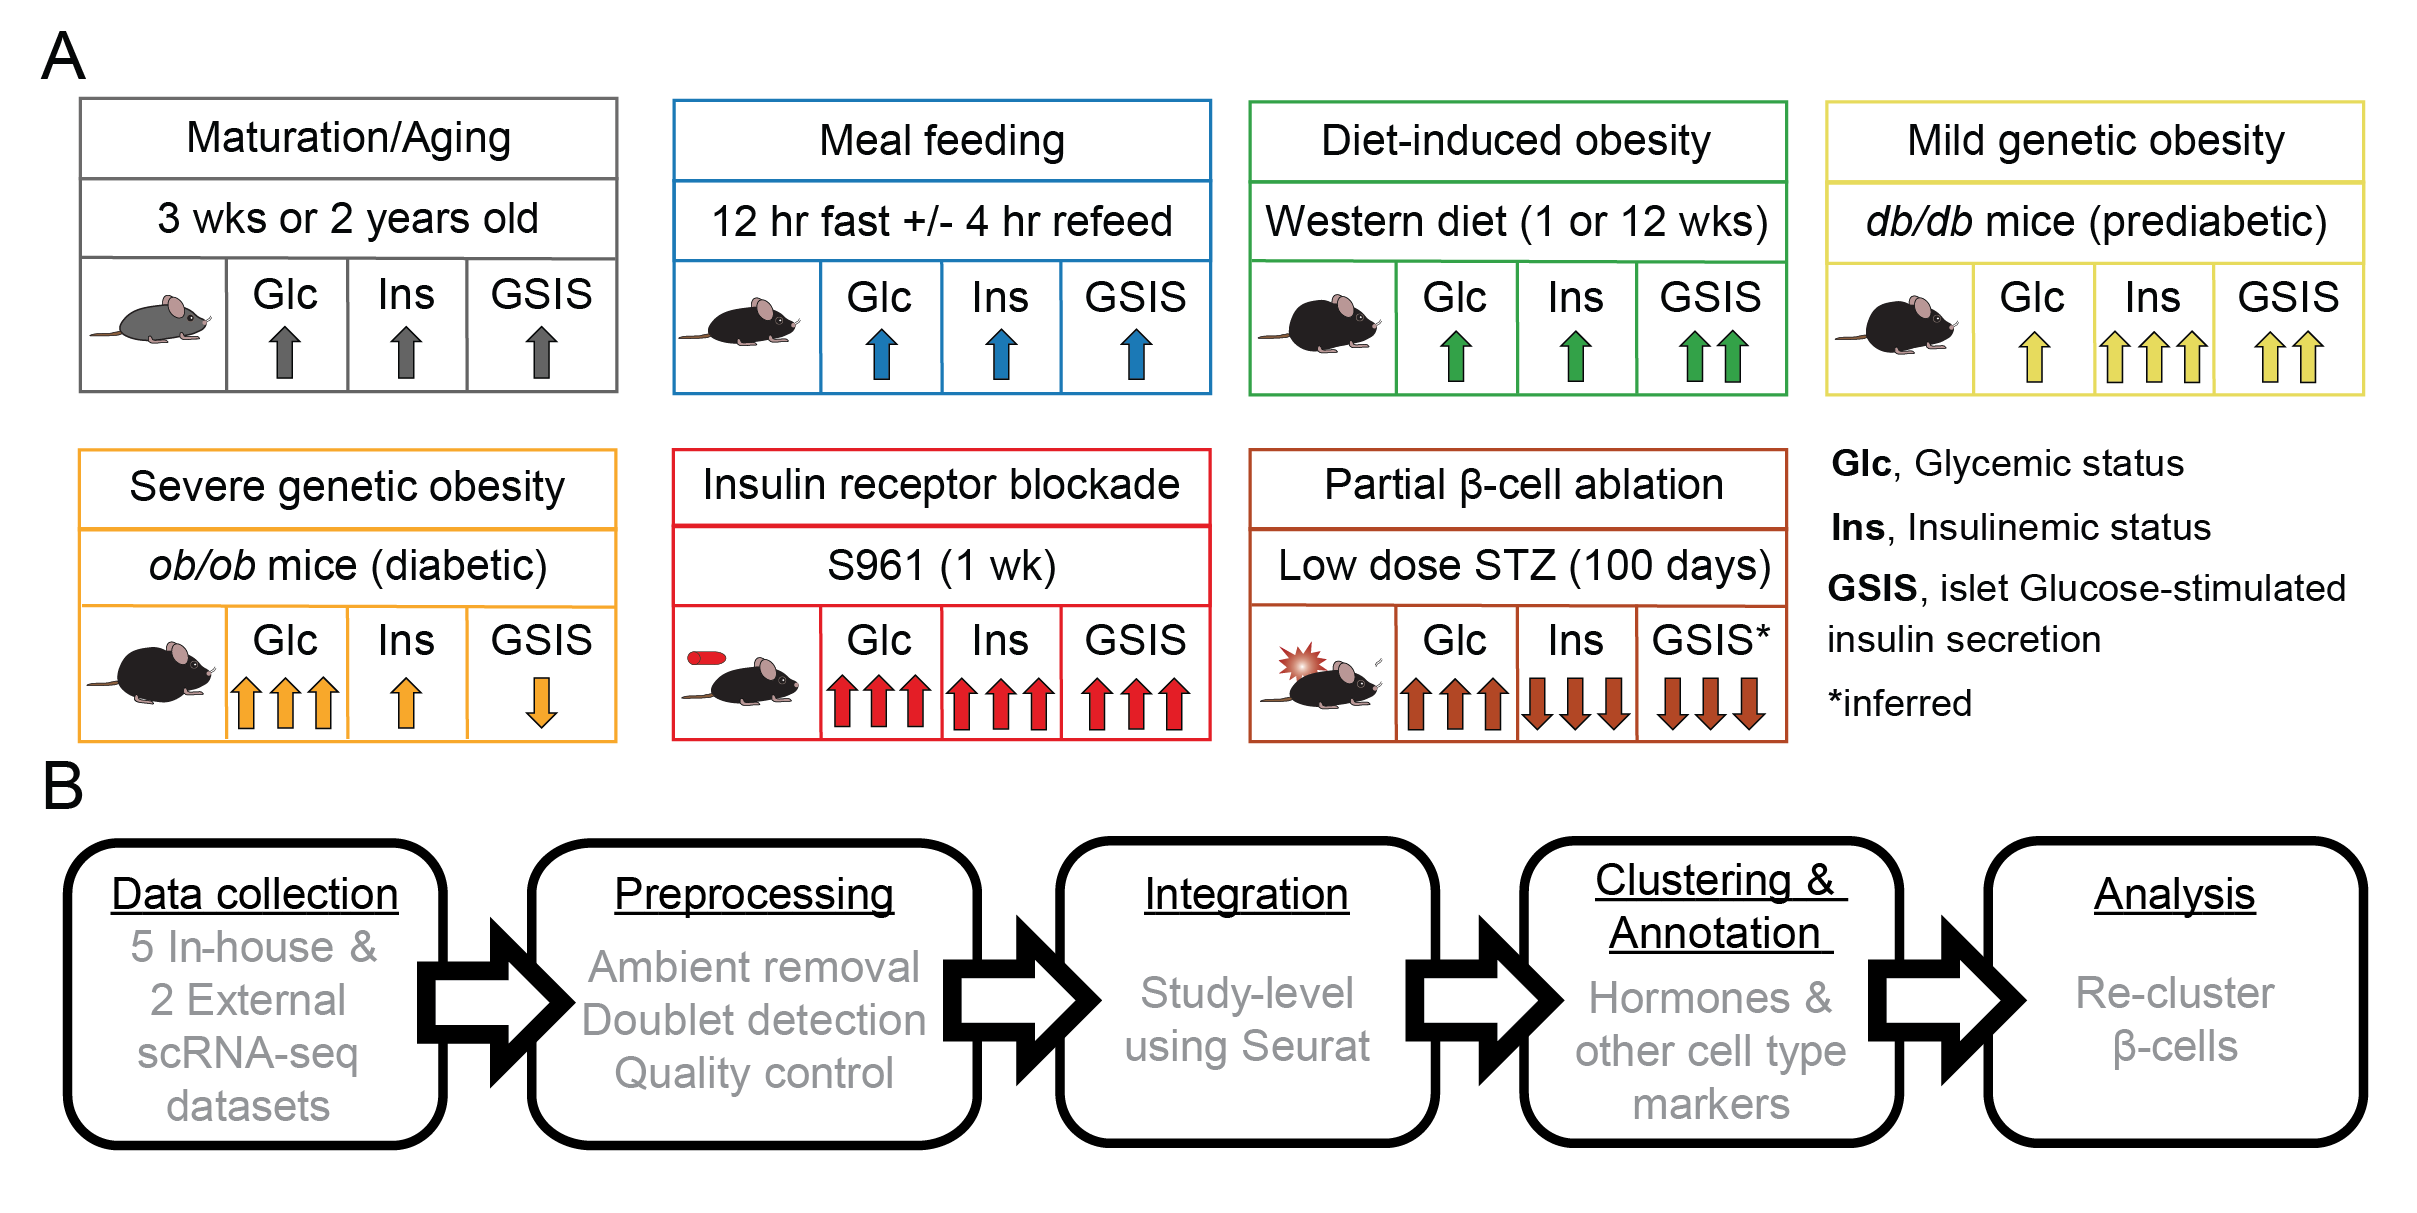
\includegraphics[width=\linewidth]{Chapter5/Fig/F3-1-v2-02.png}
\caption[Workflow to build an integrated atlas to study β-cell transcriptome]{\textbf{Integrated atlas to study β-cell transcriptome in various states that increase workload.} \textbf{(A)} Overview of the various β-cell workload models used in this study. For every model, the effect of the workload on the glycemic, insulinemic and GSIS status of the animals is indicated. The orientation of the arrows indicate the directionality of the response while the number of arrows indicate the intensity. \textbf{(B)} A schematic depicting the workflow for preprocessing, integration, clustering and further downstream analysis.}
\label{fig:3-1}
\end{figure}

%\clearpage

partial β-cell ablation by \gls{stz}, termed \textbf{Partial β-cell ablation} \textbf{(Fig. \ref{fig:3-1} A)} \textbf{\cite{sachs_targeted_2020}}. The samples across the seven datasets varied primarily across age (Supplementary Table \ref{tab3-1}). An additional study incorporating islets from 3-week-old (3 wks) or 2-year-old mice, termed \textbf{Maturation/aging}, was used as a reference point for developmental maturity. The same study, along with the data from \textbf{Diet-induced obesity} model were also utilized for the comprehensive analysis of islet-associated immune cells in (\textbf{Chapter \ref{chapter2}}). Out of the seven studies, six of them isolated islets exclusively from male mice, whereas the \textbf{Meal feeding} dataset pooled islets from both male and female mice (Supplementary Table \ref{tab3-1}). Integration of the datasets to be included in the atlas allowed us to account for the various batch-effects arising from sample handling, housing conditions, and mouse strains used. We applied the same pre-processing steps with individual thresholds for every sample across the seven datasets. To enable joint analysis and comparisons of the datasets, we performed data integration in order to create a joint embedding space (\textbf{Fig. \ref{fig:3-1} B}, see \textit{Methods}).\\

% \begin{figure}[H]
% \centering
% 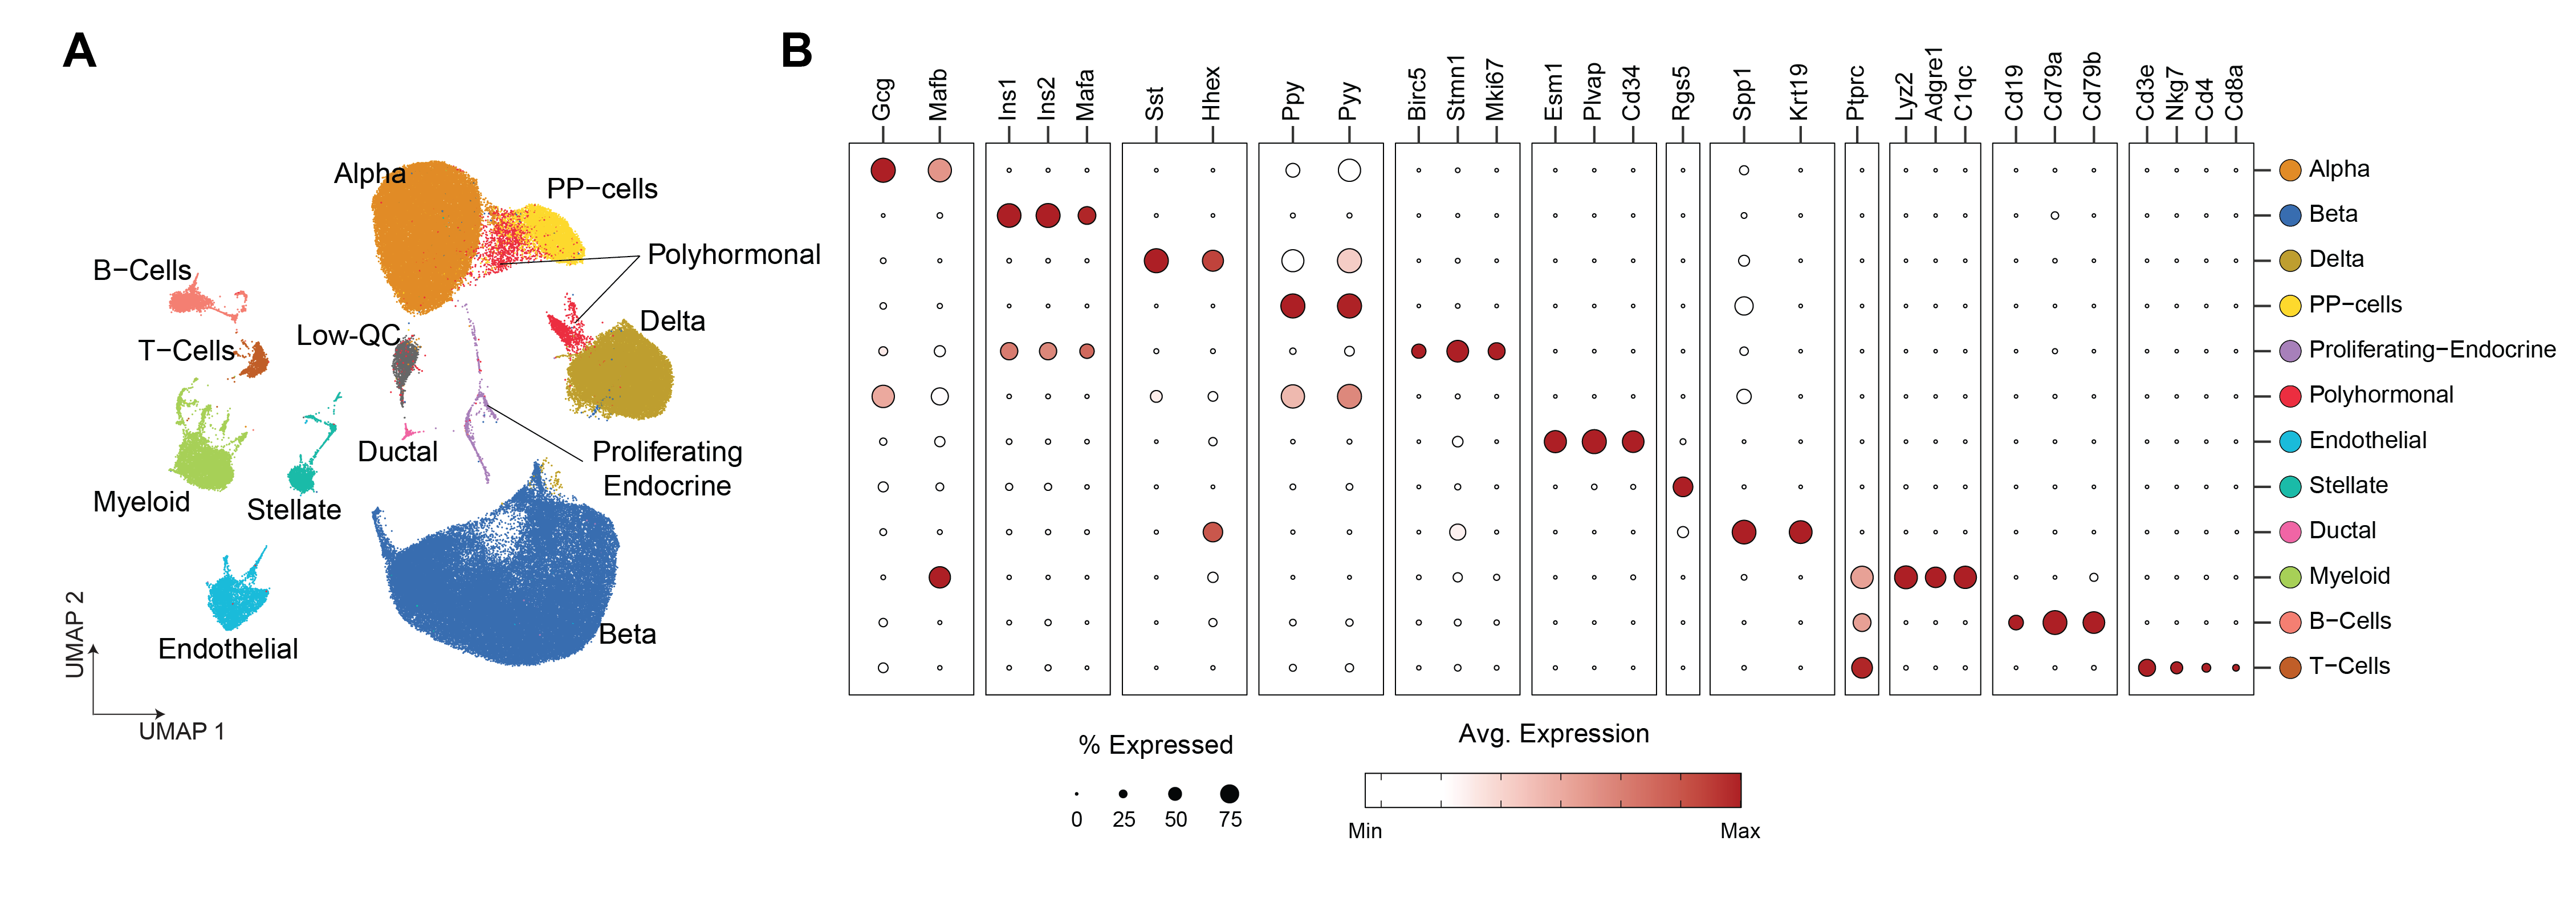
\includegraphics[width=\linewidth]{Chapter5/Fig/F3-2-01.png}
% \caption[fig3-2]{\textbf{Integrated dataset of seven scRNA-seq studies across several models of β-cell decompensation and hyperglycemia.}\\
% \textbf{(A)} UMAP embedding of the integrated dataset depicting celltype annotations based on the expression of known markers. \textbf{(B)} UMAP embedding of the integrated dataset depicting the seven scRNA-seq studies. Datasets are described in Supplementary Table \ref{tab3-1}. \textbf{(C)} Number of cells per sample within each study. \textbf{(D)} Dotplot depicting hallmark markers for the annotated celltypes in panel \textbf{A}. \textbf{E} Number of cells per celltype.}
% \label{fig:3-2}
% \end{figure}
% \clearpage


% \captionof{figure}{\textbf{Integrated dataset of seven scRNA-seq studies across several models of β-cell decompensation and hyperglycemia.} \textbf{(A)} UMAP embedding of the integrated dataset depicting celltype annotations based on the expression of known markers. \textbf{(B)} UMAP embedding of the integrated dataset depicting the seven scRNA-seq studies. Datasets are described in Supplementary Table \ref{tab3-1}. \textbf{(C)} Number of cells per sample within each study. \textbf{(D)} Dotplot depicting hallmark markers for the annotated celltypes in panel \textbf{A}. \textbf{E} Number of cells per celltype.}

%\clearpage

\begin{figure}[H]
\centering
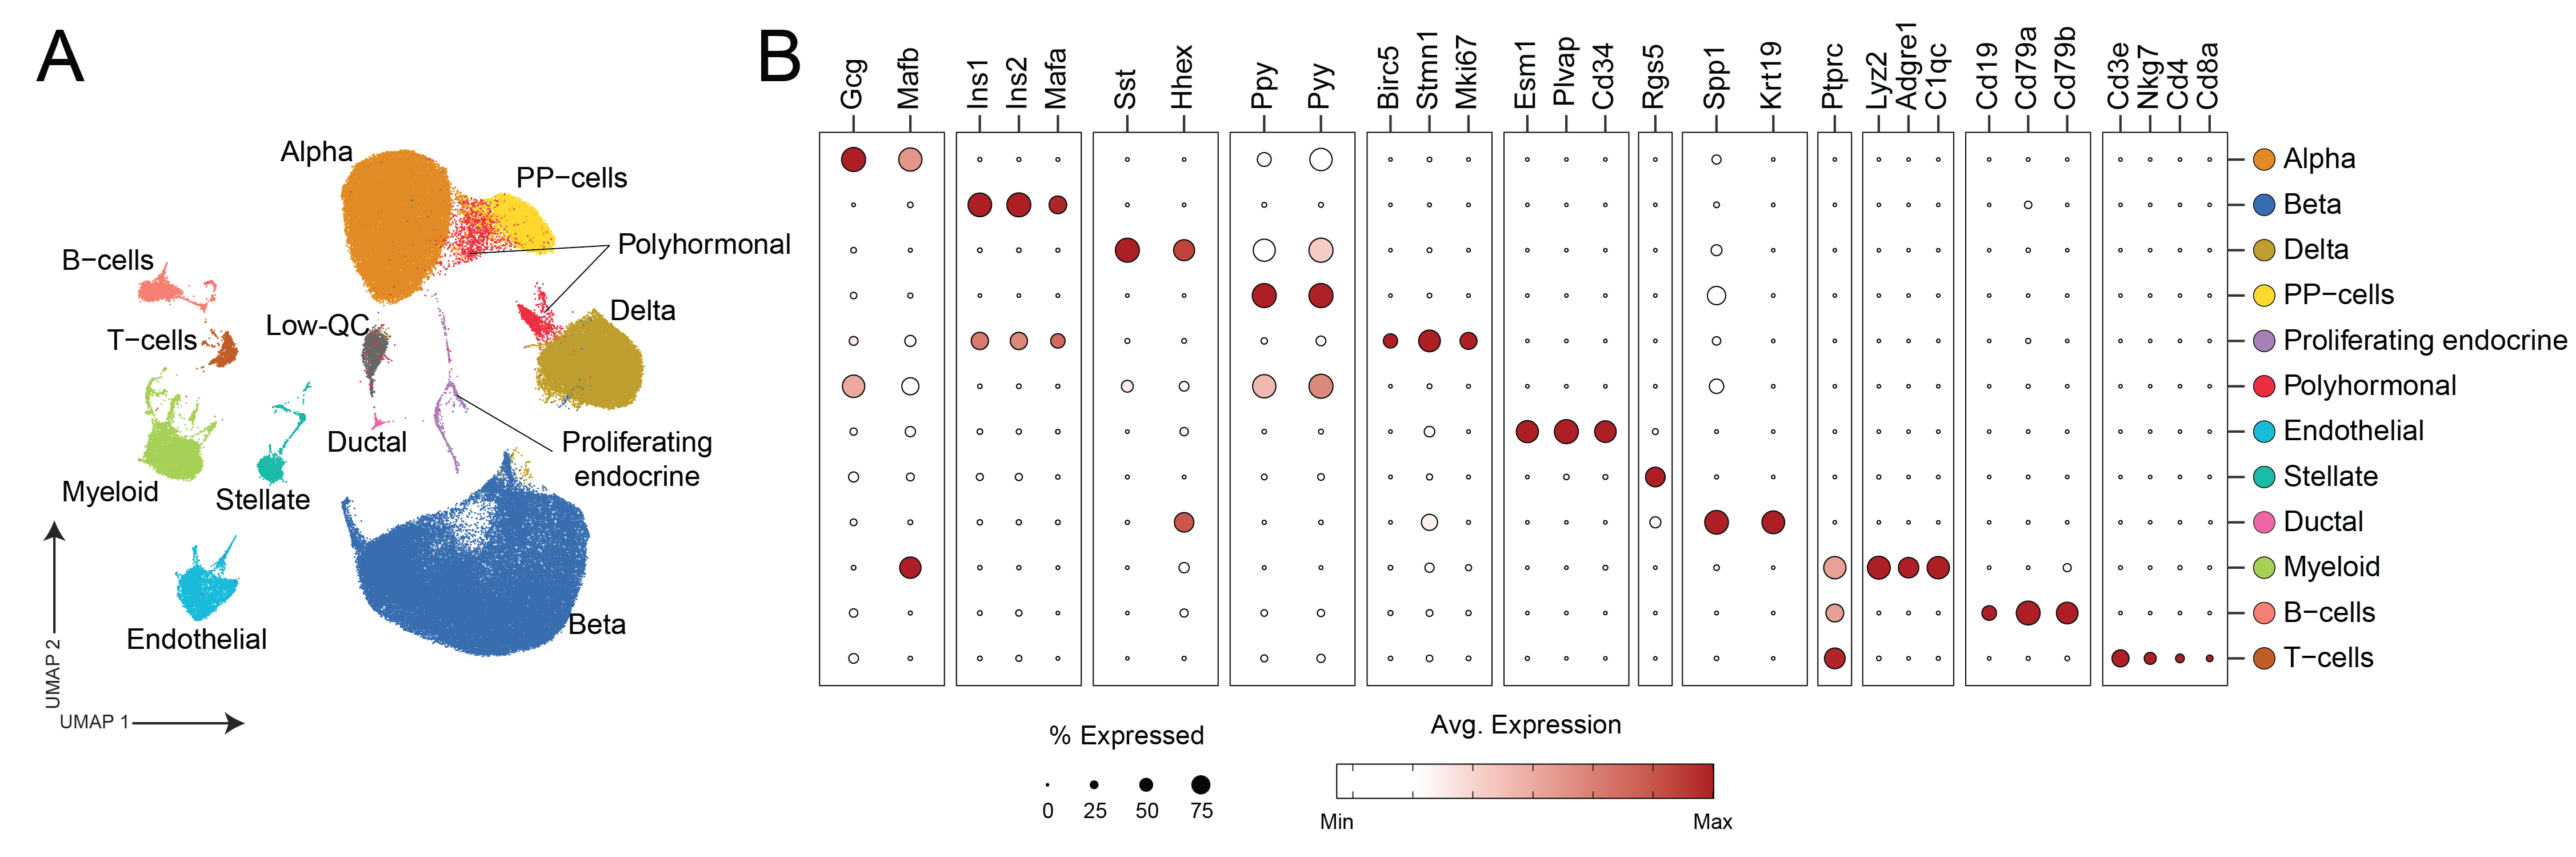
\includegraphics[width=\linewidth]{Chapter5/Fig/F3-2-v2-01.png}
\caption[Annotation of the full integrated dataset using marker genes]{\textbf{Integrated dataset of seven scRNA-seq studies across several models of β-cell decompensation and hyperglycemia.} \textbf{(A)} UMAP embedding of the integrated dataset depicting celltype annotations based on the expression of known markers. \textbf{(B)} UMAP embedding of the integrated dataset depicting the seven scRNA-seq studies. Datasets are described in Supplementary Table \ref{tab3-1}.}
\label{fig:3-2}
\end{figure}

This integrated embedding space showed clear separation into distinct clusters, which corresponded to distinct cell-types that originate from the different datasets \textbf{(Fig. \ref{fig:3-2} A)}. This provided empirical evidence that the previous step of data integration was indeed successful, thereby ensuring optimal trade-off between batch correction and biological conservation on the level of cell-types \textbf{(Fig. \ref{suppl_fig:chp3_study} A)}. The integrated dataset contains 124,191 cells across 16 samples \textbf{(Fig. \ref{suppl_fig:chp3_study} B, Supplementary Table \ref{tab:3-3})}. We manually annotated the four major islet cell-types using the expression of hormone markers: Alpha ($\alpha$) – \textit{Gcg}, Beta ($\beta$) - \textit{Ins1} and \textit{Ins2}, Delta ($\delta$) – \textit{Sst} and PP-cells ($\gamma$) – \textit{Ppy}. Apart from the major hormone secreting cell-types, we also annotated poly-hormonal cells expressing more than one hormone marker simultaneously. We identified the poly-hormonal cells by using a step-wise strategy of: \textbf{(i)} setting thresholds of hormone expression, \textbf{(ii)} identifying cells co-expressing any two hormone markers and \textbf{(iii)} referring to existing literature about poly-hormonal singlets and poly-hormonal doublets \textbf{\cite{sachs_targeted_2020, perez-frances_pancreatic_2021}}. Based on this, we were able to identify `Alpha-PP’ and `Delta-PP’ as the major poly-hormonal contributors and excluded `Alpha-Beta' and `Beta-Delta' as probable poly-hormonal doublets from further analysis. We were also able to identify non-endocrine cell-types such as Endothelial – \textit{Pecam1}, Immune – \textit{Ptprc}, Stellate – \textit{Rgs5} and Ductal – \textit{Krt19} \textbf{(Fig. \ref{fig:3-2} B)}.


\clearpage

\section{Clustering of pseudo-bulk \( \mathbf{\upbeta}\)-cells segregates hyperglycemic\\from normoglycemic samples}
\label{sec:chp3_pseudobulk}

To focus upon transcriptional changes in islet β-cells during compensation and failure, we subset β-cells for further analysis. We subset cells annotated as `Beta' and `Proliferating-Endocrine', performed additional QC to remove polyhormonal cells expressing non-β hormones (\textit{Gcg, Sst, Ppy}), retained the proliferating β-cells, and re-integrated across the seven studies \textbf{(Fig. \ref{fig:3-3} A, Supplementary Table \ref{tab:3-3})}. The re-integration of β-cells was necessary to account for any nested batch effects that might have been persistent across the studies. On the integrated embedding, the β-cells from the healthy controls employing adult mice and the 2 years old mice from Aging/maturation study overlapped with each other, whereas the cells from the experimental samples and the 3 wks old young mice, mapped together and away from the control groups \textbf{(Fig. \ref{suppl_fig:chp3_betastudy})}.\\\\
To provide a stringent assessment of the effectiveness of single-cell integration and to test whether the re-integration of β-cells was adequate for downstream analyses, we performed hierarchical clustering of samples based on the expression profiles of \textit{pseudobulk} β-cells. We aggregated the normalizd expression values of the 3000 \glspl{hvf} across all the experimental samples and the aggregated expression matrix was used to cluster genes into nine modules, grouping genes with similar expression profiles across the samples \textbf{(Fig. \ref{fig:3-3} B)}. Based on these gene modules, hierarchical clustering of the experimental samples separated the hyperglycemic models such as the insulin receptor blockade with S961, obese \textit{ob/ob} animals and partial β-cell ablation with \gls{stz} from their normoglycemic controls. However, these normal controls did not cluster with the healthy controls of the remaining studies likely due to enduring batch effects between the studies. The \textit{dbHet} animals of 6 and 9-weeks old clustered together and away from the \textit{db/db} cohorts, which also clustered together. Similarly, samples with mice fed chow diet for 1 or 12 weeks clustered together and away from the WD-fed counterparts of both time-points. Interestingly, the fasting and feeding samples from the Meal feeding study clustered together \textbf{(Fig. \ref{fig:3-3} B)}, reflecting the minimal effect of the feeding intervention on β-cell workload compared to models that exerted higher workloads on the β-cell.\\

%\clearpage

\begin{figure}[t]
\centering
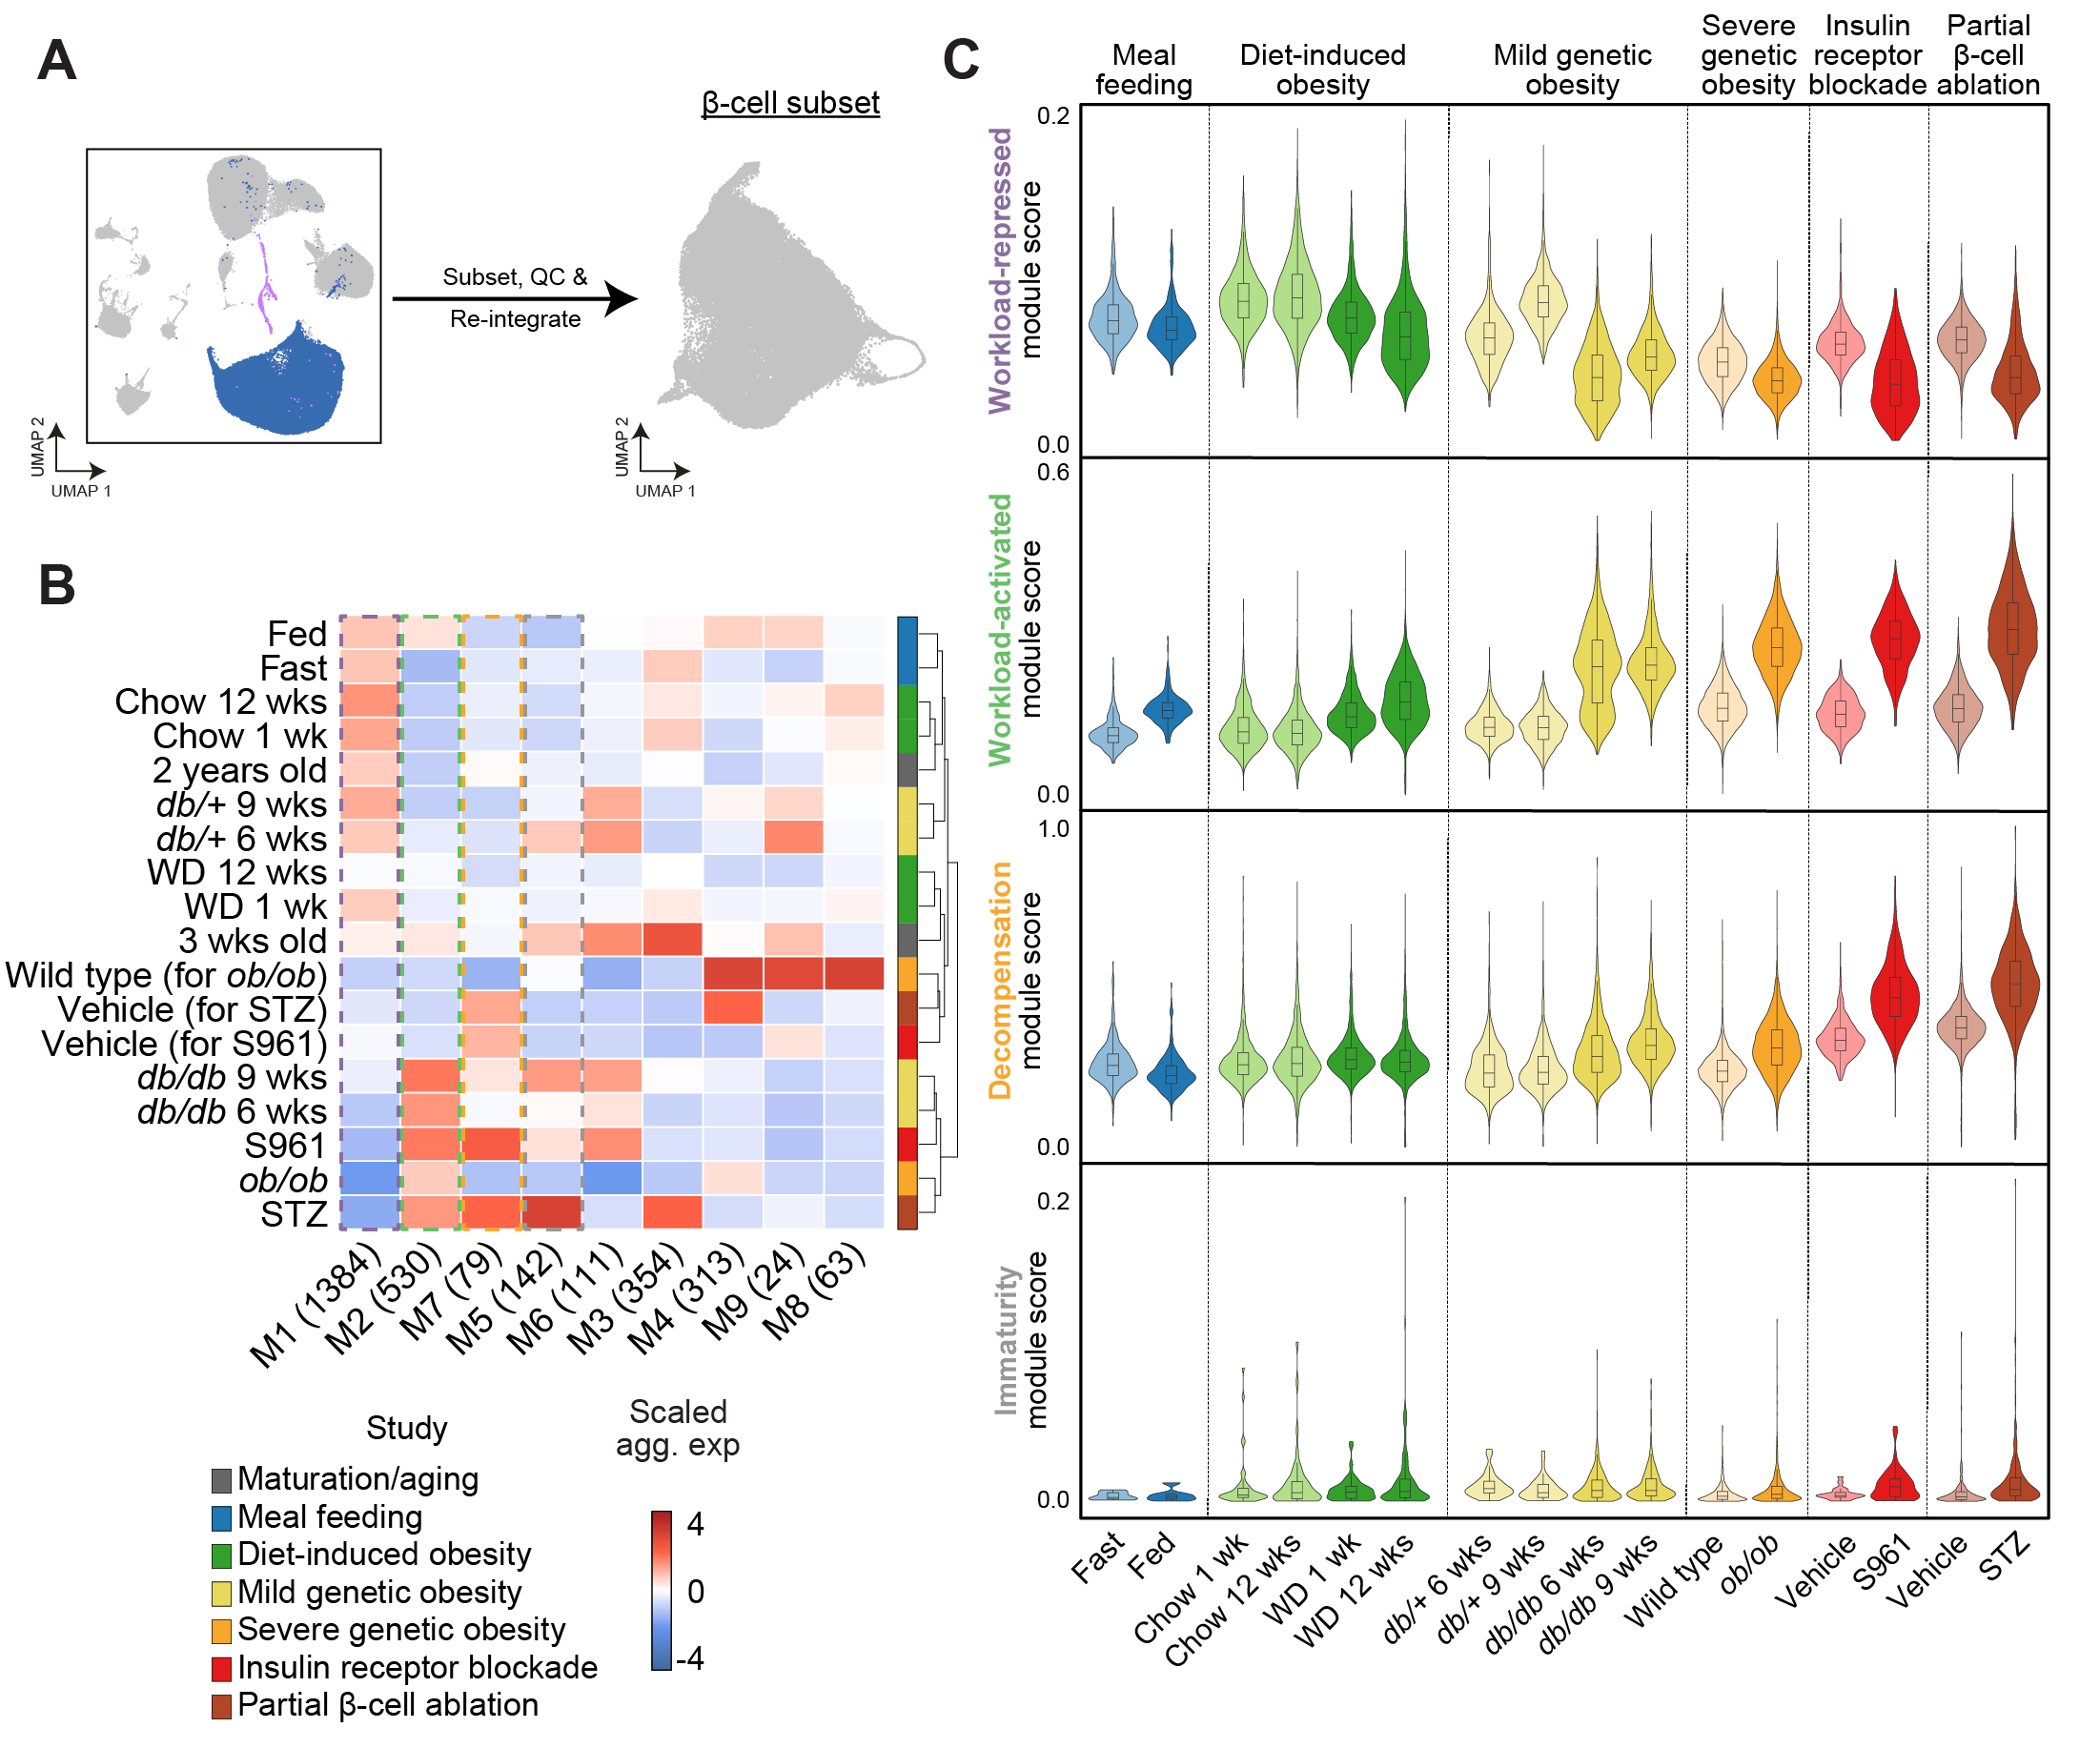
\includegraphics[width=\linewidth]{Chapter5/Fig/F3-3-01.png}
\caption[Hierarchical Clustering of pseudobulk β-cells across the samples]{\textbf{Hierarchical Clustering of pseudobulk β-cells across the samples.} \textbf{(A)} Heatmap depicting the hierarchical clustering of samples from seven studies based on the scaled aggregate expression of pseudobulk β-cells. The number of genes in each of the module is indicated in parantheses. \textbf{(B)} Violin plots depicting gene-set score of β-cells across all the samples from six studies for four modules highlighted in panel \textbf{A}. The Maturation/aging study is not depicted.}
\label{fig:3-3}
\end{figure}

We then performed gene-set scoring on a single-cell level for four modules (\textit{Modules M1,M2,M5} and \textit{M7}) identified from the hierarchical clustering of pseudobulk β-cells across the samples \textbf{(Fig. \ref{fig:3-3} C)}. Module \textit{M1} was repressed by all conditions of increased workload and contained known markers of β-cell function (\textit{Mafa, Slc2a2}) and development (\textit{Neurod1, Pdx1}) as well as ion homeostasis (\textit{Atp2a2, Trpm5}) and was termed as `Workload-repressed module' \textbf{(Fig. \ref{fig:3-3} C, \textit{top row})}. On the other hand, module \textit{M2} was activated in response to increased β-cell workload in models of mild (\textit{db/db}) and severe (\textit{ob/ob}) genetic obesity, insulin receptor blockade (S961) and partial β-cell ablation (\gls{stz}). The expression of this module was also slightly elevated in response to feeding as well as in the young 3 wks old mice. Module-2 associated with genes involved in protein processing in ER (\textit{Calr, Dnajb11, Hspa5}) and translation (\textit{Sec11a/c, Spcs1/2}). Therefore, we termed this module as ‘Workload-activated module’ \textbf{(Fig. \ref{fig:3-3} C, \textit{second row})}. In the \gls{mia} \textbf{\cite{hrovatin_delineating_2023}}, the authors identified three gene programs (GPs 2,3 and 4) which showed higher activity in the \textit{db/db + mSTZ} state and contained known diabetes markers or were associated with ER stress Based on the overlap of markers, the `Workload-activated' module identified here and GPs 2,3 and 4 from the \gls{mia} likely represent the same gene-set with genes up-regulated in response to increased β-cell workload. We also identified STZ-specific module \textit{M5}, which is likely similar to GPs 8 and 23 identified in \gls{mia}, associated with immaturity. Additionally, this analysis also revealed a ‘decompensatory’ profile (\textit{Module-7}), which characterized the insulin receptor blockade as well as the partial β-cell ablation models (S961+\gls{stz}) \textbf{(Fig. \ref{fig:3-3} C, \textit{third row})}. \hl{This module was comprised of ribosomal genes which were up-regulated in response to severe hyperglycemia due to S961 or STZ treatment. <need more characterization>}\\\\
In summary, the hierarchical clustering of pseudobulk β-cells provided further evidence for successful re-integration of β-cells from all experimental samples, distinguishing hyperglycemic models from normoglycemic control samples. In normoglycemic controls, samples from low-to-moderate β-cell workload models and severe hyperglycemic models clustered separately, likely due to enduring batch effects. Furthermore, this analysis identified gene-sets associated with increasing β-cell workload and with failure. This revealed that β-cell transcriptional signatures of workload-activated genes and hyperglycemia-repressed genes are similar across models.


\clearpage

%\section{Identification and classification of \( \mathbf{\upbeta} \)-cell subsets}
\section{Characterization of \( \mathbf{\upbeta} \)-cell heterogeneity using subset-\\enriched markers}
Classification of β-cell subsets based on
gene ontology analysis of subset-enriched mRNAs

\label{sec:chp3_betaclustering}
As previously discussed, extensive research has shown that β-cells are heterogeneous and this heterogeneity has been re-capitulated at a single-cell level. Independent analysis of the models used in this meta-analysis study identified distinct subtypes with transcriptomic differences relating to maturity and functional status of these β-cells. However, it is unclear how these subtypes relate to each other across several models of β-cell decompensation and failure. Therefore, in order to understand β-cell heterogeneity in a more unified framework and to understand how changes in β-cell workload and changes in glycemic dysregulation affect their transcriptomes, we classified β-cells into six putative subsets using unsupervised clustering \textbf{(Fig. \ref{fig:3-4} A)}. We then predicted cellular processes active in each cluster using GO and pathway analyses of marker genes associated with each cluster.\\\\
Markers expressed highest in β-1 cells were enriched for GOs and pathways such as `oxidative phosphorylation' and `regulation of insulin secretion', including previously described markers of β-cell maturity such as \textit{Mafa, Slc2a2}  and \textit{Ucn3}, and were therefore termed normal β-cells (\textbf{β-1 Normal}) \textbf{(Fig. \ref{fig:3-4} B,C)}. As expected, the β-1 cluster was enriched in the unchallenged controls of six studies (Meal feeding, Diet-induced obesity, Mild and Severe genetic obesity, Insulin receptor blockade and partial β-cell ablation) as well as in the 2 years old mice from the Aging/maturation model \textbf{(Fig. \ref{fig:3-4} D)}. The resemblance of β-cells from aged mice to the healthy and normal β-cells from younger mice has previously been demonstrated with aging improving pancreatic β-cell funciton in mice \textbf{\cite{xin_single-cell_2016}}. \\\\
On the opposite end of the spectrum, well-known markers of β-cell immaturity (e.g. \textit{Cd81} \textbf{\cite{salinno_cd81_2021}}, \textit{Fos, Jun})  were strongly expressed in a very minor subset of cells annotated as β-5 \textbf{(Fig. \ref{fig:3-4}B)}. The β-5 subset was enriched in the very young 3 wks old mice  \textbf{(Fig. \ref{fig:3-4}D)}, thereby suggesting that such an expression profile indicates that this minor subset is composed of developmentally immature β-cells that are yet to establish a mature identity. We therefore termed this subset as `β-5 Dev-immature'.
\clearpage

\begin{figure}[t]
\centering
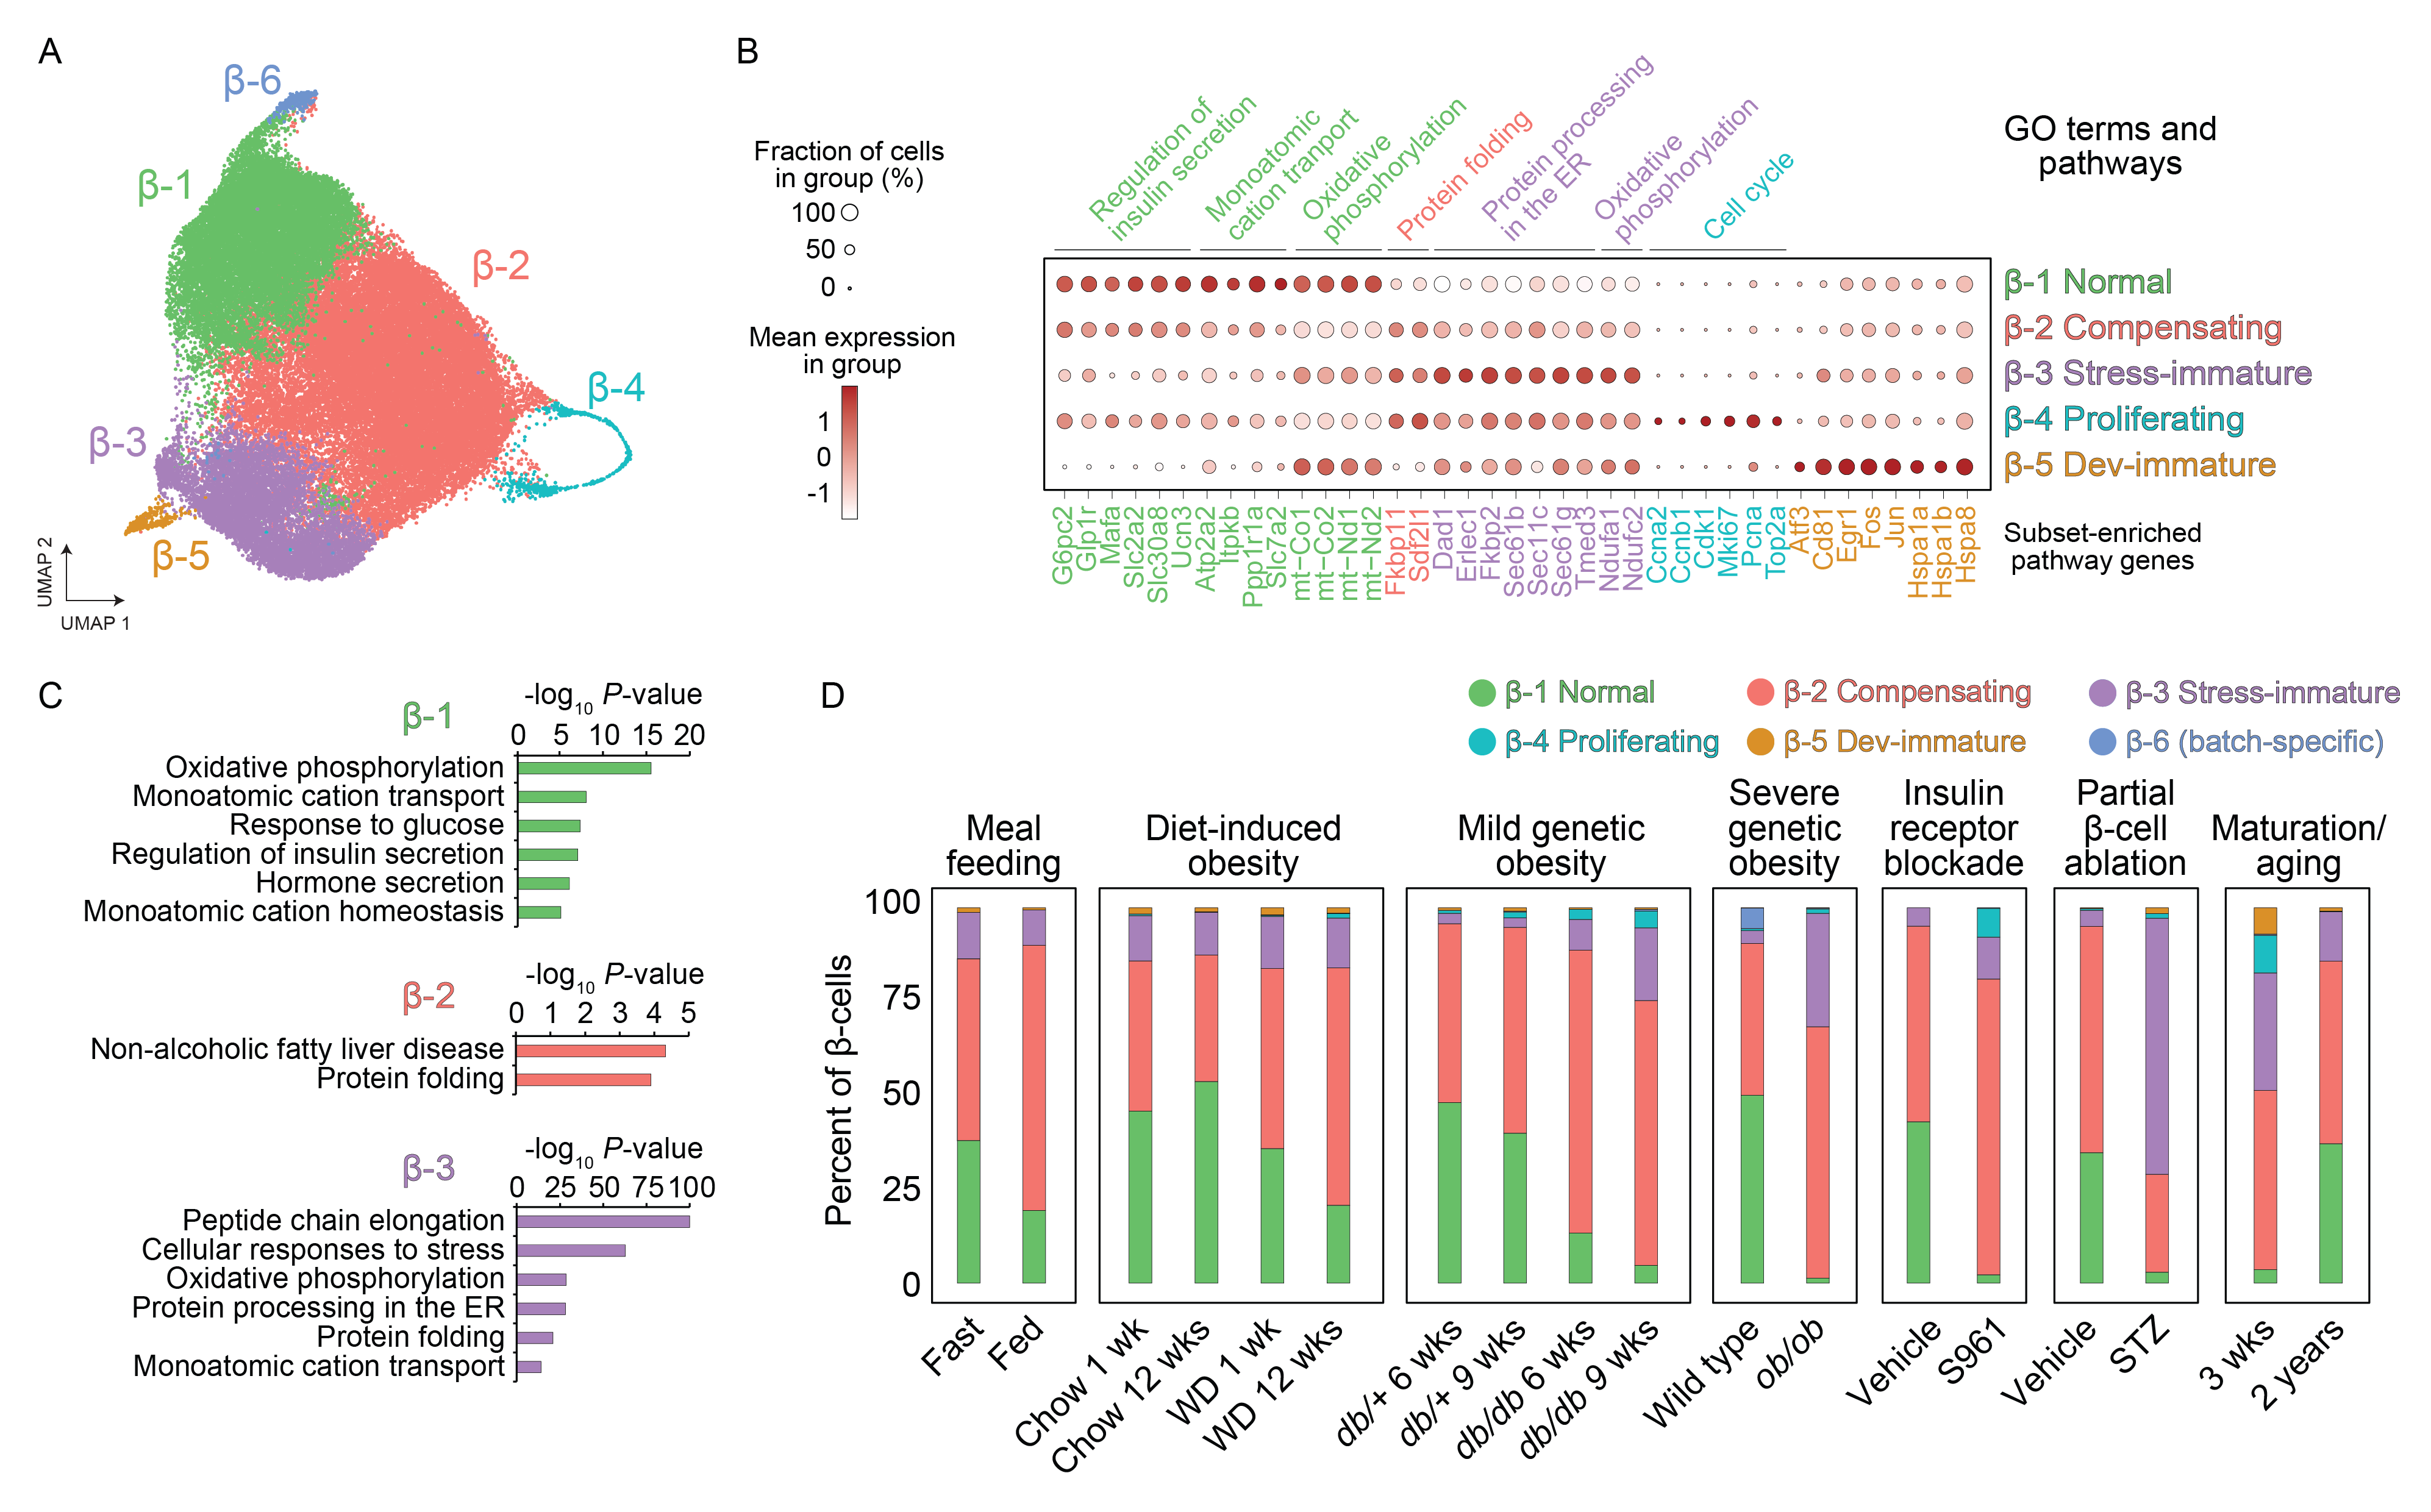
\includegraphics[width=\linewidth]{Chapter5/Fig/F3-1-v2-03.png}
\caption[Characterization of β-cell heterogeneity using subset-
enriched markers]{}
\label{fig:3-4}
\end{figure}

The β-3 subset was characterized by expression of genes enriched in the GO term `cellular responses to stress' \textbf{(Fig. \ref{fig:3-4} B,C)}. This subset was not enriched upon meal feeding compared to fasting control or by WD feeding for 1 or 12 weeks, wherein the proportion of β-3 cells were similar to the corresponding chow-fed controls. In models of hyperglycemia, the proportion of the β-3 subset was strongly expanded in challenged mice compared to their corresponding controls. This enrichment was strongest in the \gls{stz}-treated mice, which had the highest proportion of this cluster among all the other cohorts \textbf{(Fig. \ref{fig:3-4} D)}. This was also evident in the original study, in which the authors identified a β-immature state that becomes abundant in \gls{stz}-treated islets, and shows up-regulation of genes involved in ER stress and oxidative phosphorylation. This suggests that the β-3 subset likely resembles the β-mSTZ cells from \textbf{\cite{sachs_targeted_2020}} in transcriptional profile. Notably, the 3 wks old mice from the Maturation/aging study also depicted an enrichment of the β-3 subset compared to the aged 2-years-old mice. Additionally, both, the β-3 and β-5 subsets showed strong subset-specific mRNA expression of \textit{Cd81}, which has been established as a known marker of β-cell immaturity and dedifferentiation \textbf{\cite{salinno_cd81_2021}}. Thus, the early developmental stage seemed to go along with the enrichment of the β-3 subset with signs of stress-response and immaturity, in addition to the developmental immaturity associated with the β-5 subset. 
Based on these observations, we termed the β-3 subset as ‘\textbf{Stress-immature}’, as the dedifferentiation of β-cells in this subset can likely be attributed to the metabolic stress response of these cells under conditions of severe hyperglycemia (and insulin resistance).\\

Genes expressed most highly in the β-2 subset were enriched for the GO term `protein folding' mainly comprising genes encoding ER resident proteins including chaperones and prolyl isomerases \textbf{(Fig. \ref{fig:3-4} B,C)}. The up-regulation of ER machinery may signify an adaptive response to maintain ER homeostasis during increased requirements for insulin synthesis and processing during elevated β-cell workload. Genes overexpressed in β-2 cells tended to be expressed at intermediate levels in compared to β-1 or β-3 cells \textbf{(Fig. \ref{fig:3-4} B)}, and therefore β-2 associated genes were not as cluster-specific as genes characterizing β-1 or β-3 subsets. The β-2 subset constituted the largest proportion of β-cells and analysis of the composition of β-2 across the studies showed an almost universal enrichment of this subset with increasing β-cell workload \textbf{(Fig. \ref{fig:3-4} D)}. This included the `Meal feeding’ model, which involved a 4-hour window of feeding or additional fasting on the final day. This likely suggests that the composition shift of β-2 observed in fed animals compared to fasted controls is quite rapid and involves changes in cellular state, as this shift outpaces estimates of β-cell turnover that would be necessary to impact abundances of cellular subtypes. Similar enrichment of these β-2 `Compensating’ cells  were observed in the 1 and 12-week WD fed obese adult animals as well as the 6-week-old and 9-week-old \textit{db/db} mice, which are not yet hyperglycemic. The majority of the islets of the hyperglycemic \textit{ob/ob} mice and the S961-treated mice were composed of the β-2 compensating cells \textbf{(Fig. \ref{fig:3-4} D)}, again indicating the severity of the workload experienced by the β-cells in these models. Overall, the observed composition shifts suggest that increases in β-cell workload gives rise to a state switch from β-1 Normal to β-2 Compensating.\\


Apart from the three major β-cell clusters, the unsupervised clustering also identified three minor subsets: β-4 cells expressing genes enriched for the GO terms `cell cycle’ and `DNA metabolic process’ including established markers of β-cell proliferation (\textit{Mki67, Top2a}), 

\begin{figure}[b]
\centering
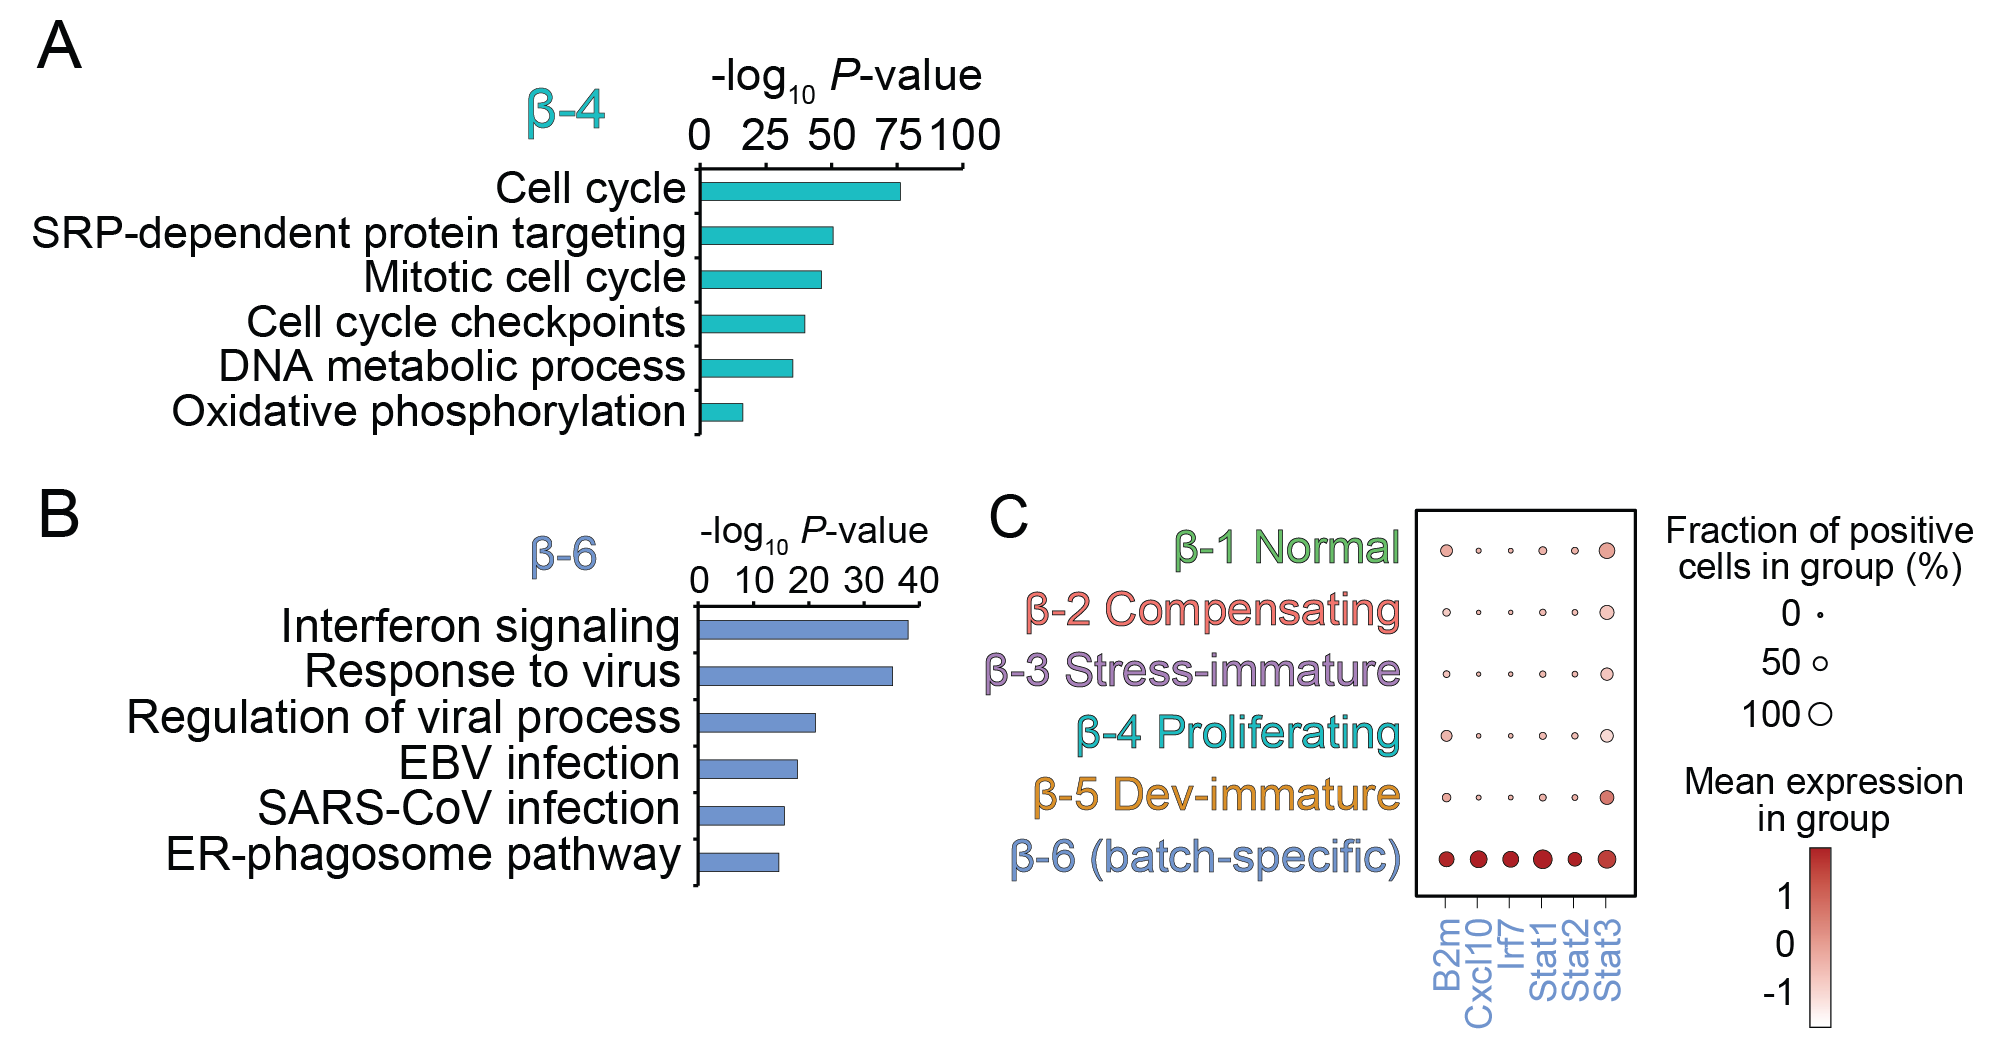
\includegraphics[width=12cm]{Appendix2/Fig/F3-1-v2-01.png}
\caption[Characterization of β-cell subsets using enriched markers and gene ontology]{}
\label{suppl_fig:chp3_betasubsets}
\end{figure}


which we termed ‘Proliferating’ cells \textbf{(Fig. \ref{fig:3-4} B, Fig. \ref{suppl_fig:chp3_betasubsets} A)}. These cells were enriched in the very young 3 wks old mice as well as the S961-treated animals, as expected \textbf{(Fig. \ref{fig:3-4} D)}. The proliferative nature of β-cells in response to increase in workload has been well documented \textbf{\cite{}}. Finally, β-6 comprised a minor subset, specific to the wild-type control for \textit{ob/ob} mice \textbf{(Fig. \ref{fig:3-4} D, Fig. \ref{suppl_fig:chp3_betasubsets} B,C)}; however, it is unclear what this small subset might represent. Of note, the gene module analysis identified module \textit{M8}, which was highly and specifically expressed in this sample \textbf{(Fig. \ref{fig:3-3} B)}, and the transcriptional profile of \textit{M8} was similar to GP25 in the \gls{mia}.\\

\begin{wrapfigure}{r}{0.6\textwidth}
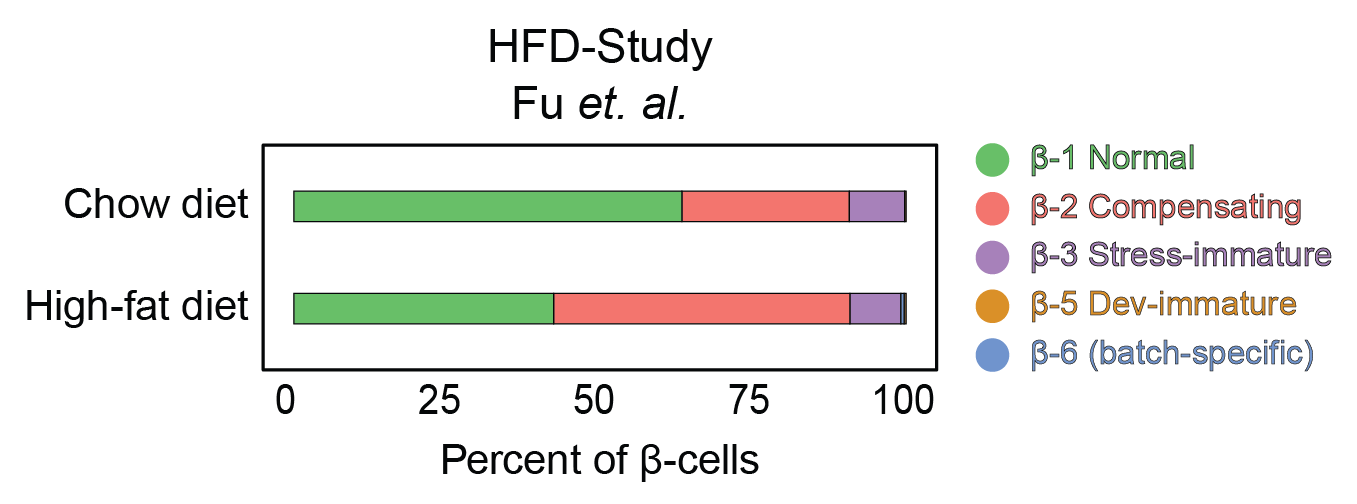
\includegraphics[width=9cm]{Chapter5/Fig/F3-1-v2-04.png}
\caption[PCA of Non-proliferating β-cell subsets]{Principal Component Analysis (\gls{pca}) of non-proliferating β-cells grouped by β-cell subsets across the first two \glspl{pc} (\gls{pc}1 and \gls{pc}2). The percentage of variance explained by each of the two \glspl{pc} are depicted in parentheses.}
\label{fig:chp3_hfdmapping}
\end{wrapfigure}


We also performed a comparative analysis by mapping an external, independent scRNA-seq study onto our integrated  β-cell subset. This dataset was obtained from islets from mice subjected to a high-fat diet (HFD) induced glucose intolerance \textbf{\cite{}}. We mapped the β-cells from this study onto our annotated β-cell subset, which enabled us to: \textbf{(i)} re-annotate the β-cells from the HFD-study with the subset annotations from the integrated atlas and \textbf{(ii)} compare the compositional changes of the β-cell subsets in response to a HFD-induced obesity model of metabolic stress. Similar to the WD-induced obesity after 1- or 12-weeks, a HFD feeding resulted in a subset composition shifts, with the proportion of β-1 Normal cells reduced after 8-weeks of HFD. This was accompanied by an increase in proportion of the β-2 Compensating subset in the HFD-fed mice. The proportion of β-3 subset remain unchanged between CD and HFD. The invariance of the β-3 Stress-immature subset in a mild-obesity model without hyperglycemia was also observed in our integrated atlas, in the case of Meal feeding or WD-induced obesity.\\


%\hl{<ERAD and UPR scores>}\\
In summary, unsupervised clustering of β-cells revealed six β-cell subsets which were annotated based on characteristic cellular processes of each of the subsets. We identified a normal β-cell cluster with known markers of maturity and function and a stressed β-cell cluster which depicted markers of stress response as well as immaturity. We additionally identified a small developmentally immature subset which can be distinguished from normal β-cells using previously described markers. Taken together, this likely suggests that β-cell immaturity can be associated with developmental or stress-response processes. The majority of β-cells were comprised of `decompensatory' nature, which showed an universal enrichment in response to increasing β-cell workload. Interestingly, this subset lacked any specific markers unlike β-1 or β-3, possibly suggesting that this subset likely corresponds to a β-cell state. Overall, this analysis revealed the heterogeneous landscape of β-cell transcriptome across several models of β-cell decompensation and hyperglycemia. 

\clearpage

\section{}
\label{sec:chp3_betaPCA}
In the above analyses, we identified three major β-cell subsets (β-1 Normal, β-2 Compensating and β-3 Stress-immature) with characteristic cellular processes and distinct compositional shifts during increasing β-cell workload. However, whether these subsets represent discrete subtypes or continuous states, and relationships between them is unclear. Additionally, as previously stated, since the over-expressed genes in the β-2 Compensating subset were not cluster-specific, compared to the β-1 or β-3 subsets, we hypothesized that the compensating state might be better represented by a continuous feature that distinguishes normal and compensating cells along a continuum. Therefore, to further assess the subset annotations of islet β-cells and their compositional shifts in response to increased workload in hyperglycaemic and insulin-resistant models, we utilized \gls{pca} of the re-integrated β-subset.\\


\begin{wrapfigure}{r}{0.5\textwidth}
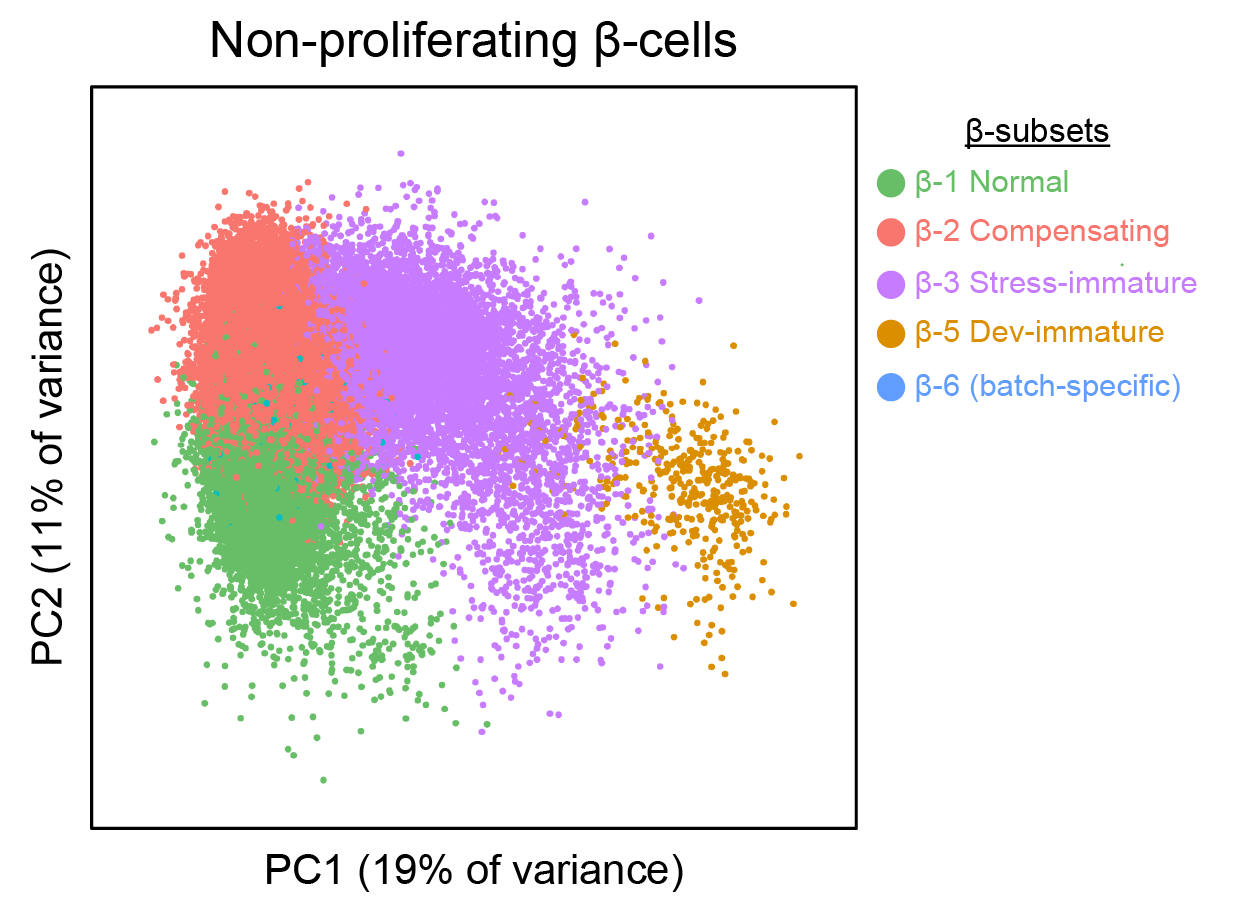
\includegraphics[width=8cm]{Chapter5/Fig/F3-6-01.png}
\caption[PCA of Non-proliferating β-cell subsets]{Principal Component Analysis (\gls{pca}) of non-proliferating β-cells grouped by β-cell subsets across the first two \glspl{pc} (\gls{pc}1 and \gls{pc}2). The percentage of variance explained by each of the two \glspl{pc} are depicted in parentheses.}
\label{fig:3-5}
\end{wrapfigure}


In theory, each principal component (\gls{pc}) represents an axis in a high-dimensional space that captures the largest amount of variation in the data. Thus, the first \gls{pc} is such that it maximizes this variance, the second \gls{pc} captures most of the remaining amount of variation and is orthogonal to the first \gls{pc}. In this way, the top \glspl{pc} are supposed to capture the most dominant factors of heterogeneity in the dataset, In the context of scRNA-seq, it is widely assumed that biological processes affect multiple genes in a coordinated manner whereas random or biological noise would affect each gene independently. %\st{Therefore, the earlier PCs are more likely represent the biological heterogeneity whereas the technical variability would be attributed with later PCs.}
Therefore, it is common practice in scRNA-seq to make use of earlier and top PCs in downstream analysis. This is a simple, highly-effective and widely used strategy in several fields.\\\\

We recomputed the \glspl{pc} for all the non-proliferating β-cells in our re-integrated subset. In our analysis, the first two \glspl{pc} (\gls{pc}1 and \gls{pc}2) were able to distinguish the three major β-cell subsets \textbf{(Fig. \ref{fig:3-5})}. Across the 3000 HVFs, \gls{pc}1 accounted for 19\% of the variance \textbf{(Fig. \ref{fig:3-5})} and corresponded with β-cell maturation state \textbf{(Fig. \ref{fig:3-6}, Fig. \ref{suppl_fig:chp3_pc1})}. This was evident from a histogram plot depicting cell densities along PC1 weights along with which the cells were ordered. Traversing along this `ranked axis’,we observed  that the higher density was accounted by the β-3 Stress-immature subset \textbf{(Fig. \ref{fig:3-6} A)} and β-5 Dev-immature subset \textbf{(Fig. \ref{suppl_fig:chp3_pc1} A)} and thereby distinguishing them from β-1 Normal or β-2 Compensating subsets.


\begin{figure}[H]
\centering
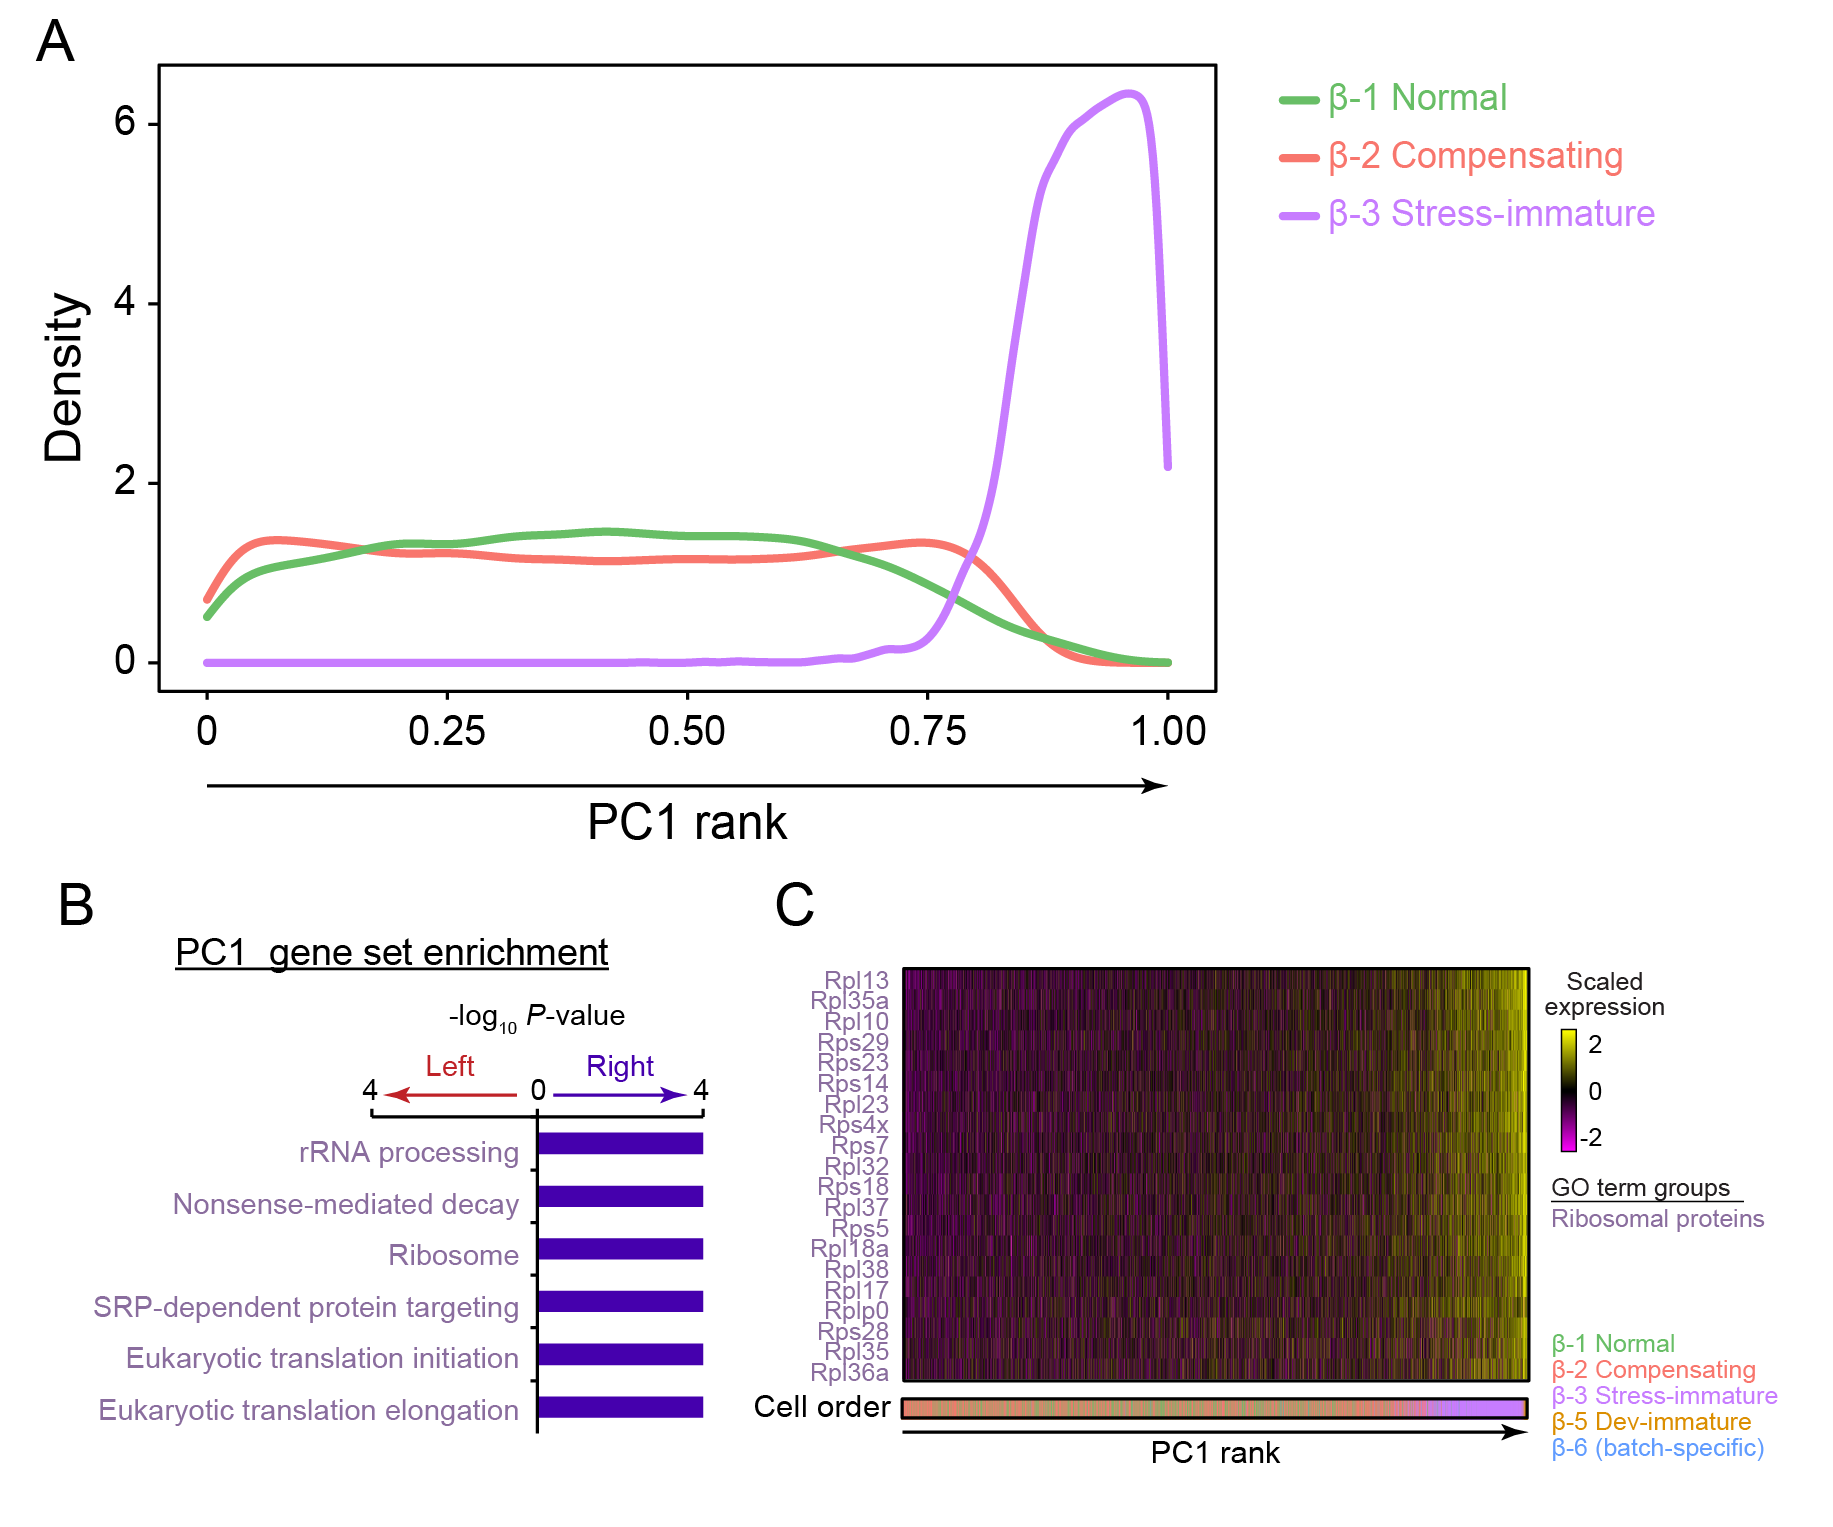
\includegraphics[width=\linewidth]{Chapter5/Fig/F3-6-02}
\caption[Deteriorating glucose homeostasis associates with PC1]{\textbf{Deteriorating glucose homeostasis associates with PC1}\\}
\label{fig:chp3_pc1}
\end{figure}


A shifted distribution of cells along PC1 across the experimental interventions depicted that the loss of β-cell maturity occurred in models with systemic hyperglycemia i.e., in \textit{ob/ob} mice and following S961- or \gls{stz}-treatment \textbf{(Fig. \ref{suppl_fig:chp3_pc1} B, \textit{bottom row})}. This was in contrast to the modest interventions which resulted in successful β-cell adaptation, wherein there were minor differences surrounding β-cell immaturity in feeding, WD-induced obesity or the \textit{db/db} mice \textbf{(Fig. \ref{suppl_fig:chp3_pc1} B, \textit{top row})}. Overall, this observation supports that β-cell decompensation associates with loss of maturity. In addition to the up-regulation of genes involved in OxPhos and protein processing in the ER in β-3 and β-5 subsets \textbf{(Fig. \ref{fig:3-4} B)}, \gls{pc}1 also corresponded with the up-regulation of ribosomal protein genes \textbf{(Fig. \ref{fig:3-6} B,C)}.\\ %\st{This could be explained by a higher demand for protein synthesis in β-3 subset in order to adapt to increased workload demands associated with hyperglycaemic environment and β-5 subset wherein cells could be producing a large number of ribosomes in order to support the synthesis of proteins required for maturation.}\\


%\clearpage

On the other hand, \gls{pc}2 explained 12\% of the variance across β-cell subsets \textbf{(Fig. \ref{fig:3-5})} and corresponded with increased insulin demand per β-cell \textbf{(Fig. \ref{fig:3-7}, Fig. \ref{suppl_fig:chp3_pc2})}. The ‘ranked’ histogram plot of the cells ordered by their PC2 weights distinguished β-1 Normal cells from β-2 or β-3 subsets. Further, the cell distributions across the PC2 rank was shifted for all experimental interventions, including fasting and refeeding. Thus, PC2 seemed to describe the extent of workload with respect to any model that increased insulin demand on a per β-cell basis, which can be impacted through either altered insulin sensitivity or altered β-cell numbers. Compared to PC1, diverse gene-sets were associated with PC2 progression with the apparent repression of mitochondrially-encoded components of the electron transport chain (ETC) and up-regulation of genes involved in proteostasis and the glycosylation machinery. We speculate these changes reflect activation of a program intended to preserve ER homeostasis when each cell is attempting to produce and secrete increasing amounts of insulin.\\

\begin{figure}[H]
\centering
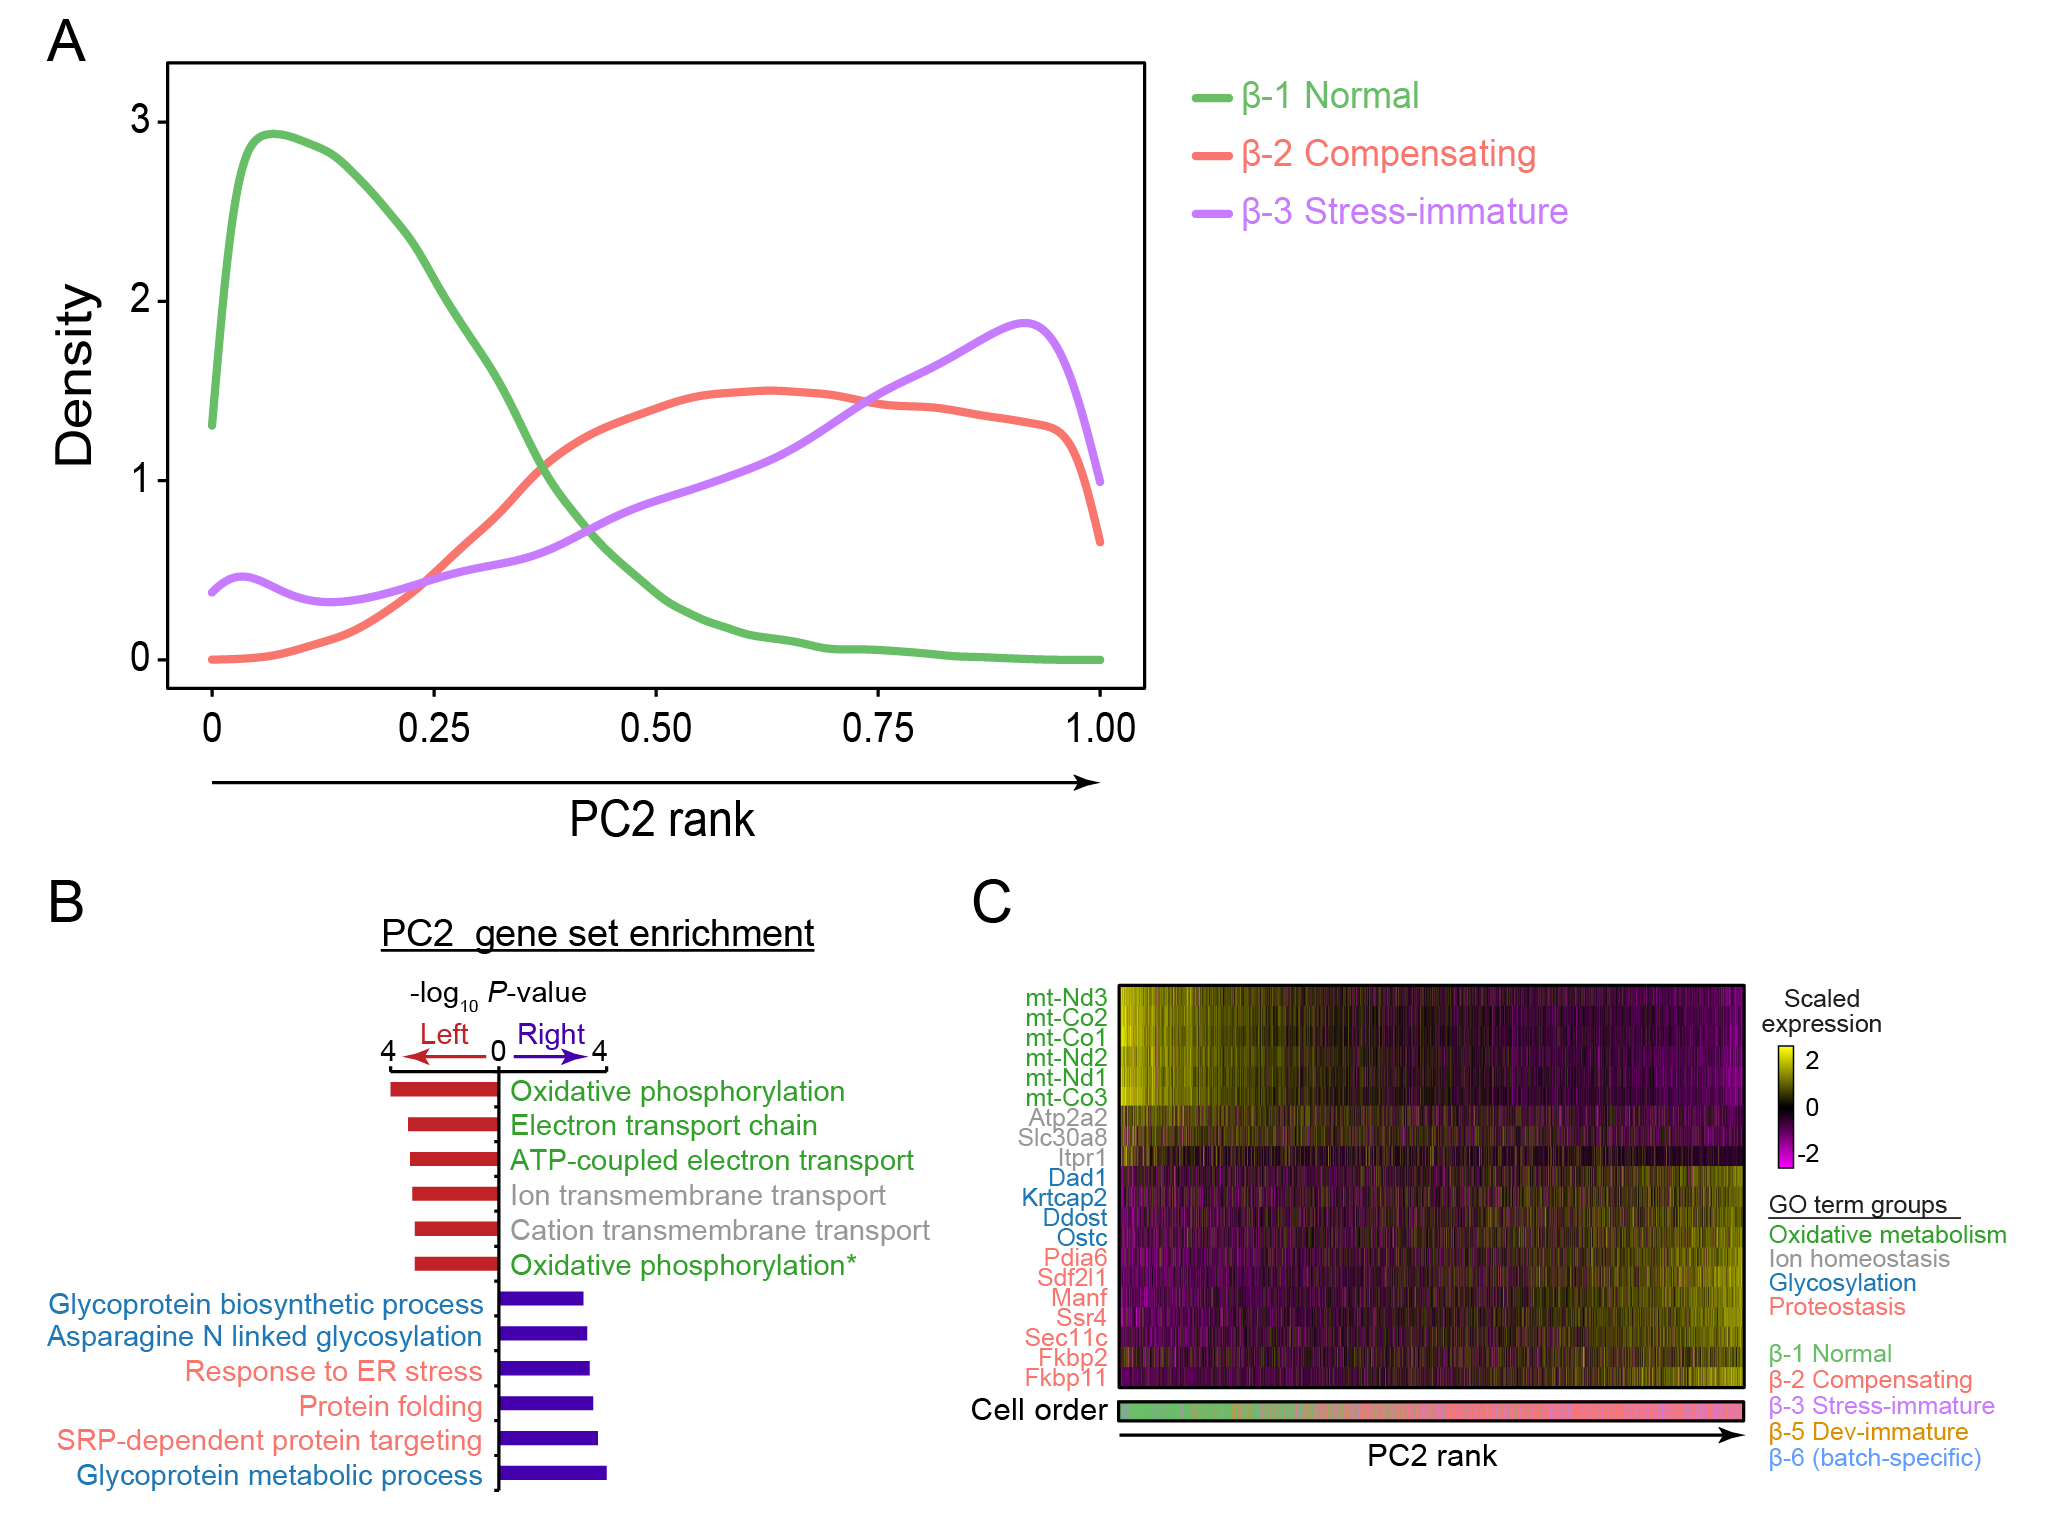
\includegraphics[width=\linewidth]{Chapter5/Fig/F3-6-03}
\caption[Increased β-cell workload associates with PC2]{\textbf{Increased β-cell workload associates with PC2}\\}
\label{fig:3-7}
\end{figure}

\clearpage

% \begin{wrapfigure}{l}{0.7\textwidth}
% 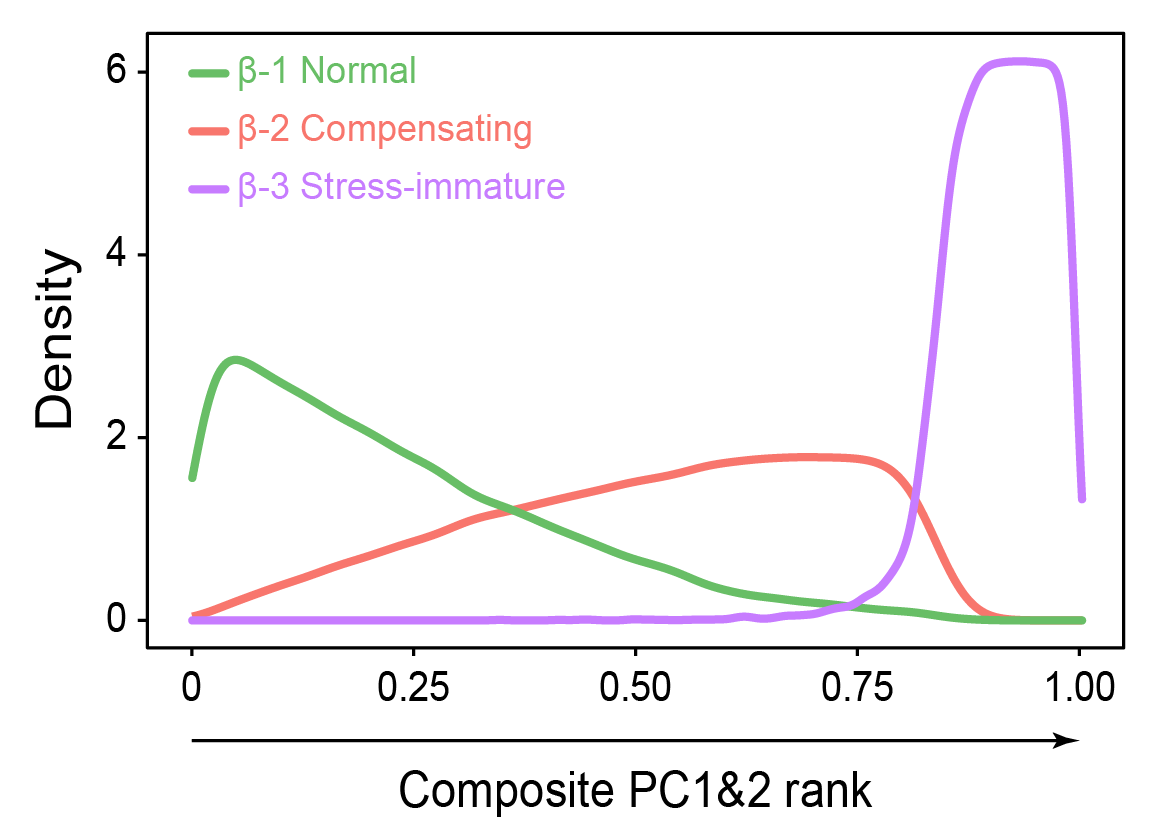
\includegraphics[width=10cm]{Chapter5/Fig/F3-6-04.png}
% \caption[Composite PC1 \& PC2]{}
% \label{fig:3-8}
% \end{wrapfigure}



Combining PC1 and PC2, we hypothesized that the three major subsets could be better represented along a composite axis that encompasses a degree of maturity (PC1) and a degree of workload (PC2). The β-1 Normal subset progressively switches to β-2 Compensating subset along the Maturity-Workload axis, therefore indicating that β-1 and β-2 could rather be continuous phenotypes as opposed to two discrete subsets. β-2 Compensating cells exhibit signatures of increased workload but still retain β-cell identity. β-3 Stress-Immature subset, on the other hand, are exposed to increased insulin demand and also lose their mature identity, thereby distinguishing these cells which are in a decompensated state, resulting in hyperglycemic phenotypes.


\mysidecaption{0.4}{%
\captionof{figure}[Trajectory of β-cell failure along PC1 and PC2]{\textbf{β-cell failure corresponds to increased workload concomitant with loss of maturation}}%
}
{%
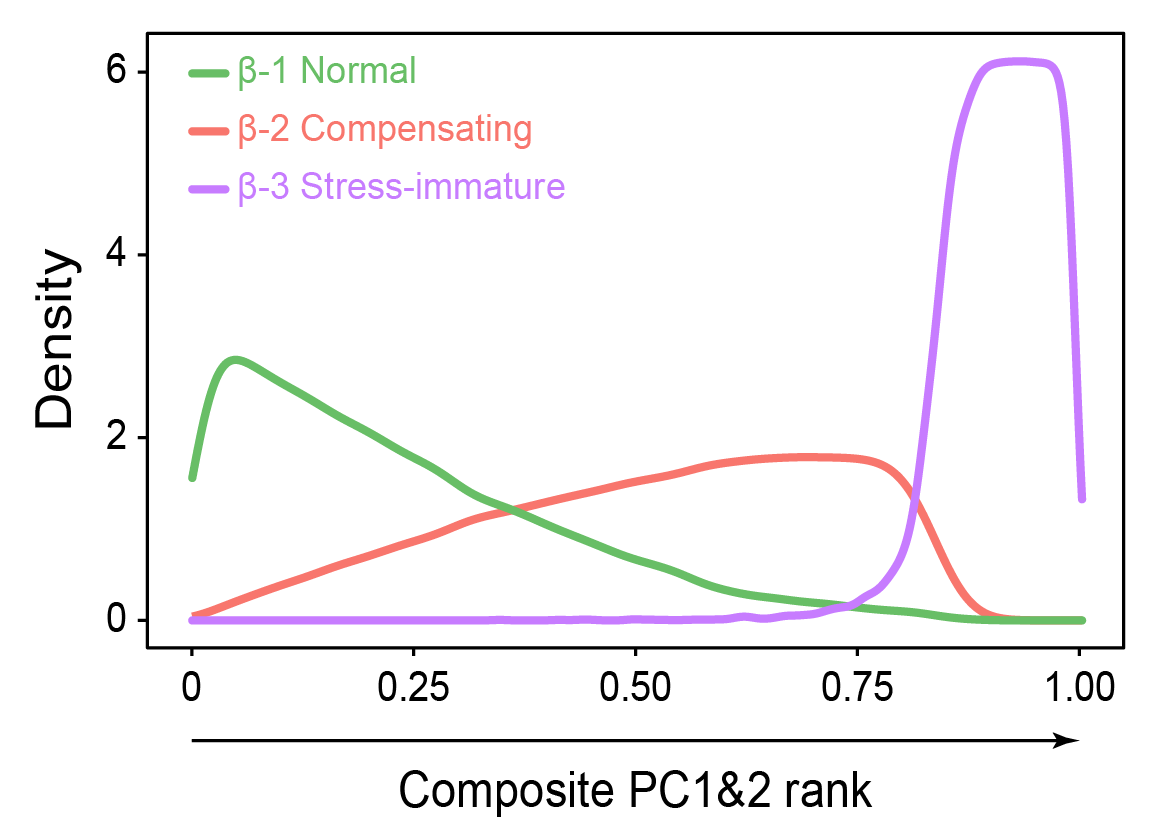
\includegraphics[width=9cm,height=9cm,keepaspectratio]{Chapter5/Fig/F3-6-04.png}%
}[t]%

\hl{\\\\In summary ...}

\clearpage

\section{Gene regulatory networks underlying the transcriptional\\heterogeneity of \( \mathbf{\upbeta} \)-cell subsets}
\label{sec:chp3_betaGRN}
Unraveling the complex web of \glspl{grn} is fundamental to decoding the complex regulatory mechanisms that govern cellular response to environmental cues. As already discussed, the development and maturation of β-cells is tightly regulated by the coordinated activity of several key \glspl{tf} (\textit{Pdx1, Mafa} and \textit{Nkx6-1}), that target several genes, in order to maintain normal β-cell identity and function. However, very little know is about how \glspl{tf} in β-cells are affected in response to increasing workload, and how they govern state transitions in an interconnected, heterogeneous manifold. Therefore, to understand the molecular mechanisms that underlie these transcriptional differences, we performed \gls{grn} analysis using pySCENIC to infer \gls{tf} activity and infer \gls{tf}-specific \glspl{grn}.\\ %A description of the workflow for \gls{grn} inference using the SCENINC workflow can be found in \hyperref[sec:scrna_analysis_grn]{Section 1.5.6}.\\

\begin{wrapfigure}{l}{0.5\textwidth}
%\centering
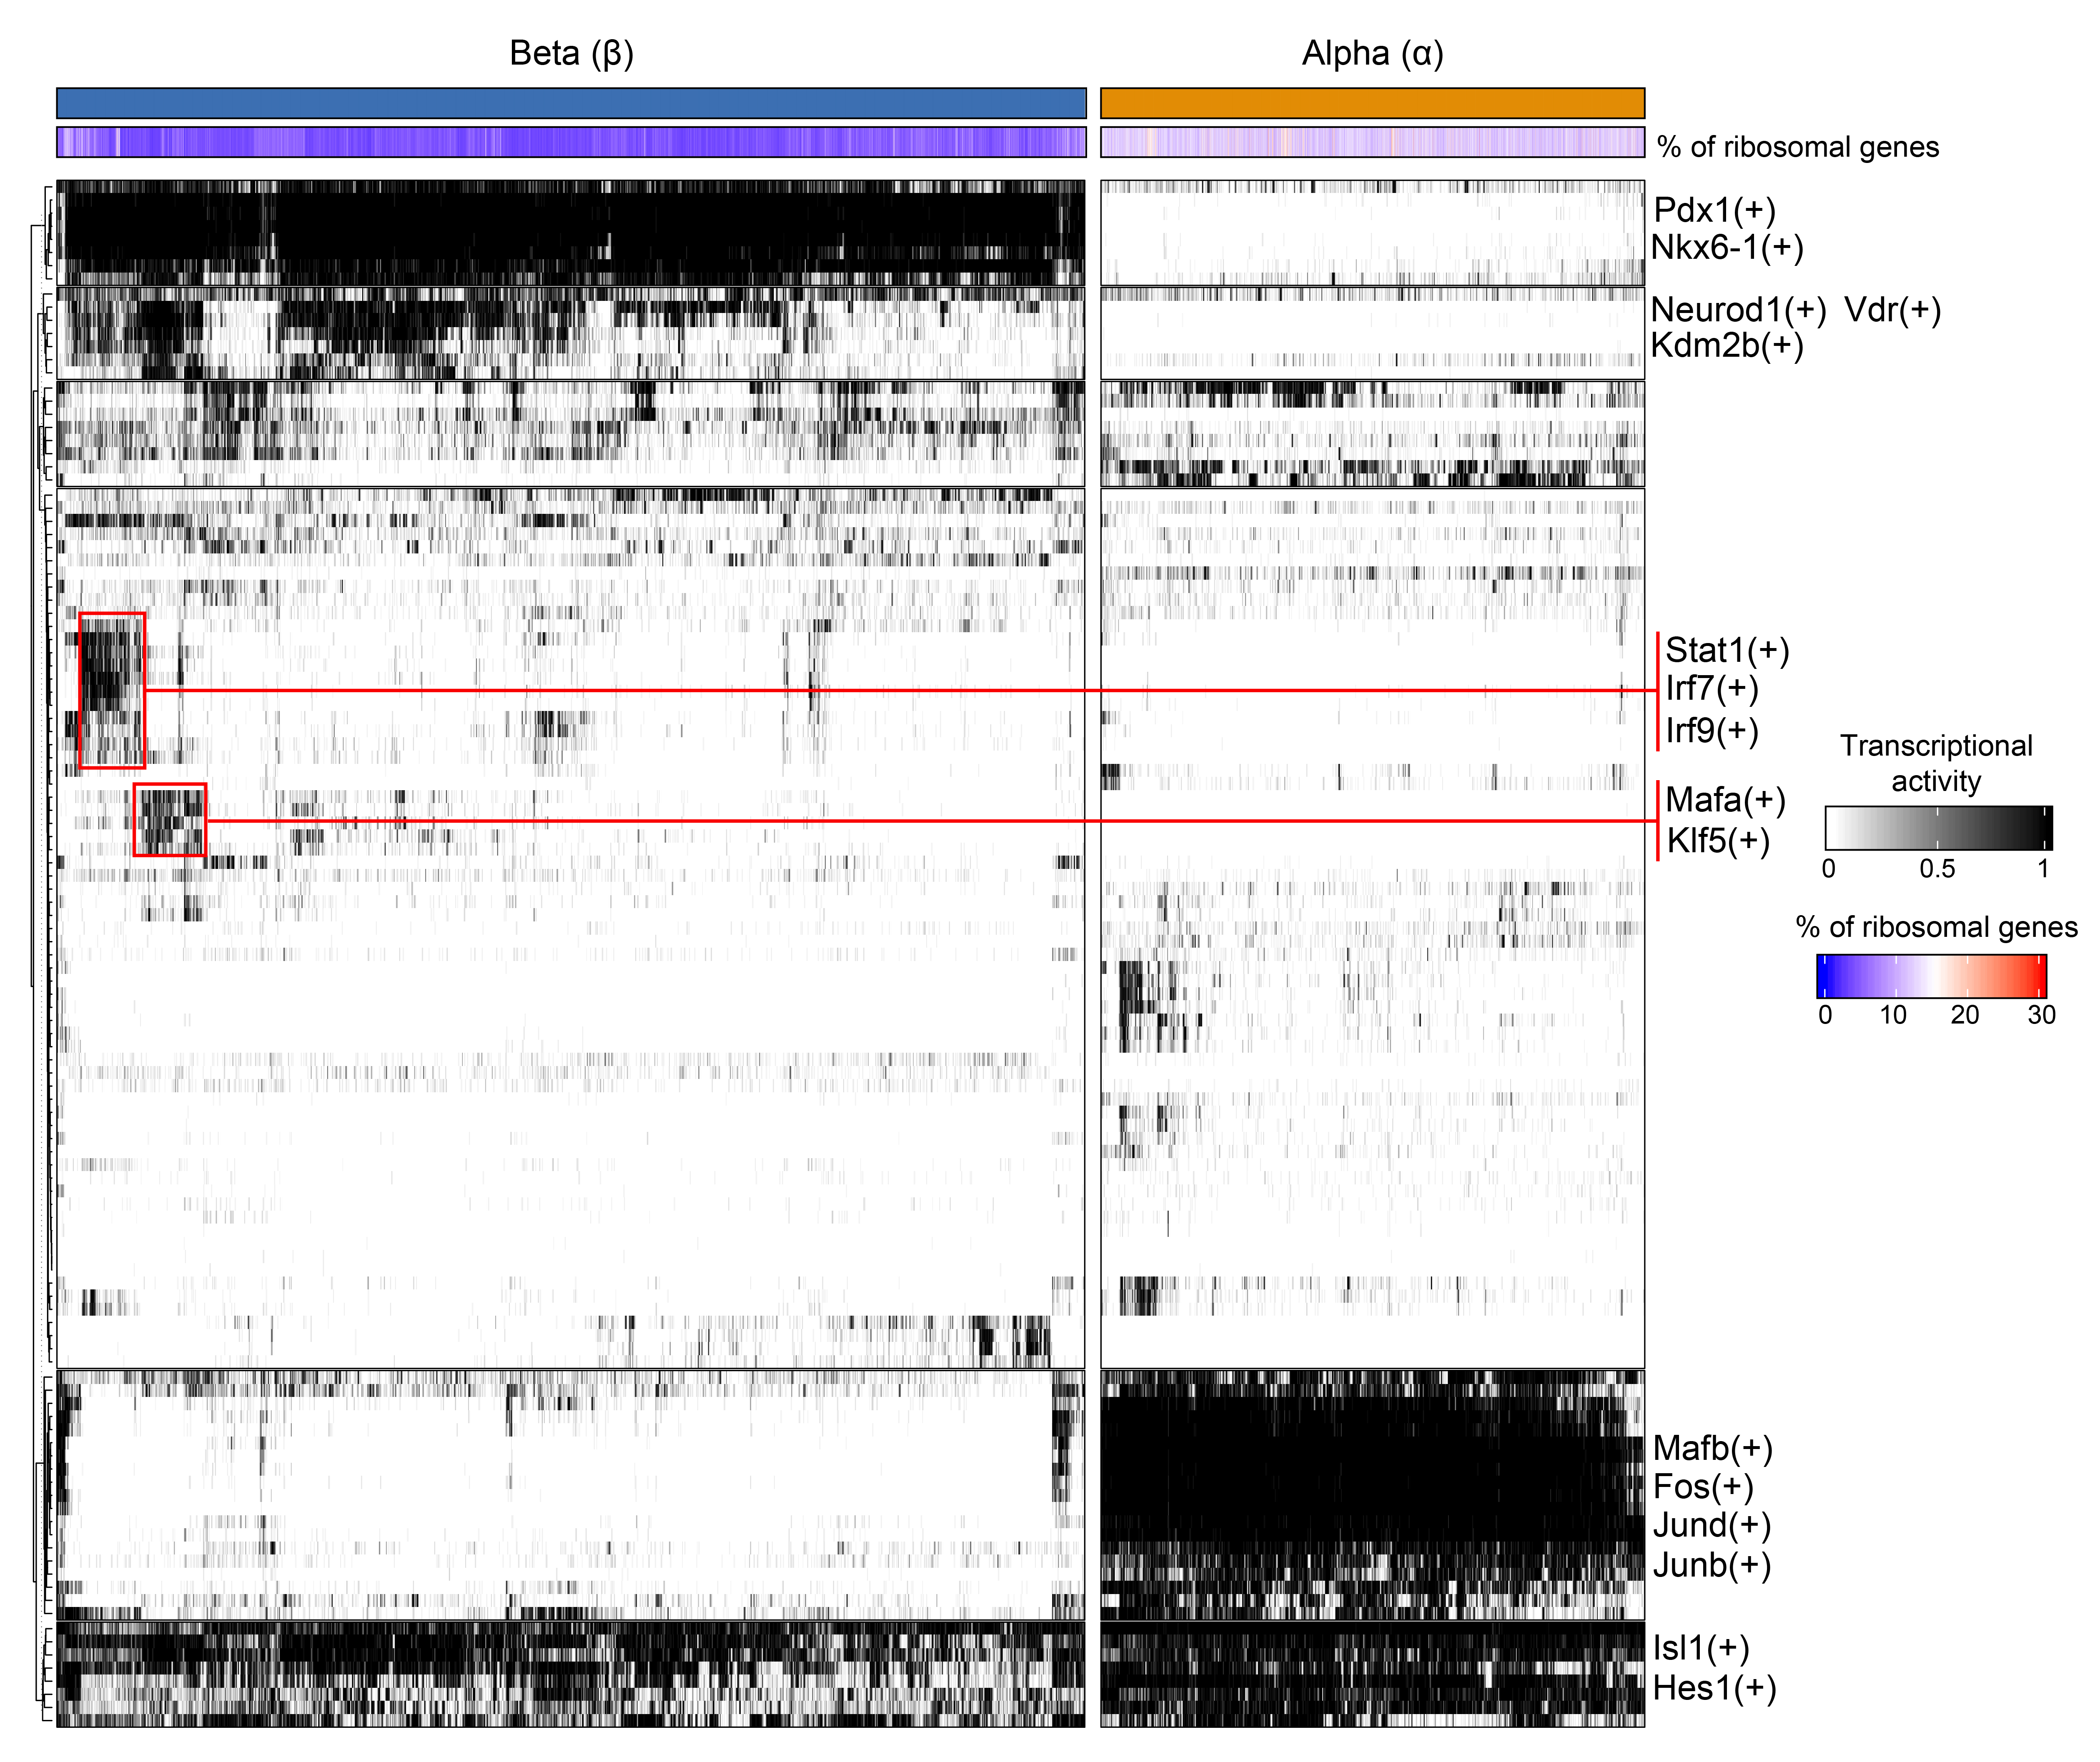
\includegraphics[width=8cm]{Chapter5/Fig/F3-11-01.png}
\caption[Identification of cell-type specific regulons]{\textbf{Identification of cell-type specific regulons.} Heatmap depicting the binarized AUC scores, representing the transcriptional activity of regulons across all the cells. Regulons shown in black are considered "ON", while regulons in white are considered "OFF". Top row shows the distribution of cells in the heatmap subdivided by cell-type and percentage of ribosomal genes.}
\label{fig:chp3_scenic-1}
\end{wrapfigure}

\par We applied pySCENIC to the two largest islet cell-types in our data: Alpha ($\alpha$) and Beta ($\beta$). We subsetted cells annotated as `Alpha' in the full integrated data \textbf{(Fig. \ref{fig:3-2} A)} and re-integrated this subset with the non-proliferating β-cells. We then applied pySCENIC to the Alpha-Beta re-integrated subset in order to identify α-cell and β-cell specific regulons \textbf{(Fig. \ref{fig:chp3_scenic_alphabeta})}. As expected, we identified \textit{Pdx1, Nkx6-1 and Mafa} regulons in β-cells and the \textit{Mafb} regulon in α-cells. We found the \textit{Isl1} regulon to be active in both cell-types, which is regarded as a candidate \gls{tf} regulator in islet cell lineage \textbf{\cite{juhl_mouse_2008}} and controls pancreatic α-cell fate and β-cell maturation \textbf{\cite{bohuslavova_isl1_2023}}. In addition, the \gls{tf} \textit{Hes1}, a downstream target of \textit{Notch} \textbf{\cite{hashemitabar_redefining_2019}}, was also active in both the cell-types.
\clearpage 
In β-cells, we identified 124 regulons across the five non-proliferating subsets. \glspl{tf} often work in coordination to regulate gene expression levels. Therefore, to determine the degree of TF activity coordination in mouse β-cells, we computed the connection specificity index (CSI) on the basis of pairwise comparisons of regulon activity patterns across cells, and identified five modules with varying number of regulons \textbf{(Fig. \ref{fig:3-10} A, Supplementary Table \ref{tab3-2})}. We also visualized the transcriptional \gls{grn} underlying the non-proliferating β-cells by using the top 1\% of the reported \gls{tf}-target associations based on the importance metric (IM) from the pySCENIC analysis \textbf{(Fig. \ref{fig:3-10} B)}.\\

\begin{figure}[H]
\centering
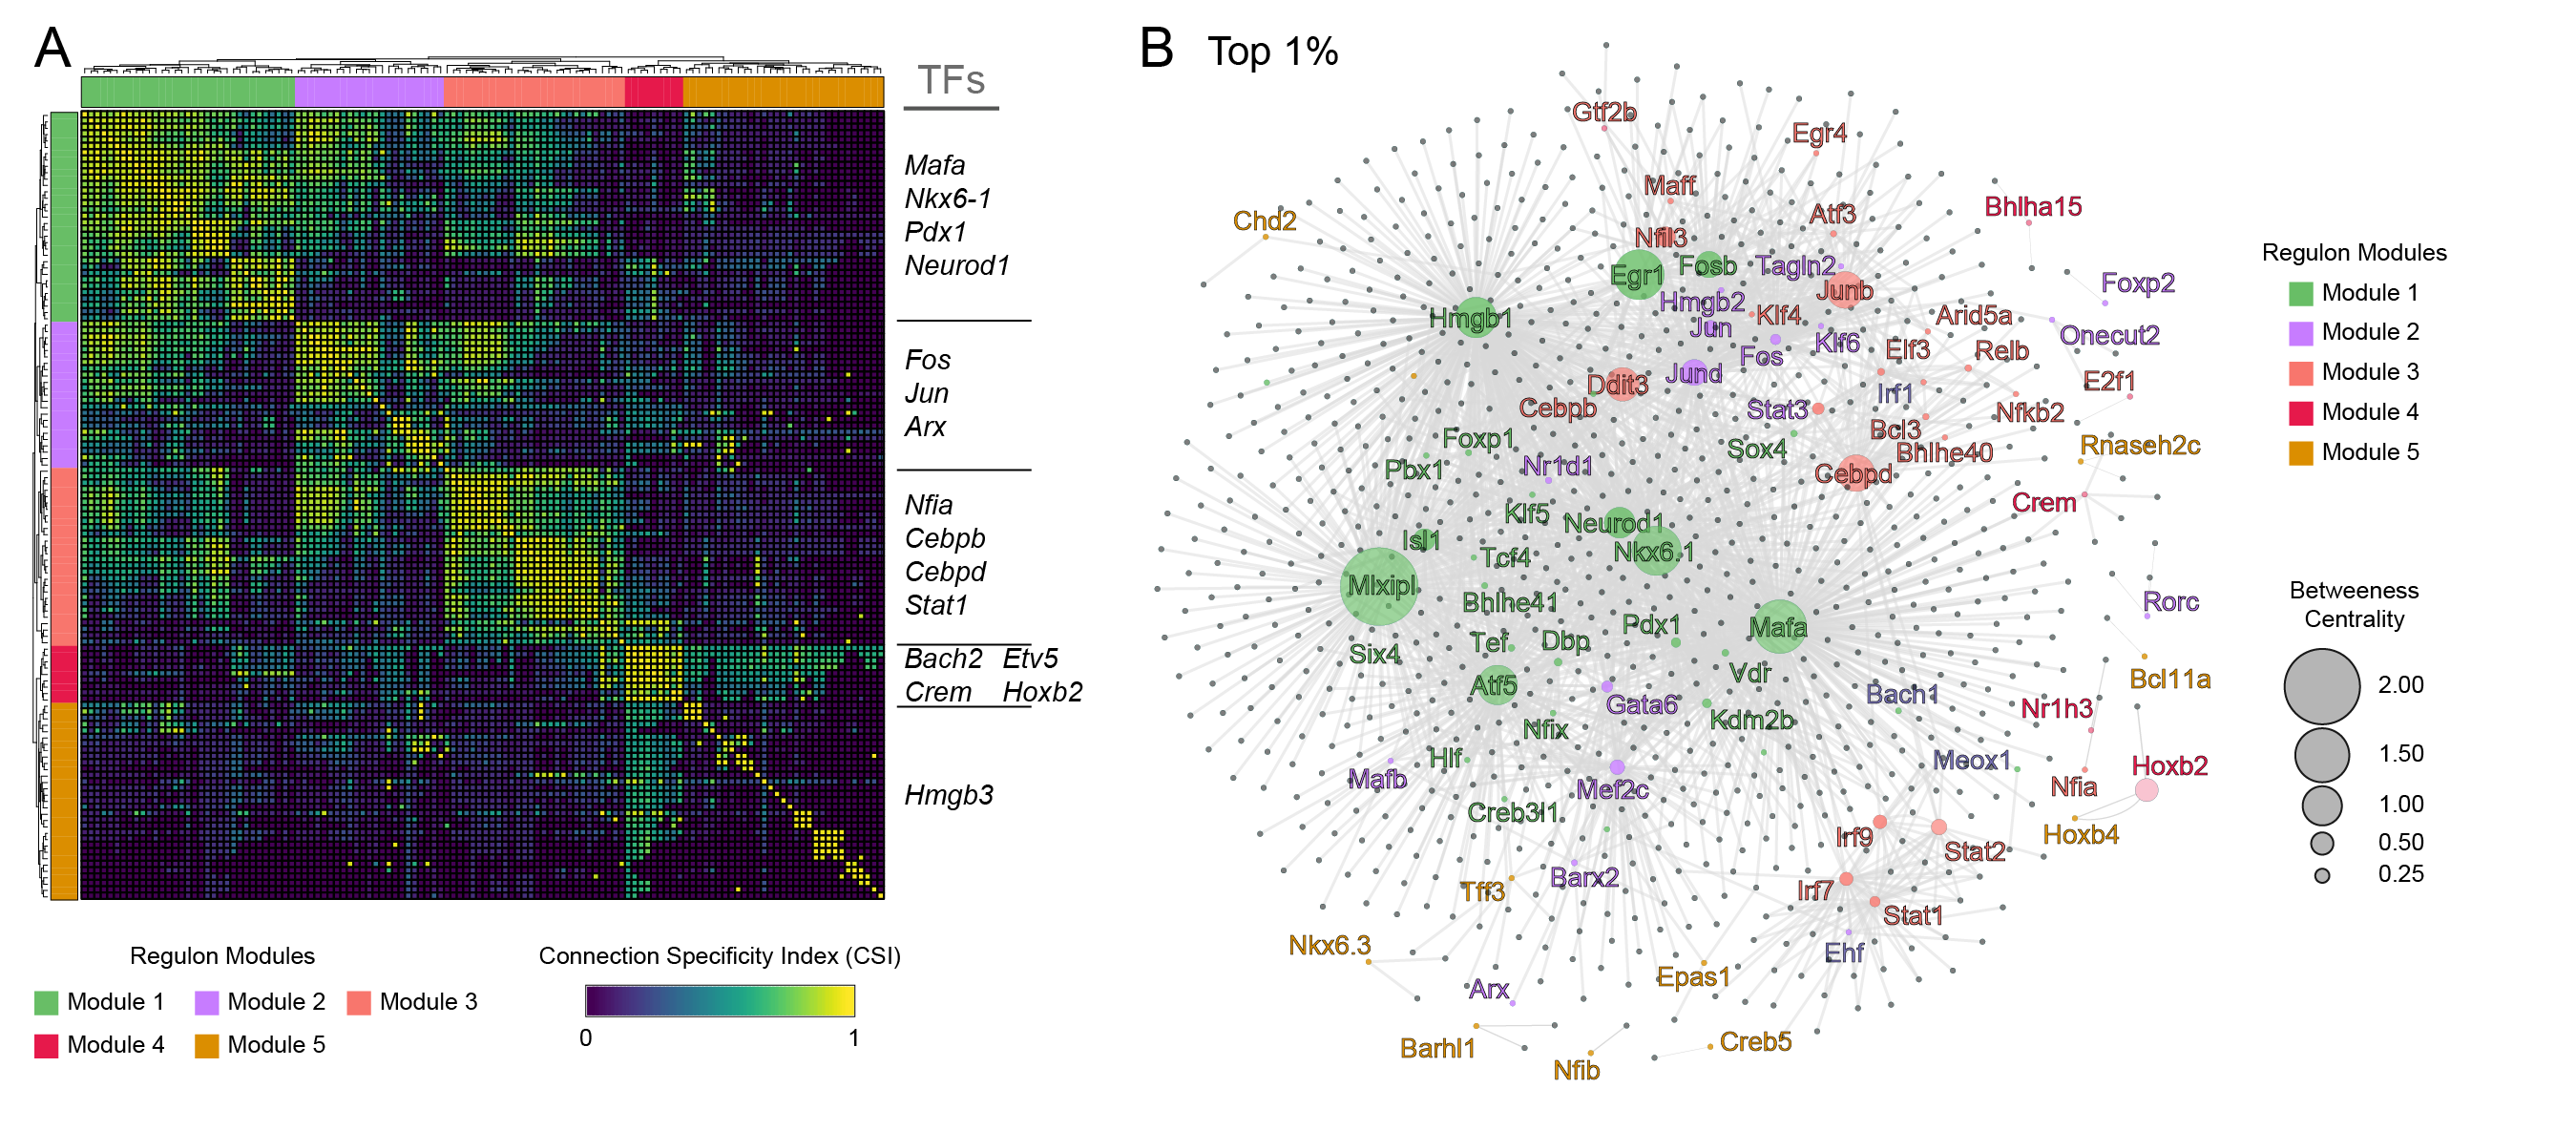
\includegraphics[width=\linewidth]{Chapter5/Fig/F3-10-02.png}
\caption[Identification of β-cell specific GRN and regulon modules]{\textbf{Identification of β-cell specific GRN and regulon modules}\\}
\label{fig:3-10}
\end{figure}

% \begin{figure}[t]
% \centering
% 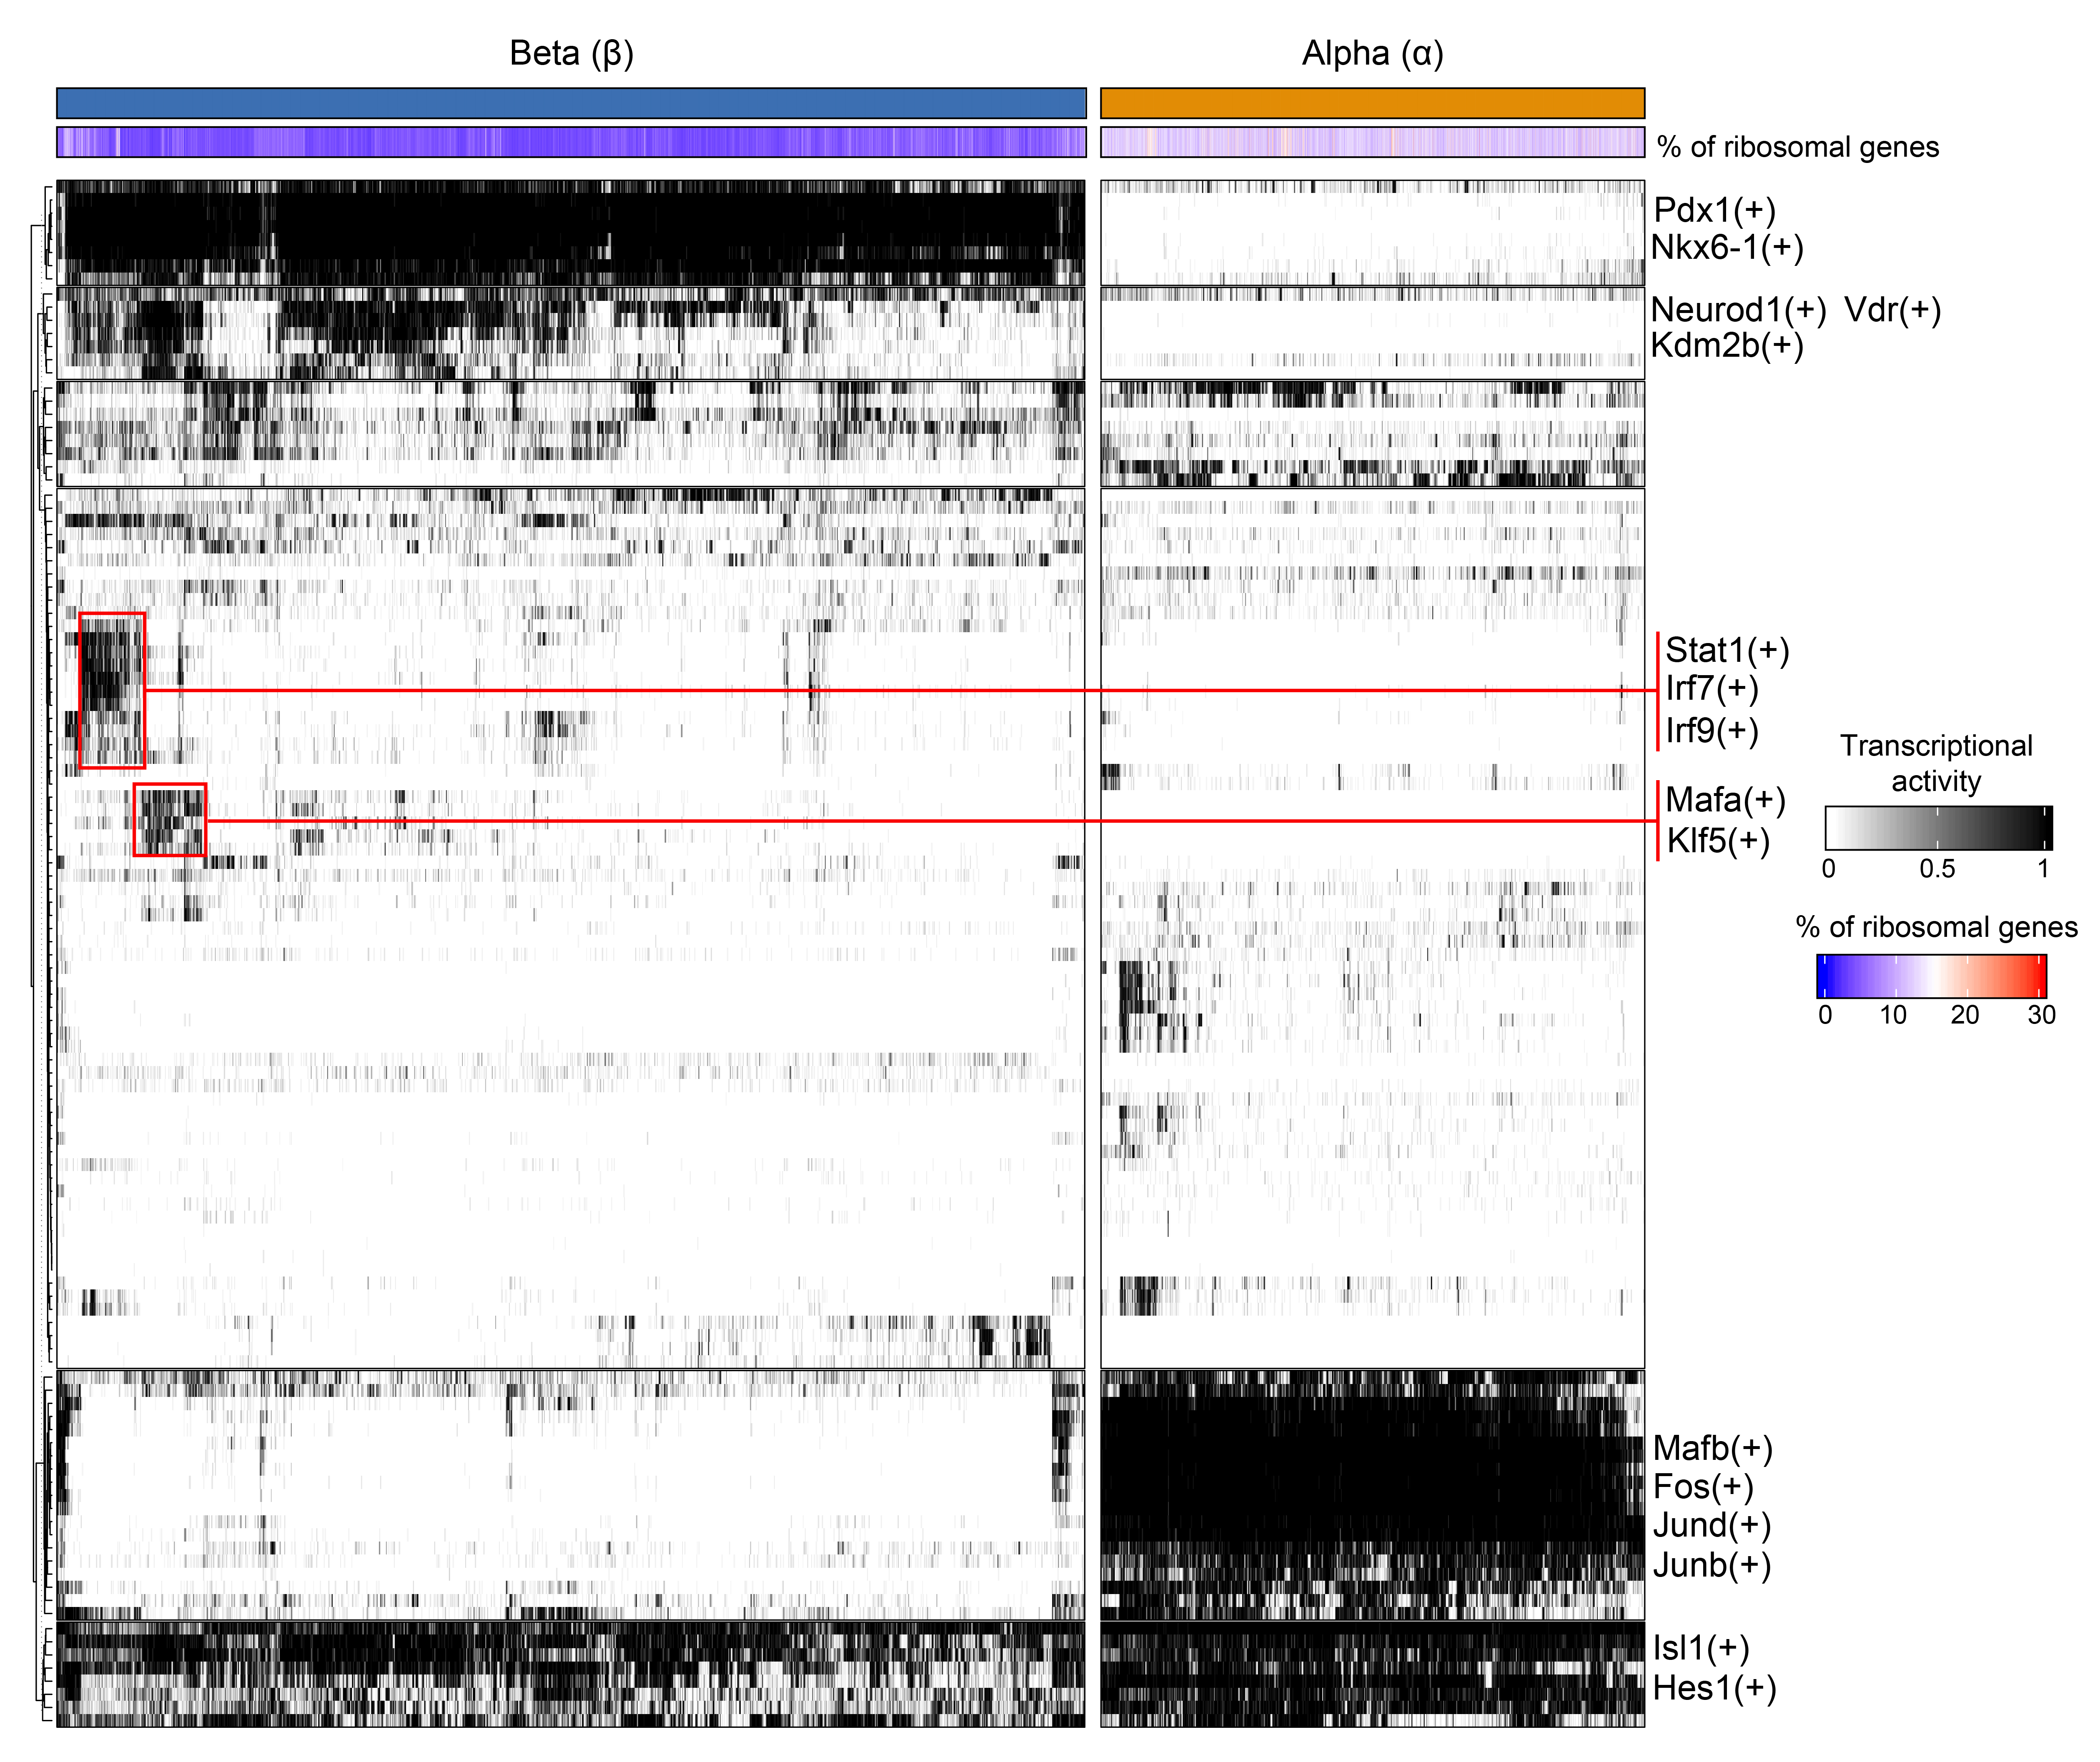
\includegraphics[width=12cm]{Chapter5/Fig/F3-11-01.png}
% \caption[Identification of cell-type specific regulons]{\textbf{Identification of cell-type specific regulons.} Heatmap depicting the binarized \gls{auc} scores, representing the transcriptional activity of regulons across all the cells. Regulons shown in black are considered "ON", while regulons in white are considered "OFF". Several characteristic regulons are highlighted and denoted with `(+)' after the \gls{tf}. The top color bar depicts the cell-type annotation and the bottom color bar depicts the percentage of ribosomal genes in each cell.}
% \label{fig:chp3_scenic_alphabeta}
% \end{figure}

Overall, the observed regulon activity patterns across the various β-cell subsets matched the activity patterns in response to each intervention for all studies. This alignment further supported the robustness of the β-cell subset classification based on functional responses. Critical \gls{tf}-regulons associated with β-cell development and function (\textit{Neurod1, Mafa ,Nkx6-1 ,Pdx1}) clustered together \textbf{(Fig. \ref{})} with the \textit{Neurod1} regulon depicting quantitatively higher activity in the β-1 Normal subset compared to the β-2 Compensating and β-3 Stress-immature subsets \textbf{(Fig. \ref{})}. In addition, the β-1 Normal subset also showed higher activity for \textit{Nfia} regulon \textbf{(Fig. \ref{})}, which is known to regulate endocrine fate induction \textbf{\cite{scavuzzo_pancreatic_2018}} and regulates pancreatic physiology through granule recruitment and docking \textbf{\cite{scavuzzo_nfia_2019}}. We were also able to identify a novel candidate regulator, \textit{Kdm2b}, with regulon activity similar to that of the \textit{Neurod1} regulon \textbf{(Fig. \ref{})}. Examining the target genes of \textit{Kdm2b}, we identified important genes relating to  β-cell function thereby possibly suggesting some important role for this regulon in the context of β-cells. Further, the activity of this regulon was down-regulated in all stress-associated models compared to their corresponding controls \textbf{(Fig. \ref{})}. Therefore, \textit{Kdm2b} might regulate stress responses such as senescence, which has been implicated in both, \gls{t1d} and \gls{t2d}.\\ 

The pySCENIC analysis also revealed that the down-regulation of regulons such as \textit{Vdr, Pknox1, Elk3} and \textit{Meox1} was associated with increasing β-cell workload, resulting in dysfunction and failure. 


%\textit{Kdm2b}, a lysine-specific demethylase, is a critical regulator of definitive hematopoiesis, mediates a gene repressive program that controls hippocampal morphogenesis, represses transcription of ribosomal RNA genes in human cell lines and inhibits the ability of \textit{Cdkn1a}/\textit{p21} to promote senescence in fibroblasts.

%The largest module, \textit{Module 1}, contained TFs associated with β-cell function (\textit{Mafa, Nkx6-1}) and development (\textit{Neurod1, Pdx1}) \textbf{(Fig. \ref{fig:3-10})}. The mean regulon activity of \textit{Mafa} and \textit{Pdx1} was comparable across all subsets \textbf{(Fig. \ref{fig:3-12})}. The activity of \textit{Tcf7l2}, a master regulator of insulin production and processing, and its downstream target \textit{Isl1} were also similar across all subsets. Interestingly, the mean activity of \textit{Neurod1} regulon was (quantitatively) higher for β-1 Normal subset and was down-regulated in β-2 and β-3 subsets. Another interesting TF-regulon with similar activity and expression pattern is \textit{Kdm2b}. \hl{<Stuff about \textit{Kdm2b}>}. Module 1 also included \textit{Atf5}, which has been shown to be an important regulator of ER stress and apoptosis in mouse β-cells \textbf{\cite{ma_atf5_2023}}, and \textit{Hmgb1}, a chromatin protein that can induce autophagy by activating various pathways and has been shown to play an important role in insulin resistance and diabetes \textbf{\cite{yang_relationship_2023}} \textbf{(Fig. \ref{fig:3-12})}. \hl{<Stuff about \textit{Vdr}>}\\

%\textit{Module 2} was characterized by the presence of \textit{Fos} and \textit{Jun} regulons, which are components of the activator protein-1 (AP-1) TF complex, and are involved in stress response and have been implicated in the regulation of β-cell function, particularly under conditions of metabolic stress or diabetes. \textit{Jund}, a member of the \textit{Jun} family, in particular,  has been found to be up-regulated  in response to high concentrations of glucose and free fatty acids, and its depletion can block the increase in oxidative stress and apoptosis in β-cells during glucolipotoxicity \textbf{\cite{good_jund_2019}}. Strikingly, this module also contained the TF \textit{Arx}, which specifies the formation of pancreatic islet α-cell during development. The \textit{Arx} regulon was active in both, the β-3 Stress-immature and the β-5 Dev.-immature subsets. The higher activity of \textit{Arx} in β-3 compared to β-1 or β-2 subsets likely suggests the activation of a dedifferentiation like-program in response to increased workload in hyperglycemic and insulin-resistant models. The forced over-expression of \textit{Arx} within pancreata showed massive reductions in beta and delta cell numbers and increased alpha and PP cell numbers \textbf{\cite{van_der_meulen_role_2015}}. This (trans/de)-differentiation could be mitigated by the activity of \textit{Klf6} regulon, a downstream effector of \textit{Sox9} \textbf{\cite{puri_sox9_2024}} and an immediate early response gene \textbf{\cite{xin_single-cell_2016}}, in β-2 subset, as \textit{Klf6} has been shown to protect β-cells against insulin-resistance induced dedifferentiation. \textit{Klf6} knockout mice displayed stronger β-cell dysfunctions against insulin resistance (WD-feeding) with severe hyperglycemia (S961 treatment) \textbf{\cite{dumayne_klf6_2020}}. \hl{<Stuff about \textit{Taf7,Rorc}>}\\



%\textit{Module-3} contained the TFs \textit{Cebpb} and \textit{Cebpd}, which have anti-apoptotic and anti-inflammatory roles in pancreatic β-cells \textbf{\cite{https://www.ncbi.nlm.nih.gov/pmc/articles/PMC3275575/}}. This module was also comprised of members of the IFN regulatory factor (\textit{Irf1, Irf7, Irf8} and \textit{Irf9}) and the signal transducer and activator of transcription (\textit{Stat1,Stat2} and \textit{Stat3}) families, which have essential roles in regulating Type-1 IFN induction and downstream actions, respectively \textbf{\cite{https://www.ncbi.nlm.nih.gov/pmc/articles/PMC6331453/}}. In particular, \textit{Stat1} is a master regulator of β-cell apoptosis and islet inflammation \textbf{\cite{https://www.ncbi.nlm.nih.gov/pmc/articles/PMC3020778/}}. \hl{\textit{Module 4} contained regulons such as \textit{Bach2, Bhlha15, Crem, E2f1, Etv5, Gtf2b, Hoxb2, Mybl1, Nr1h3} which seemed to be uniformly active across all β-subsets, whereas most of the regulons in \textit{Module 5} had no activity in any of the β-subsets. Of note, \textit{Hmgb3} regulon had higher activity in the β-5 Dev.-Immature subset compared to the rest and the \textit{Pou6f2} regulon had a similar profile in β-3 Stress-Immature and β-5 Dev.-Immature subsets.}\\


\begin{figure}[t]
\centering
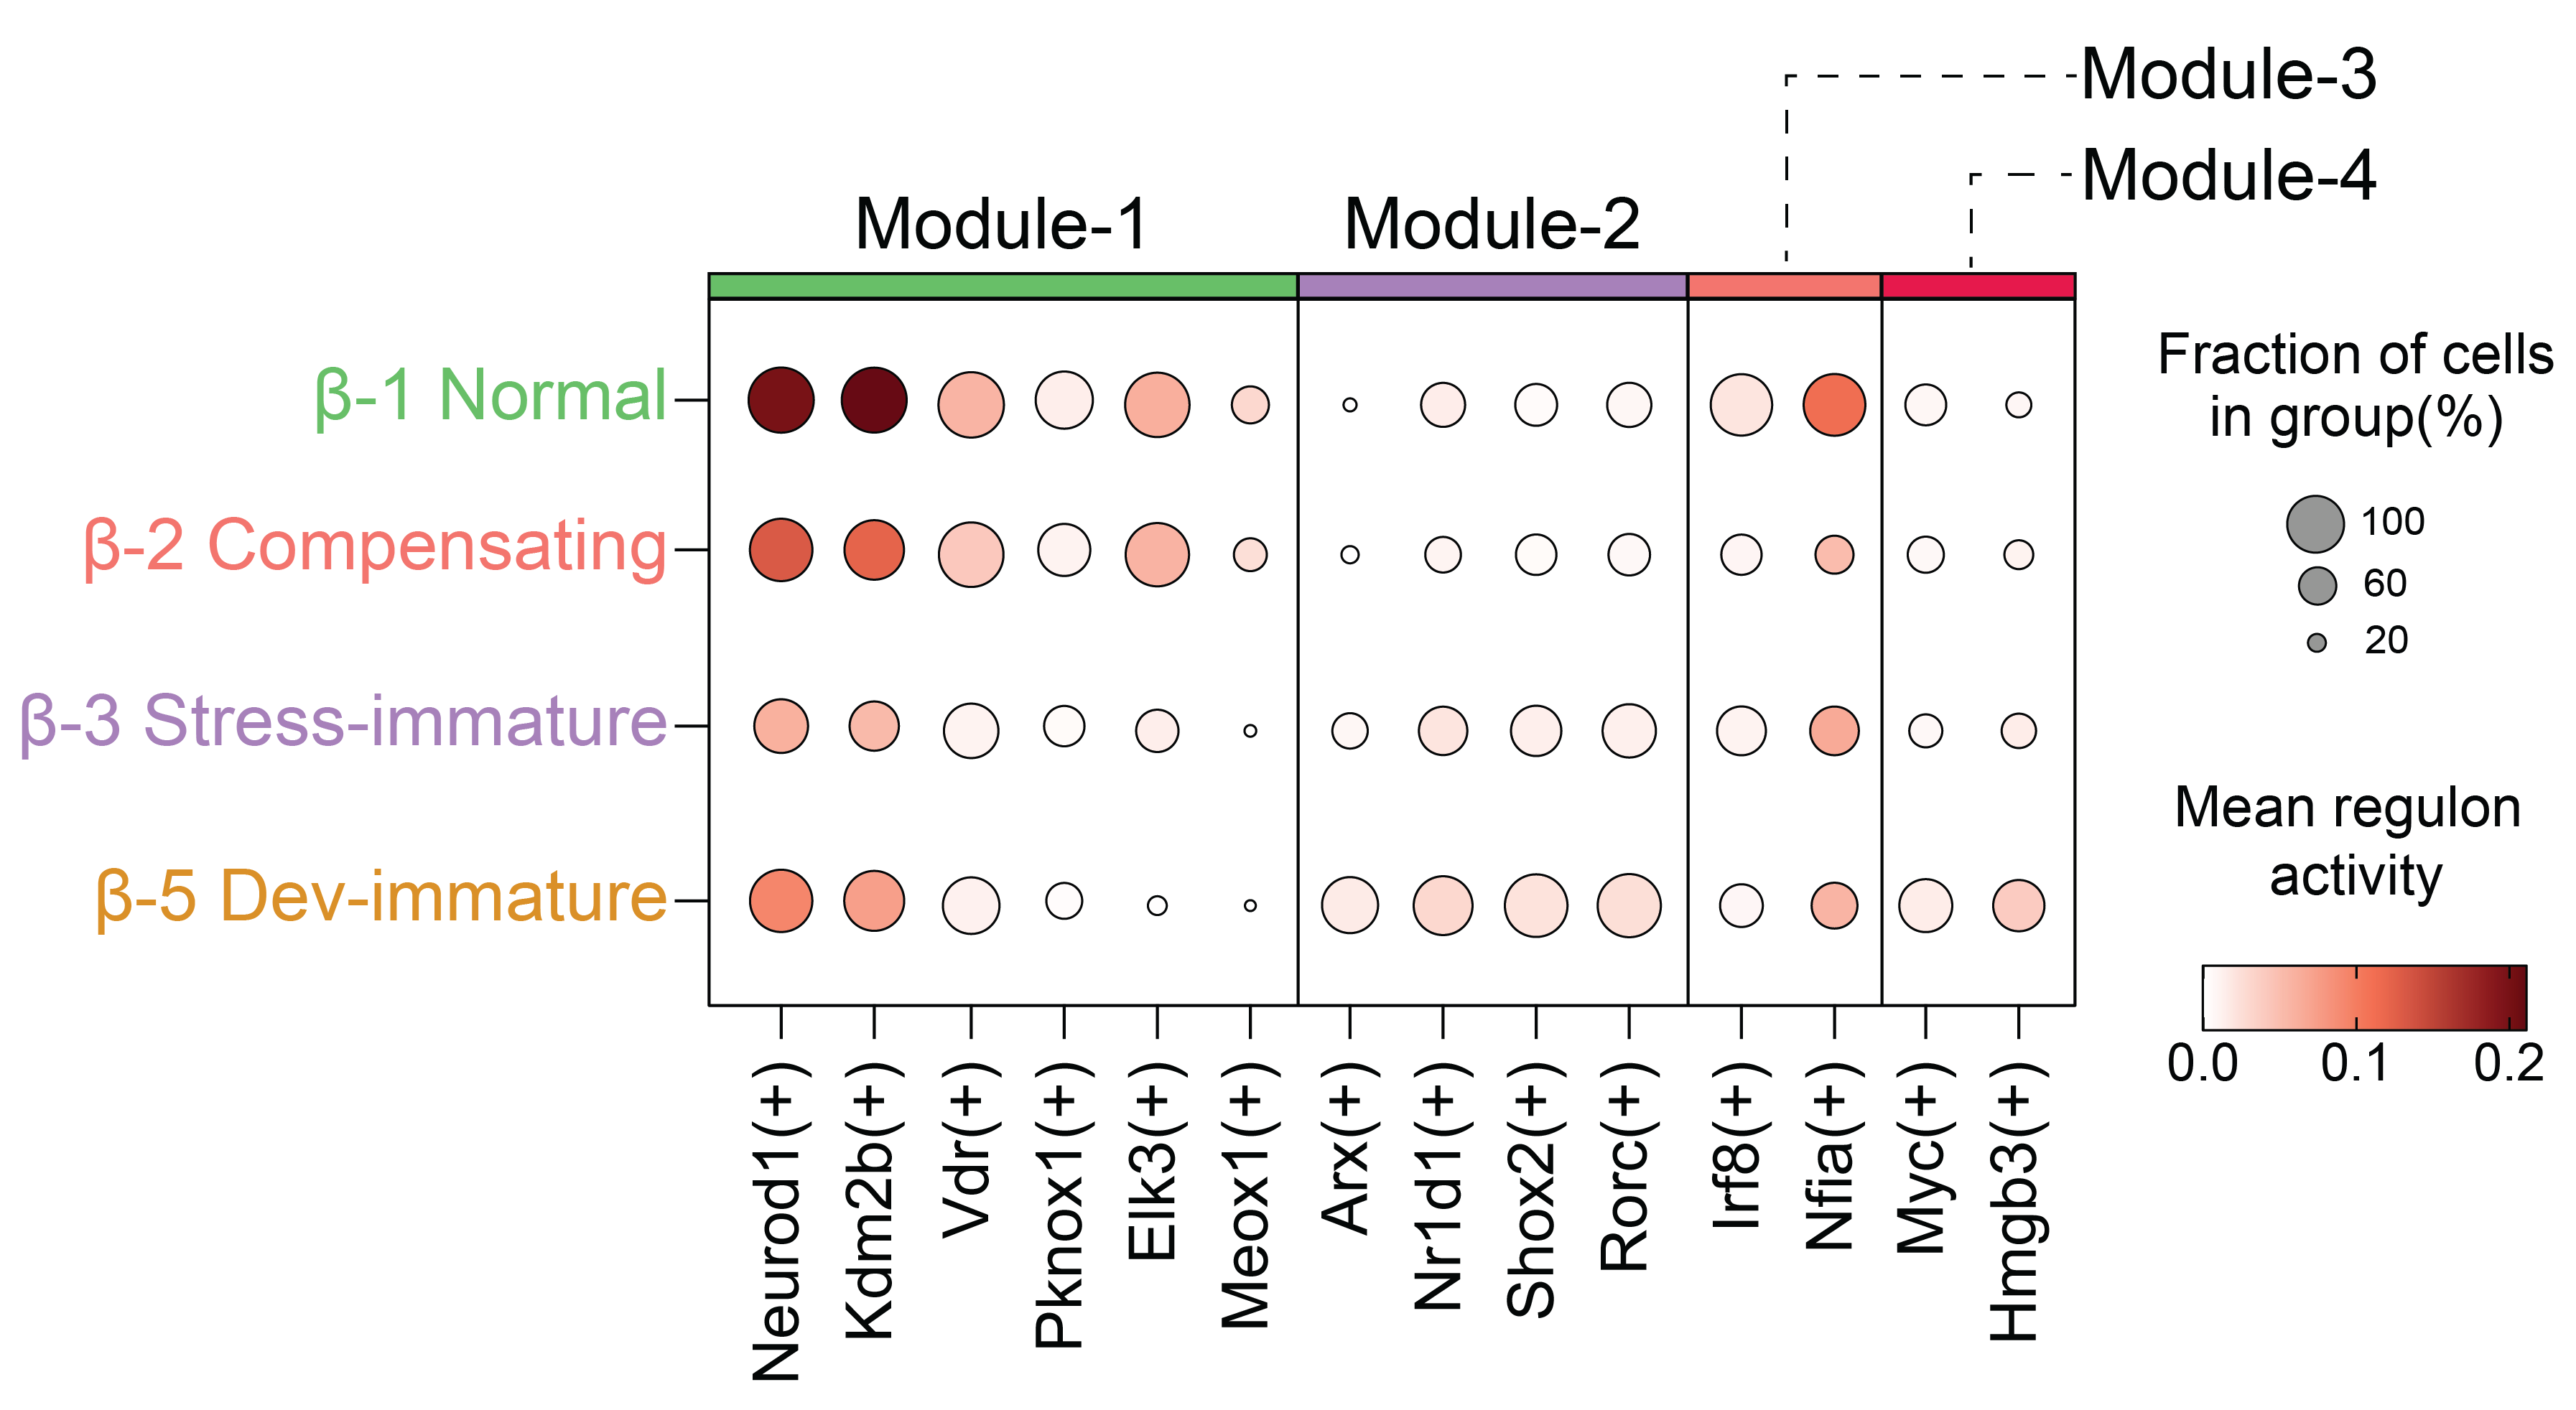
\includegraphics[width=12cm]{Chapter5/Fig/F3-12-v2-01.png}
\caption[Mean regulon activity of all regulons in Module-1 of β-cell GRN]{\textbf{Mean regulon activity of all regulons in Module-1 of β-cell GRN}\\}
\label{fig:3-12-1}
\end{figure}

%\clearpage


% \begin{figure}[H]
% \centering
% \includegraphics[width=\linewidth]{Chapter5/Fig/F3-12-02.png}
% \caption[Mean regulon activity of all regulons in Module-2 of β-cell GRN]{\textbf{Mean regulon activity of all regulons in Module-2 of β-cell GRN}\\}
% \label{fig:3-12-2}
% \end{figure}


%To gain a better understanding about the expression dynamics of \glspl{tf} associated with regulons identified in this analysis, we examined the expression of several candidate \gls{tf} across the Maturity (PC1)-Workload (PC2) axis from \textbf{Section \ref{sec:chp3_betaPCA}}. Consistent with previous analysis, \glspl{tf} associated with β-cell function (\textit{Mafa, Vdr}), \textit{Kdm2b, Atf5} were down-regulated with loss of β-cell maturity. Conversely, the expression of \glspl{tf} such as \textit{Egr1, Hmgb1, Mafb, Mlxipl} and components of the AP-1 complex were correlated with the stress- and  developmentally- immature β-cell subsets. Interestingly, while the expression of key \glspl{tf} like \textit{Neurod1} and \textit{Nkx6-1} in the β-5 Dev-immature subset is expected, they were also up-regulated with the loss of maturity in response to insulin resistance and hyperglycemia. \hl{Along the workload axis, ...}\\\\
\hl{In summary ....}

\clearpage

\section{Transcriptional similarity of mouse models to human \gls{t2d}}
\label{sec:chp3_T2Dgenes}
Rodent models play a crucial role in the study of \gls{t2d}, offering insights into disease pathogenesis, progression and potential therapeutic interventions. These models are invaluable due to their physiological similarities to humans, including the development and progression of \gls{t2d}. The different models vary in how closely they mimic the natural progression of human \gls{t2d} and have specific advantages and limitations \textbf{\cite{kleinert_animal_2018, singh_animal_2024}}. Given the broad range of β-cell workload models included in this study, we wanted to further asses the extent of similarity of transcriptional profiles of these models to human T2D. Extending the assessment made by the \gls{mia} \textbf{\cite{hrovatin_delineating_2023}}, we utilized gene-sets enriched in human \gls{t2d} and scored for these across all non-proliferating β-cells in our analysis. These included gene-sets related to pancreas development, hormone metabolism, ribosome biogenesis, protein or peptide breakdown by proteasome and transport vescile of the constitutive secretory pathways. Further, we also assessed the level of up-regulation of several of the characteristic markers associated with these gene-sets by computing fold changes, in order to obtain a gene-level understanding about the dynamics of β-cell workload in response to hyperglycemia and insulin resistance.    %The scores of these gene-sets across all non-proliferating β-cells were computed (see \hyperref[sec:chp4_methods2]{\textit{Methods}}). %For each of these gene-sets, we first identified the orthologous genes in our mouse dataset and then performed gene-set scoring on a single-cell level.\\

\subsubsection{Endocrine Pancreas Development}
The gene-set `Endocrine pancreas development' was down-regulated in all datasets compared to their respective controls \textbf{(Fig. \ref{fig:chp3_gs_endo} A)}. This was also observed in the \gls{mia} which included \textit{db/db} animals with established hyperglycemia as well as the partial β-cell ablation model (which has been included in this study). However, since this gene-set was enriched among human T2D-up-regulated genes, the unexpected direction of the gene-set change in the mouse T2D models could be attributed to the diversity of the genes. The gene-set includes genes related β-cell maturation as well as β-cell immaturity, which likely affected the scoring. We therefore examined specific genes from this gene-set \textbf{(Fig. \ref{fig:chp3_gs_endo} B)}. The expression of several characteristic β-cell identity and functional genes in this set were mildly down-regulated in all stress models except in case of feeding intervention and S961-treatment. Genes such as \textit{Gipr, Neurod1, Nkx2-2, Nkx6-1} were mildly up-regulated in the fed mice whereas S961-treatment induced the up-regulation of \textit{Foxa2, Insm1, Nkx2-2}  and \textit{Pdpk1}. \hl{Add reasoning}

\begin{figure}[H]
\centering
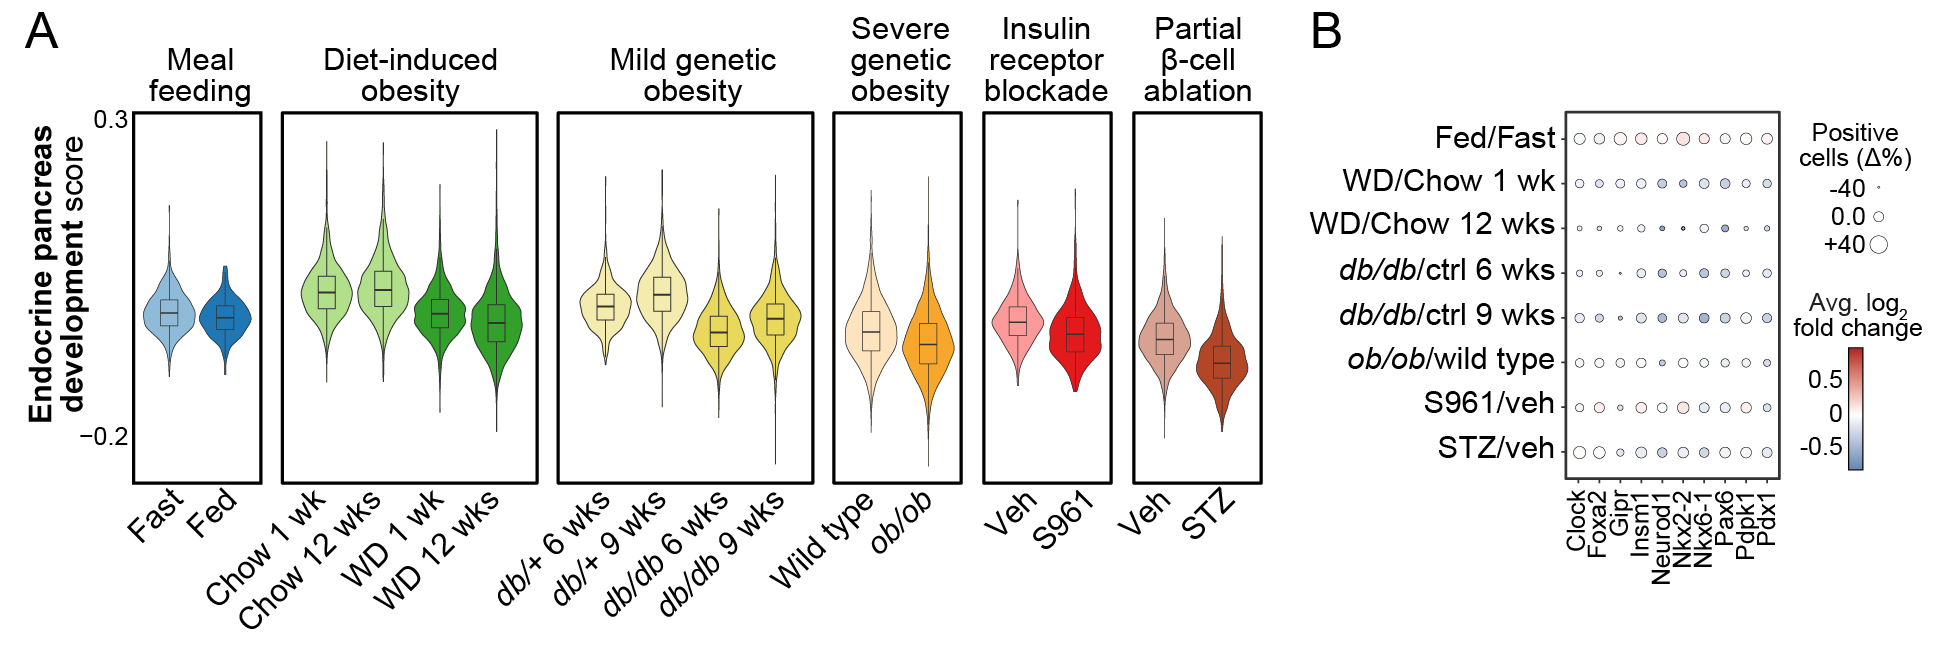
\includegraphics[width=\linewidth]{Chapter5/Fig/F3-13-01.png}
\caption[Scoring of gene-set - \textit{Endocrine pancreas development}]{\textbf{Activity of genes associated with Endocrine pancreas development.} \textbf{(A)} Violin plots depicting the gene-set score for `Endocrine pancreas development' associated genes shown for β-cell workload models and corresponding healthy controls from individual studies. On the overlay boxplots, the middle horizontal line represents the median, the box represents the inter-quartile range and the whiskers represent the minimum and maximum values. The number of cells are indicated in Supplementary Table \ref{tab:3-3}. \textbf{(B)} Differential expression of few of the `Endocrine pancreas development' associated genes across β-cell workload models compared to their respective controls. The color and size of the dots represent the average log fold change of expression and the difference in percentage of cells between the models and their respective controls.}
\label{fig:chp3_gs_endo}
\end{figure}


%\clearpage

\subsubsection{Hormone Metabolism}
\label{subsec:hormone}
Similar to the observations in \gls{mia}, genes related to hormone metabolic processes were strongly up-regulated in all models β-cell workload, except for Meal feeding and Diet-induced obesity models \textbf{(Fig. \ref{fig:chp3_gs_hm} A)}. The strong up-regulation of several characteristic genes in the young \textit{db/db} animals was complementary to the up-regulation observed in older \textit{db/db} models employed in the \gls{mia}. Genes such as \textit{Pam}, phogrin (\textit{Ptprn}), secretogranin 3 (\textit{Scg3}) were up-regulated in both, 6-wks-old and 9-wks-old \textit{db/db} animals, with \textit{Ptprn, Scg3} depicting stronger up-regulation at the 9-wks time-point \textbf{(Fig. \ref{fig:chp3_gs_hm} B)}. \textit{Ptprn}, which is primarily localized on INS-secretory granules in β-cells, plays a crucial role in the overall regulation of glucose-stimulated insulin signalling in β-cells \textbf{\cite{torii_pseudophosphatase_2018}}. \textit{Scg3} plays a crucial role in regulating biogenesis of secretory granules that contain hormones in endocrine cells and assits in insulin processing, thus affecting glucose homeostasis \textbf{\cite{lin_serum_2019}}. These genes were also up-regulated in the hyperglycemia models of severe genetic obesity, insulin receptor blockade and the partial β-cell ablation. Hyperglycemia induced by chemial treatments (S961 and \gls{stz}) also resulted in stronger up-regulation of additional genes such as \textit{Cpe, Syp, Syt5} and \textit{Tmed10} \textbf{(Fig. \ref{fig:chp3_gs_hm} B)}.


\begin{figure}[t]
\centering
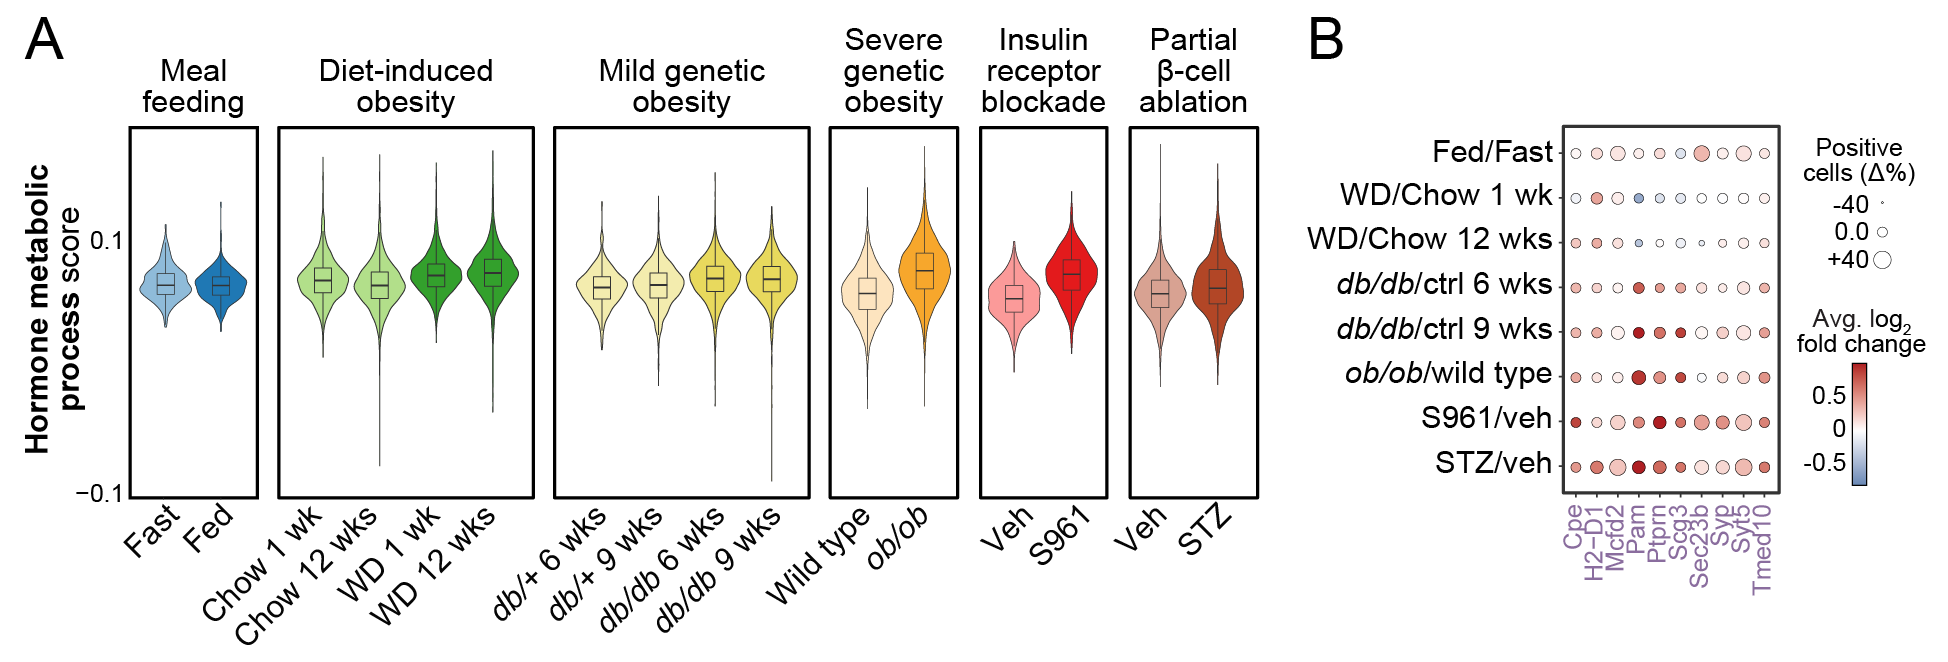
\includegraphics[width=\linewidth]{Chapter5/Fig/F3-13-02.png}
\caption[Scoring of gene-set - \textit{Hormone Metabolic process}]{\textbf{Activity of genes associated with Hormone metabolic process.} \textbf{(A)} Violin plots depicting the gene-set score for `Hormone metabolic process' associated genes shown for β-cell workload models and corresponding healthy controls from individual studies. On the overlay boxplots, the middle horizontal line represents the median, the box represents the inter-quartile range and the whiskers represent the minimum and maximum values. The number of cells are indicated in Supplementary Table \ref{tab:3-3}. \textbf{(B)} Differential expression of few of the `Hormone metabolic process' associated genes across β-cell workload models compared to their respective controls. The color and size of the dots represent the average log fold change of expression and the difference in percentage of cells between the models and their respective controls.}
\label{fig:chp3_gs_hm}
\end{figure}


\subsubsection{Ribosome Biogenesis}
Ribosomes are cellular factories that make proteins. Following a similar profile to `Hormone Metabolism', the feeding intervention and WD-induced obesity did not result in a higher activity for genes related to ribosome biogenesis \textbf{(Fig. \ref{fig:chp3_gs_rb} A)}. Several genes were down-regulated in response to these two mild hyperglycemic models \textbf{(Fig. \ref{fig:chp3_gs_rb} B)}. This echoes a similar observation of reduced expression of several ribosome biogenesis genes in a \gls{hfd} model. \textbf{\cite{hatanaka_chronic_2017}}. Conversely, this gene-set was up-regulated in both models of genetic obesity (\textit{db/db} and \textit{ob/ob}) and following S961- and \gls{stz}-treatment \textbf{(Fig. \ref{fig:chp3_gs_rb} A)}. A significant increase in the expression of ribosome-related molecules has been demonstarted in islets isolated from \textit{db/db} mice \textbf{\cite{asahara_increased_2009}}. The strong up-regulation of ribosomal markers in the \textit{ob/ob} mice and following  S961-treatment could be attributed as an response to the  hyperglycemic 
\begin{figure}[H]
\centering
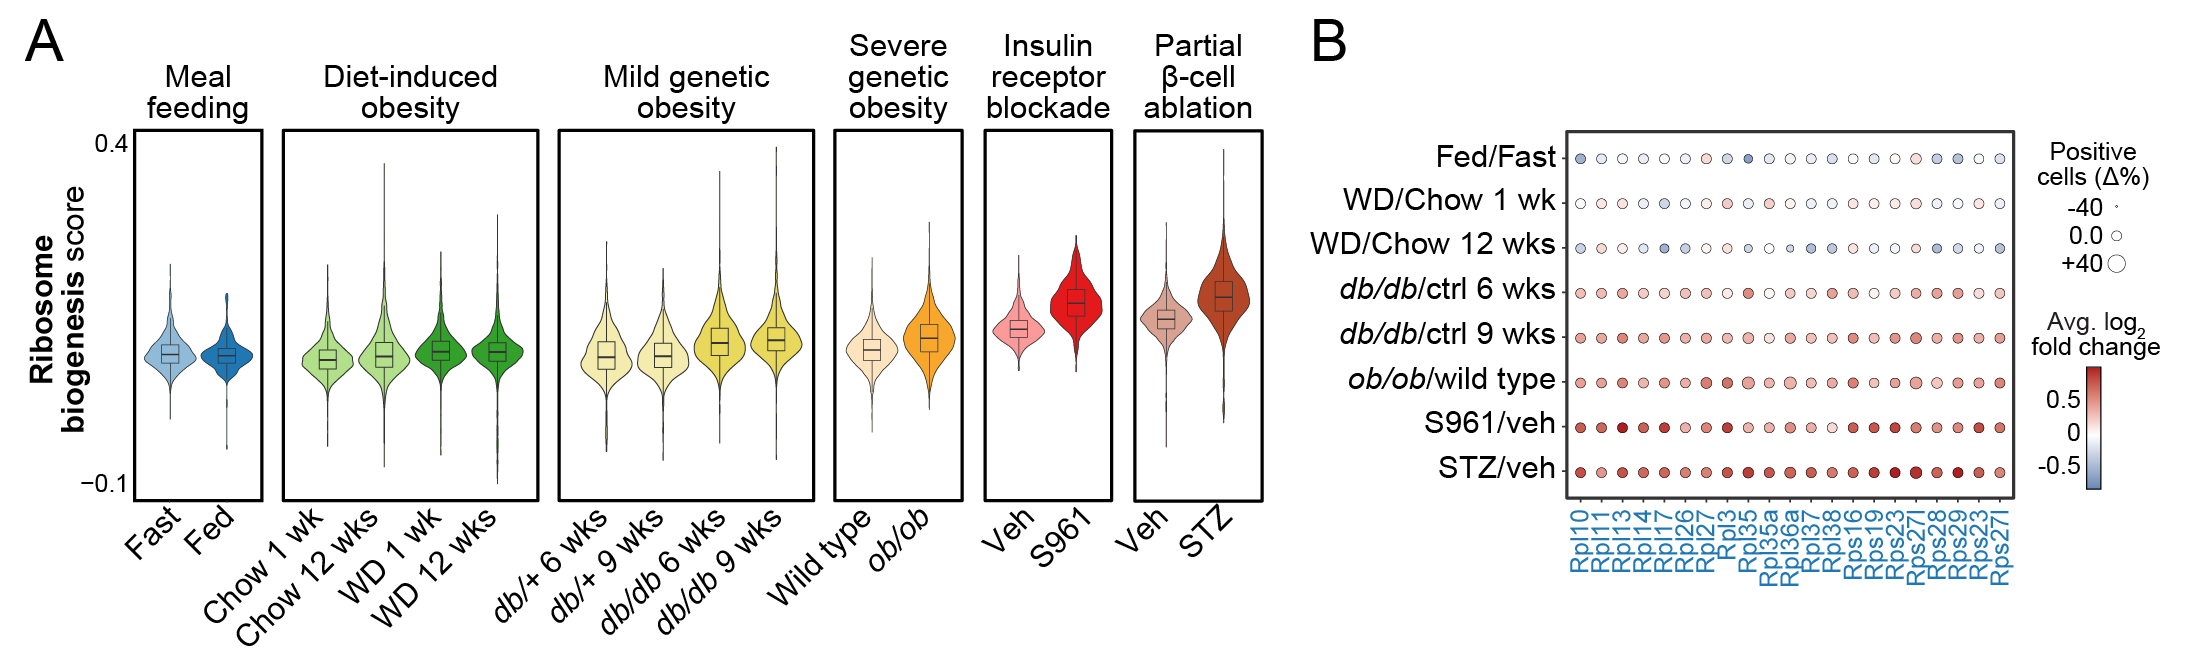
\includegraphics[width=\linewidth]{Chapter5/Fig/F3-13-03.png}
\caption[Scoring of gene-set - \textit{Ribosome Biogenesis}]{\textbf{Activity of genes associated with Ribosome biogenesis.} \textbf{(A)} Violin plots depicting the gene-set score for `Ribosome biogenesis' associated genes shown for β-cell workload models and corresponding healthy controls from individual studies. On the overlay boxplots, the middle horizontal line represents the median, the box represents the inter-quartile range and the whiskers represent the minimum and maximum values. The number of cells are indicated in Supplementary Table \ref{tab:3-3}. \textbf{(B)} Differential expression of few of the `Ribosome biogenesis' associated genes across β-cell workload models compared to their respective controls. The color and size of the dots represent the average log fold change of expression and the difference in percentage of cells between the models and their respective controls.}
\label{fig:chp3_gs_rb}
\end{figure}

environment leading to  compensatory, increased insulin production and this effect is amplified in case of \gls{stz}-treatment, where the surviving population of β-cells following ablation are unable to prevent hyperglycemia \textbf{(Fig. \ref{fig:chp3_gs_rb} B)}. The up-regulation of the ribosomal markers in the three hyperglycemic models was also consistent with the expression of ribosomal protein genes correlating with loss of β-cell maturity along the the Maturity (PC1) axis \textbf{(Fig. \ref{fig:chp3_pc1} B)}.

\subsubsection{Proteasomal Catabolic process}
The gene-set `Proteasomal Catabolic process' was up-regulated in all models of increasing β-cell workload \textbf{(Fig. \ref{fig:chp3_gs_pcp} A)}. The genes comprising this gene-set were canonical unfolded protein response (UPR) and endoplasmic reticulum (ER)-associated protein degradation (ERAD) markers. The UPR is a critical adaptive response to ER stress, restoring cell homeostasis and contributing to loss of β-cell mass in T2D \textbf{\cite{oppenlander_vertical_2021,fonseca_endoplasmic_2011,bilekova_pharmacological_2021}}. UPR genes such as \textit{Hspa5, Edem2, Derl3} and \textit{Herpud1} were found to be up-regulated on the mRNA level in response to various models of increasing β-cell workload \textbf{(Fig. \ref{fig:chp3_gs_pcp} B)}. The ERAD pathway serves to mitigate ER stress and has been attributed an indispensable role in the maintenance of β-cell identity and function \textbf{\cite{oppenlander_vertical_2021,hu_endoplasmic_2019,shrestha_sel1l-hrd1_2020}}. The expression of ERAD genes such as \textit{Derl3, Dnajb9, Edem1/2, Herpud1, Hspa5, Hsp90b1, Sec61b, Selenos} were also up-regulated in all studies \textbf{(Fig. \ref{fig:chp3_gs_pcp} B)}. Therefore, increases in β-cell workload enhances adaptive-response mechanisms to ER stress in β-cells in response to \hl{...}

\begin{figure}[H]
\centering
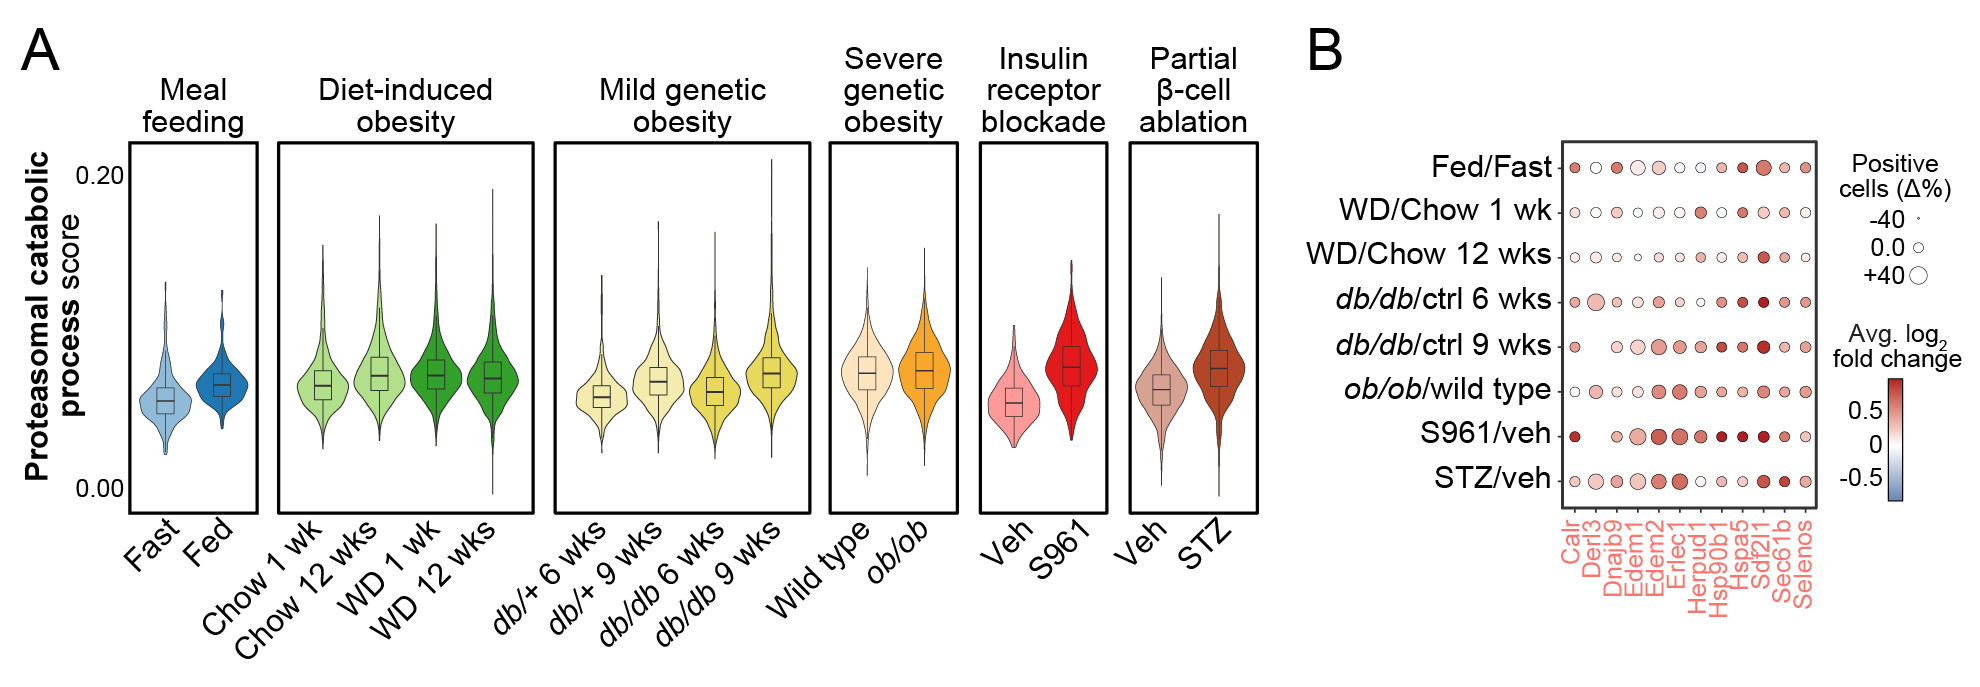
\includegraphics[width=\linewidth]{Chapter5/Fig/F3-13-04.png}
\caption[Scoring of gene-set - \textit{Proteasomal Catabolic process}]{\textbf{Activity of genes associated with Proteasomal catabolic process.} \textbf{(A)} Violin plots depicting the gene-set score for `Proteasomal catabolic process' associated genes shown for β-cell workload models and corresponding healthy controls from individual studies. On the overlay boxplots, the middle horizontal line represents the median, the box represents the inter-quartile range and the whiskers represent the minimum and maximum values. The number of cells are indicated in Supplementary Table \ref{tab:3-3}. \textbf{(B)} Differential expression of few of the `Proteasomal catabolic process' associated genes across β-cell workload models compared to their respective controls. The color and size of the dots represent the average log fold change of expression and the difference in percentage of cells between the models and their respective controls.}
\label{fig:chp3_gs_pcp}
\end{figure}


\subsubsection{Transport Vesicle}
Diet models such as the feeding intervention and diet-induced obesity exhibited opposite patterns for the ‘Transport Vesicle’ gene-set \textbf{(Fig. \ref{fig:chp3_gs_tv} A)}.  Feeding intervention resulted in minor up-regulation of the gene-set while exemplary genes did not show a high magnitude of fold-change \textbf{(Fig. \ref{fig:chp3_gs_tv} B)} whereas diet-induced obesity after 1 or 12-weeks of feeding down-regulated the overall gene-set, although some of the genes were up-regulated by a higher magnitude than feeding intervention \textbf{(Fig. \ref{fig:chp3_gs_tv} B)}. This could be explained by an acute increase in transport vesicle dynamics upon feeding compared to chronic effects of obesity induced by a \gls{hfhsd}, and therefore the down-regulation of these processes. Genetic pre-disposition to diabetes via the \textit{db/db} and \textit{ob/ob} models also exhibited an up-regulation of the vesicle gene-set, although the magnitude in the  \textit{ob/ob} model was lower \textbf{(Fig. \ref{fig:chp3_gs_tv} A)}. The treatment-induced hyperglycemic models such as S961-treatment and \gls{stz}-treatment were strongly associated with changes in transport vesicle (\textit{Atp1a1, Stub1}) \textbf{(Fig. \ref{fig:chp3_gs_tv} B)}. This strong up-regulation could be a result of activation of responses to cellular stress as way for β-cells to maintain function by increasing the expression of genes.\\

\begin{figure}[H]
\centering
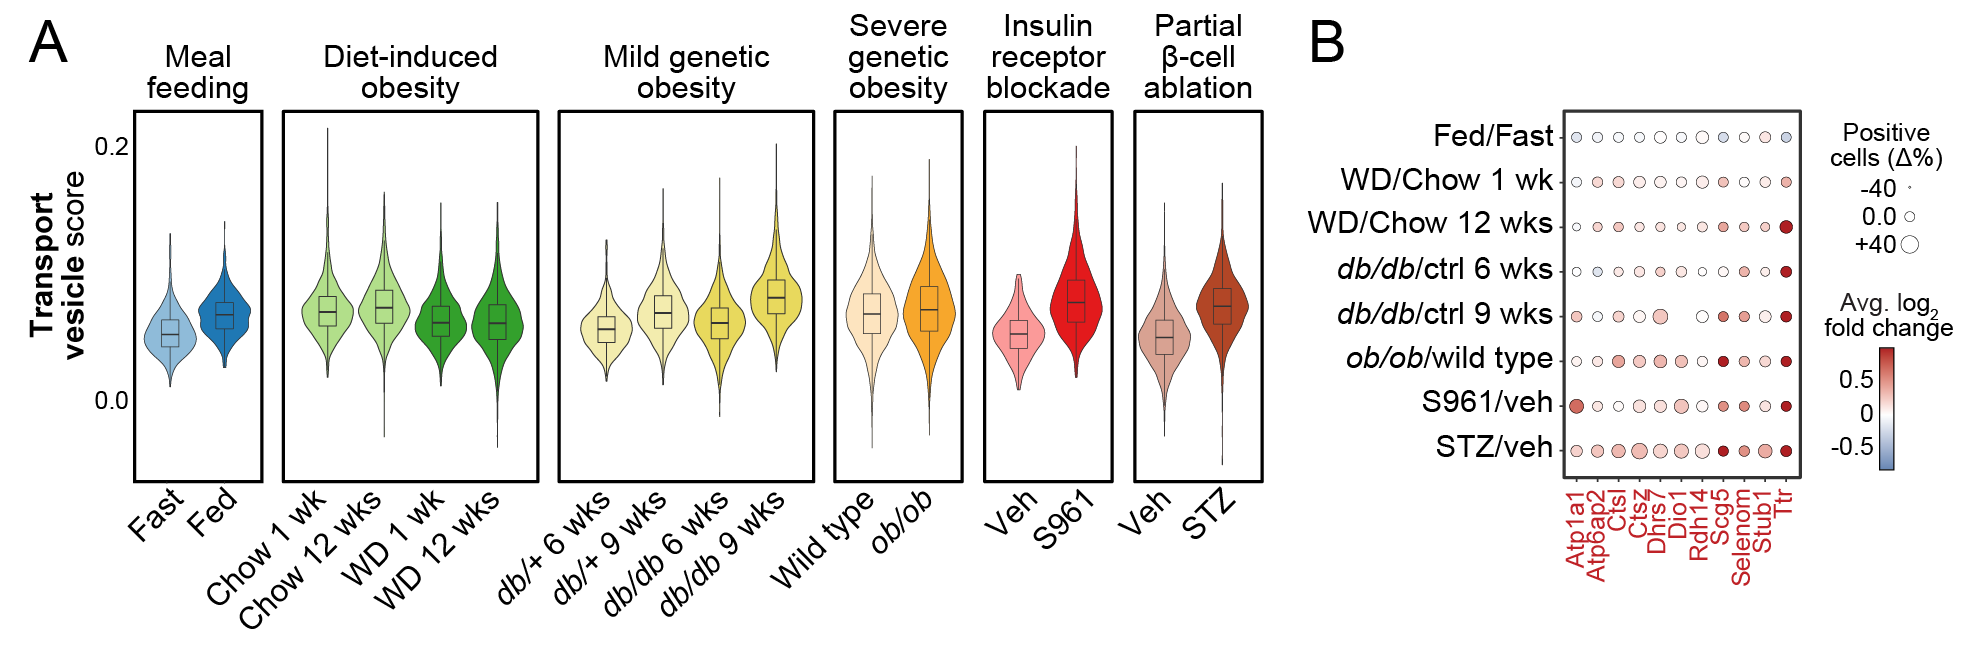
\includegraphics[width=\linewidth]{Chapter5/Fig/F3-13-05.png}
\caption[Scoring of gene-set - \textit{Transport Vesicle}]{\textbf{Activity of genes associated with Transport vesicle across studies.} \textbf{(A)} Violin plots depicting the gene-set score for `Transport vesicle' associated genes shown for β-cell workload models and corresponding healthy controls from individual studies. On the overlay boxplots, the middle horizontal line represents the median, the box represents the inter-quartile range and the whiskers represent the minimum and maximum values. The number of cells are indicated in Supplementary Table \ref{tab:3-3}. \textbf{(B)} Differential expression of few of the `Transport-vesicle' associated genes across β-cell workload models compared to their respective controls. The color and size of the dots represent the average log fold change of expression and the difference in percentage of cells between the models and their respective controls.}
\label{fig:chp3_gs_tv}
\end{figure}


In summary, β-cell compensatory responses to heightened demands of increased workload resulted in overall down-regulation of markers related to β-cell identity and function, and induced pathways related to ER and metabolic stress,  and up-regulated cellular machinery related to ribosomal biogenesis and  vesicle trafficking. Further, this analysis served as extension to the \gls{mia} by recapitulating the findings of similarity between human T2D and mouse models of β-cell dysfunction in the context of mild and severe hyperglycemia. %diet and feeding induced stress, severe genetic obesity and insulin receptor blockade by S961-treatment. 

\clearpage

\section{ \( \mathbf{\upbeta} \)-cell subtype shifts in response to unrestrained insulin\\secretion during obesity via annotation transfer}
\label{sec:chp3_validation}

%A major advantage of single-cell atlases is the ability to learn and transfer the findings from a reference study onto an external query dataset. This is particularly useful in cases of cell-type or state transfer between two or more studies as well as for comprehensive comparisons across several studies and/or conditions. Reciprocally, the atlases can benefit from transfer learning as it enhances the utility and applicability of these resources. The mapping of wide-variety of single-cell datasets exploring various aspects of development, health and disease onto references ultimately extends the scope of the atlases, thereby allowing for further refinement of cell-type annotation, improved data integration and robustness to data variability and facilitating discovery of novel biological insights.

The capacity to learn and apply the results from a reference study onto an external query dataset is a significant benefit of single-cell atlases \textbf{\cite{lotfollahi_mapping_2021,lotfollahi_biologically_2023,ye_mapping_2024}}. This is especially helpful for thorough comparisons across multiple studies and/or conditions, as well as for cell-type or state transfer between two or more studies. Reciprocally, the atlases can benefit from transfer learning as it enhances the utility and applicability of these resources. The mapping of wide-variety of single-cell datasets exploring various aspects of development, health and disease onto references ultimately extends the scope of the atlases, thereby allowing for further refinement of cell-type annotation, improved data integration and robustness to data variability and facilitating discovery of novel biological insights.\\

To demonstrate the usefulness of the integrated β-cell transcriptome generated in this analysis, we mapped an external mouse dataset onto this reference. This additional study included an in-house generated dataset of islets from lean and obese, insulin resistant \textit{db/db} mice, with β-cell specific knockout of lysine-specific histone demethylase 1 (\textit{Lsd1}), which restrains the adaptive insulin secretion of β-cells in response to feeding \textbf{\cite{wortham_nutrient_2023}}. The dataset was generated using the 10x scRNA-seq workflow and the raw data was re-processed using a pipeline similar to that used for sample processing and quality control in the integrated atlas. This ensured that technical batch effects didn't influence the subsequent mapping steps. The dataset was projected onto the integrated subset in order to transfer annotations from the reference to the query.

\subsubsection{\large Regulation of adaptive insulin secretion by epigeonome}

In a recent study, Wortham \textit{et al.} elucidated the nuanced regulation of β cell functional adaptation by the epigenome whereby nutrient availability modulates β cell responses through histone hyperacetylation and transcription. Central to this regulation is chromatin modifying lysine-specific histone demethylase 1 (\textit{Lsd1}) that acts as a dynamic regulator of chromatin accessibility in response to acute changes in nutrient state during feeding and fasting cycles. Interestingly, in an insulin-resistant model of chronic β-cell adaptation (\textit{db/db}), the analysis also found overlap with genes up-regulated in acute β cell response to feeding along with hyperacetylation at many of the feeding-induced sites. Additionally, \textit{Lsd1}-bound active chromatin was also enriched for T2D-associated risk variants, suggesting that T2D risk variants can influence the activity of the \textit{Lsd1}-regulated network. Thus, these findings support a model whereby the β-cell adaptation of insulin secretory response is regulated at the level of the epigenome, with influences from environmental nutrient signals and genetic variation \textbf{\cite{wortham_nutrient_2023,aamodt_peeling_2023}}.

%unveiled the islet epigenome as a pivotal regulatory layer in the β-cell functional adaptation to changes in insulin demand. Through integrated studies of β cell physiology, epigenomics, and transcriptomics \\

\subsubsection{\large Study design}

%To further understand why β-cells fail in \textit{Lsd1} knockout obese \textit{db/db} mice, 
To dissect the role of \textit{Lsd1} in β-cell compensatory mechanisms during insulin resistance, scRNA-seq was performed on islets prior to and after the onset of glucose intolerance. The homozygous (\textit{db/db}) obese animals and their corresponding heterozygous (\textit{db/+}) lean mice were crossed with \textit{Lsd1\textsuperscript{fl/fl}} mice, in order to conditionally knockout \textit{Lsd1}, specifically in β-cells \textbf{(Fig. \ref{fig:chp3_valid_study_design})}. 

% This resulted in the following four experimental cohorts \textbf{(Fig. \ref{fig:chp3_valid_study_design})}:
% \begin{itemize}
%     \item Control (\textit{db/+ Lsd1\textsuperscript{fl/+β}})
%     \item Lean mice with \textit{Lsd1} knockout (\textit{db/+ Lsd1\textsuperscript{$\Delta$β}})
%     \item Obese mice with \textit{Lsd1} intact (\textit{db/db Lsd1\textsuperscript{fl/+β}}) and
%     \item Obese mice with \textit{Lsd1} knockout (\textit{db/db Lsd1\textsuperscript{$\Delta$β}})
% \end{itemize}

\begin{figure}[H]
    \centering
    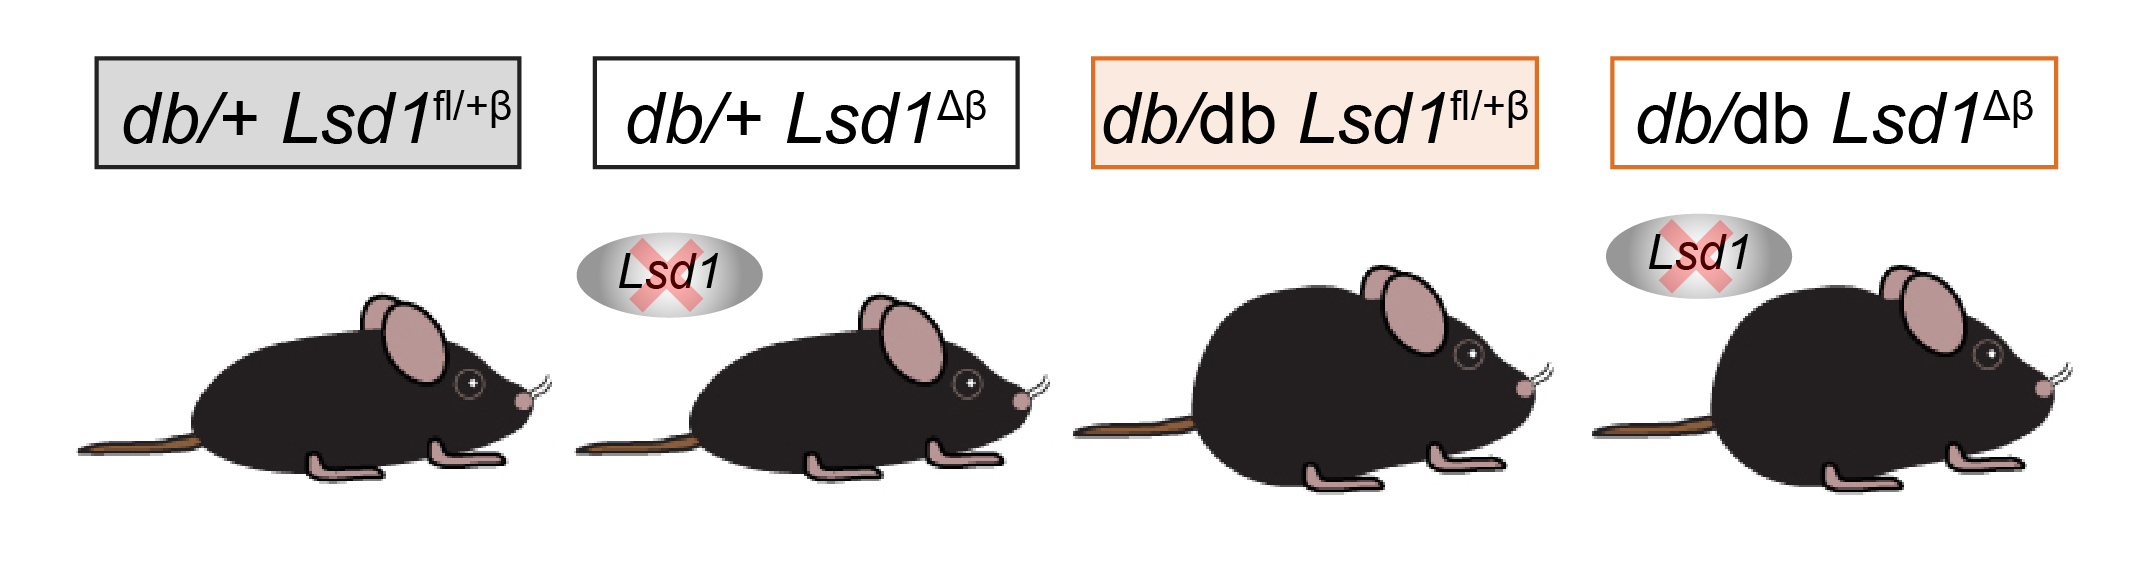
\includegraphics[width=\linewidth]{Chapter5/Fig/F3-17-02.png}
    \caption[Study design of the query dataset]{\textbf{Illustration of the experimental groups in the query dataset.} Islets from lean (\textit{db/+}) and obese (\textit{db/db}) mice with or without intact \textit{Lsd1} in β-cells were isolated and dissociated single cells further processed with the 10x Genomics Chroium technology workflow.}
    \label{fig:chp3_valid_study_design}
\end{figure}


\subsubsection{\large Scoring of gene modules identified across groups from pseudobulk β-cells}

To identify functional processes that are characteristic of the β-cells obtained from the islets of lean and obese mice with or without \textit{Lsd1} knocked-out, we performed gene-set scoring of the modules identified from the hierarchical clustering analysis of pseudo-bulk β-cells across all samples \textbf{(Fig. \ref{fig:chp3_valid_study_genescores})} (\textit{see} Section \ref{sec:chp3_pseudobulk}). As expected, the `Workload-repressed' module was up-regulated in lean mice with \textit{Lsd1} intact \textbf{(Fig. \ref{fig:chp3_valid_study_genescores} A)}. This module consisted of developmental-identity and functional-identity genes. This was also observed in case of the older 9-wks-old animals, wherein the module was further up-regulated compared to the younger 6 wks-old mice. Further, the activity of this module progressively declined in lean mice when \textit{Lsd1} was deleted, followed by obese animals with \textit{Lsd1} intact and \textit{Lsd1} deletion, in which the genes were least active \textbf{(Fig. \ref{fig:chp3_valid_study_genescores} A)}. Interestingly, the 9-wks-old obese mice with \textit{Lsd1} deleted strongly associated with this module in-comparison to their 6-wks-old counterparts. This could likely be due to the additive nature of \textit{db/db} and \textit{Lsd1} effects, which work to enhance insulin secretion, resulting in up-regulation of secretion machinery, but at the cost of later defects.\\\\
The `Workload-activated' and `Decompensation' modules associated in an opposite manner to that of `Workload-repressed' module \textbf{(Fig. \ref{fig:chp3_valid_study_genescores} B,C)}. The obese \textit{db/db} mice with \textit{Lsd1} deletion showed a higher up-regulation of the genes in these modules, with the 9-wks-old animals depicting a stronger trend than the 6-wks-old mice \textbf{(Fig. \ref{fig:chp3_valid_study_genescores} B,C)}. The β-cells in the obese 9-wks-old mice are likely decompensated against the hyperglycemic environment in addition to up-regulation of insulin secretion due to \textit{Lsd1} deletion, the combined effects of which would cause the β-cell to eventually fail.


\begin{figure}[t]
    \centering
    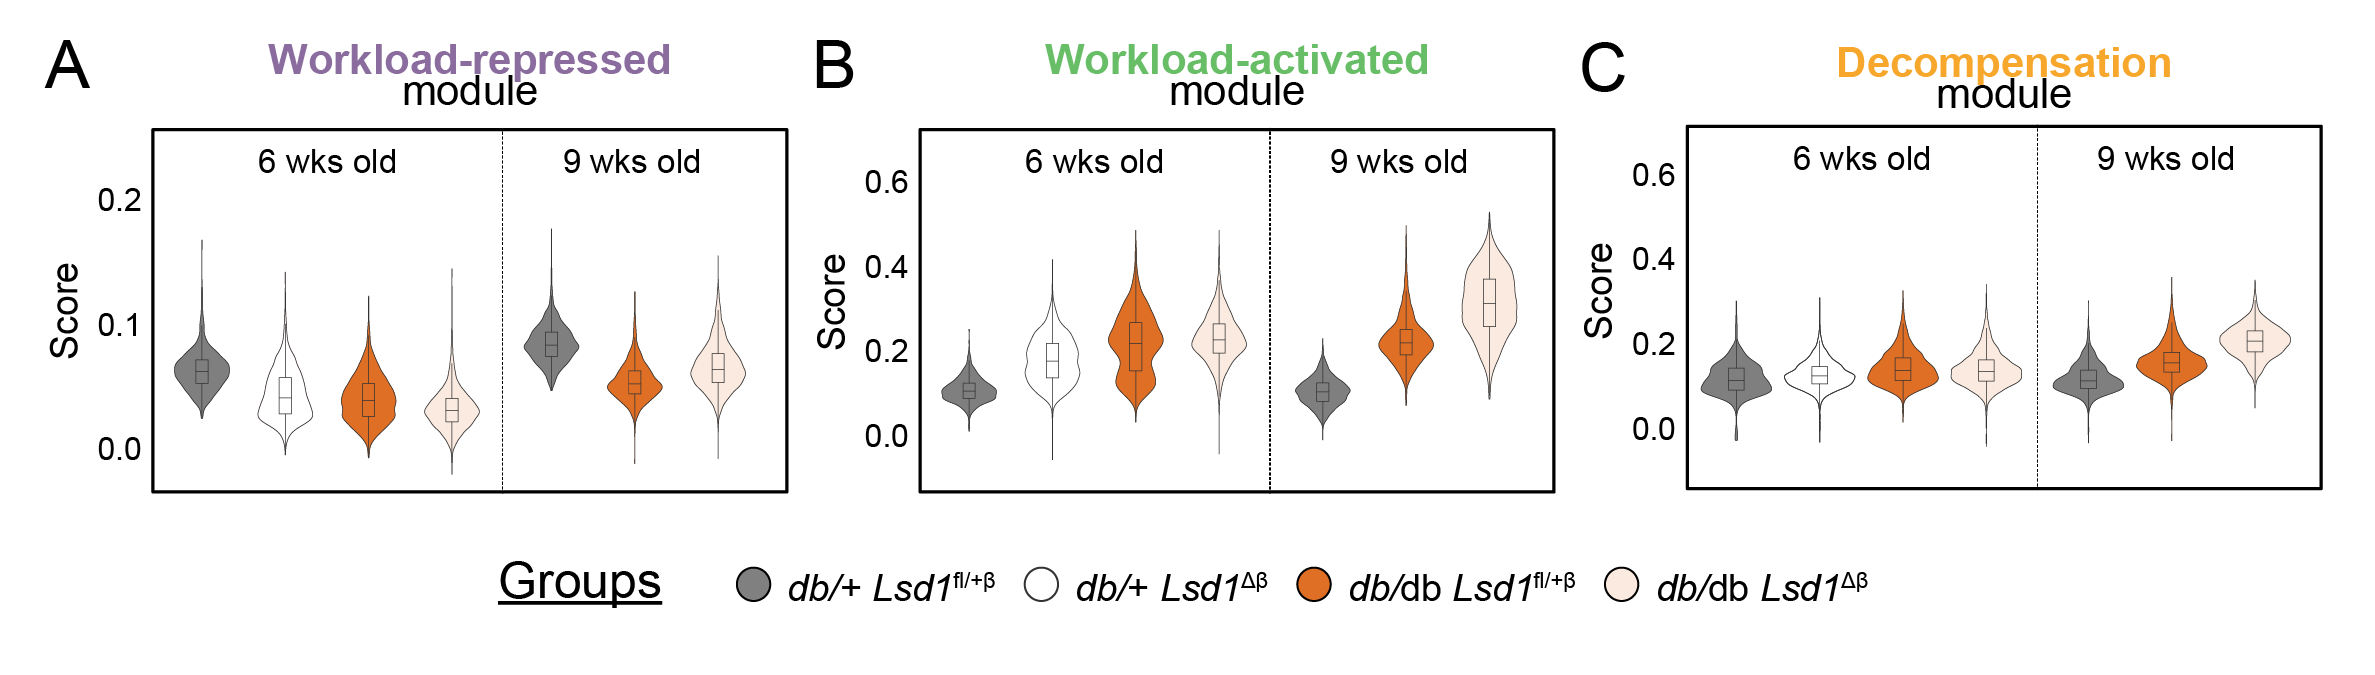
\includegraphics[width=\linewidth]{Chapter5/Fig/F3-17-01.png}
    \caption[Activity of workload-associated gene modules in the query dataset]{\textbf{Activity of workload-associated gene modules due to overworking β-cells through \textit{Lsd1} inactivation during obesity.} \textbf{(A)} Violin plots depicting the score for `Workload-repressed' module for all experimental groups across the 6-wks and 9-wks old mice in the query dataset. \textbf{(B)} Violin plots depicting the score for `Workload-activated' module for all experimental groups across the 6-wks and 9-wks old mice in the query dataset. \textbf{(C)} Violin plots depicting the score for `Decompensation' module for all experimental groups across the 6-wks and 9-wks old mice in the query dataset. For all violin plots,on the overlay box plots, the middle horizontal line represents the median, the box represents the inter-quartile range and the whiskers represent the minimum and maximum values.}
    \label{fig:chp3_valid_study_genescores}
\end{figure}

\subsubsection{\large Query mapping and Annotation transfer}

Next, we mapped our annotated β-cell subset from the integrated atlas onto the β-cells from this study \textbf{(Fig. \ref{fig:chp3_valid_study_composition})}. This allowed us to refine the compositional shifts of the identified β-cell subsets in the integrated atlas during compensatory mechanisms in response to insulin resistance during obesity. The lean animals of 6-wks-old and 9-wks-old with intact \textit{Lsd1} depicted a more representative composition of β-1 Normal and β-2 Compensating subsets (\textit{db/+ Lsd1\textsuperscript{fl/+β}}). This composition distribution is more similar to what was observed for the lean animals in the mild genetic obesity study included in the integrated analysis \textbf{(Fig. \ref{fig:3-4}D)}. Next, we could show the progressive enrichment of β-2 Compensating cells in the 6-wks-old animals - with \textit{Lsd1} deletion in the lean mice (\textit{db/+ Lsd1\textsuperscript{$\Delta$β}}), \textit{Lsd1} intact in the obese \textit{db/db} animals (\textit{db/db Lsd1\textsuperscript{fl/+β}})  and with Lsd1 deletion in \textit{db/db} animals (\textit{db/+ Lsd1\textsuperscript{$\Delta$β}})  which were primarily composed of these compensating cells. Through this mapping procedure, we were able to detect the rise and abundance of the β-3 Stress-immature subset in the older 9-wks-old \textit{db/db} animals with \textit{Lsd1} deletion (\textit{db/db Lsd1\textsuperscript{$\Delta$β}}). Interestingly, the same genotype at the 6-week time point were primarily composed of the β-2 Compensating subset. This likely suggests a shift from the compensating state in the 6-wks-old mice to a stressed-immature and decompensated state in the 9-wks-old mice, and that the β-2 Compensating and the β-3 Stress-immature cells represent different states along the axis of β-cell adaptation and decompensation.\\

\begin{figure}[t]
    \centering
    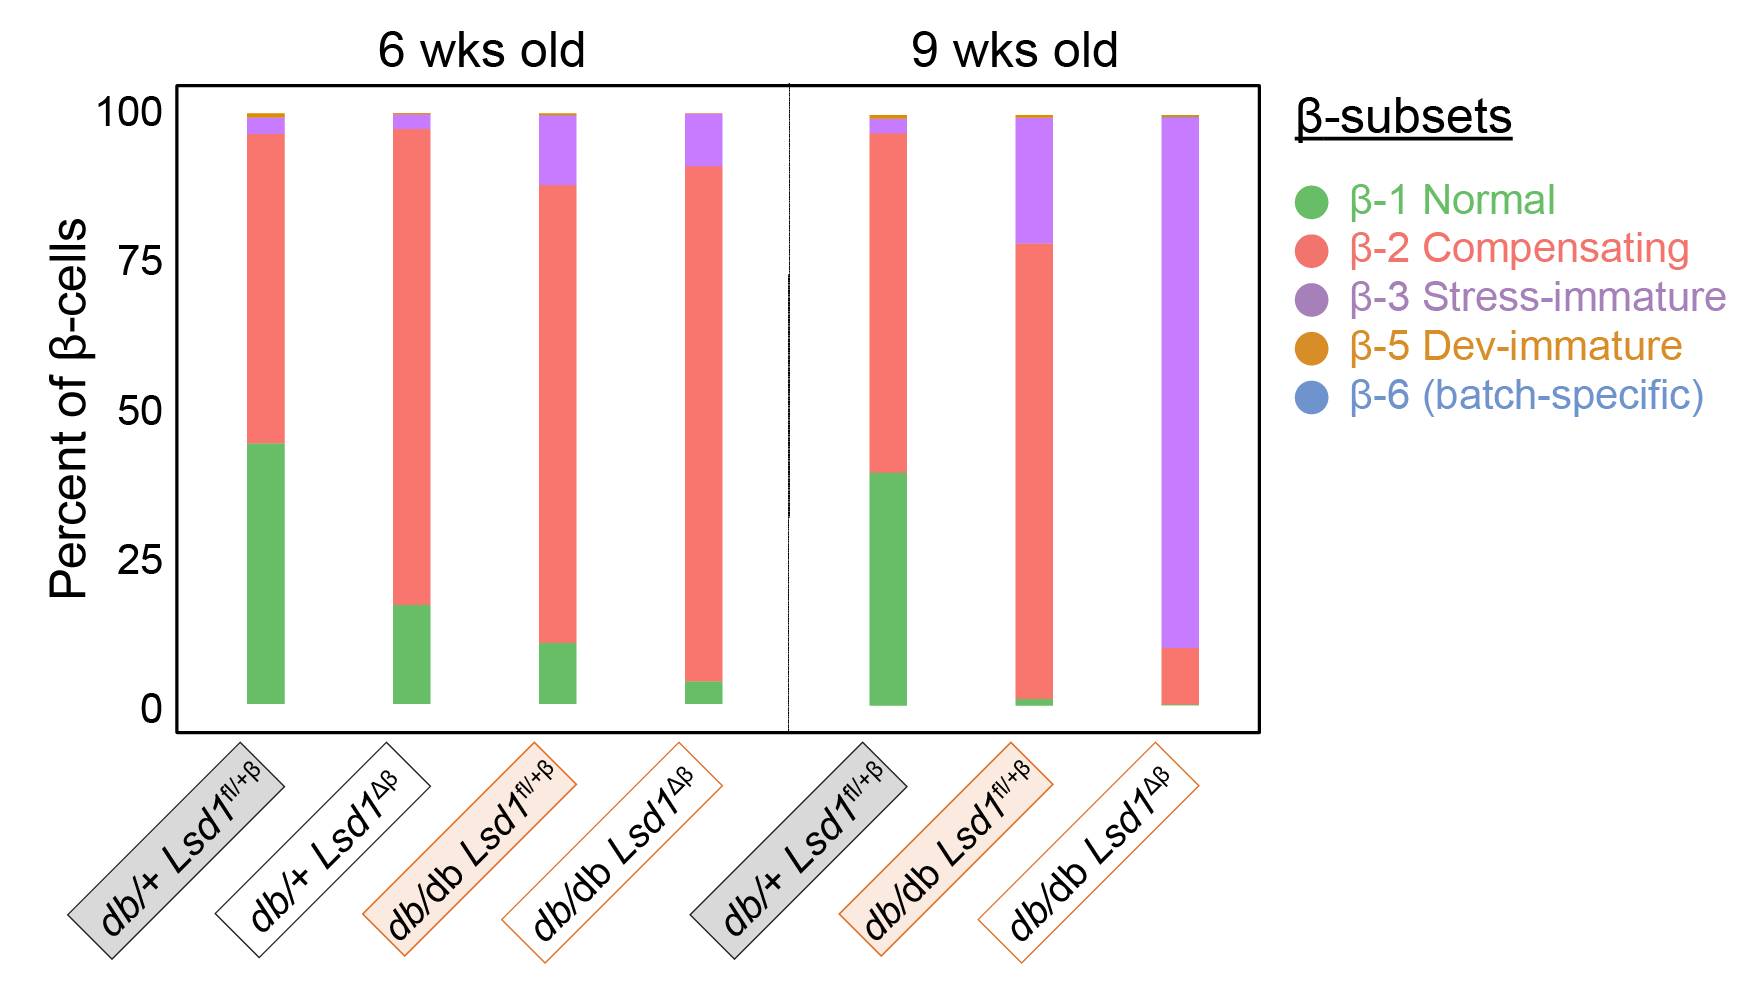
\includegraphics[width=\linewidth]{Chapter5/Fig/F3-17-03.png}
    \caption[Subtype composition shifts in the query dataset]{\textbf{Subtype composition shifts due to overworking β-cells through \textit{Lsd1} inactivation during obesity.} Bar plots depicting the composition of the experimental groups for two time-points in the query dataset, across the transferred β-cell subtype annotations from the integrated reference. The compositions were computed as percentage of cells in each subset over all cells in the group.}
    \label{fig:chp3_valid_study_composition}
\end{figure}

In summary, overworking β-cells through \textit{Lsd1} inactivation during obesity in younger animals results in progressive enrichment of the compensating subset at the expense of normal β-cells. The near total depletion of the normal β-cells in the older \textit{db/db} islets suggests that \textit{Lsd1} deletion serves to accelerate the normal disease progression with the enrichment of the compensating and the stress-immature subsets. These subtype composition shifts are correlated with the up-regulation of genes involved in increased β-cell workload and decompensation. It is likely that the subtype composition shifts observed at earlier stages simply predispose β-cells to dysfunction and failure, with the compensating phenotype being vulnerable to any subsequent stressors.


